%% Run LaTeX on this file several times to get Table of Contents,
%% cross-references, and citations.

\documentclass[11pt]{book}
\usepackage{gvv}
\usepackage{gvv-book-bkup}
%\usepackage{Wiley-AuthoringTemplate}
\usepackage[sectionbib,authoryear]{natbib}% for name-date citation comment the below line
%\usepackage[sectionbib,numbers]{natbib}% for numbered citation comment the above line

%%********************************************************************%%
%%       How many levels of section head would you like numbered?     %%
%% 0= no section numbers, 1= section, 2= subsection, 3= subsubsection %%
\setcounter{secnumdepth}{3}
%%********************************************************************%%
%%**********************************************************************%%
%%     How many levels of section head would you like to appear in the  %%
%%				Table of Contents?			%%
%% 0= chapter, 1= section, 2= subsection, 3= subsubsection titles.	%%
\setcounter{tocdepth}{2}
%%**********************************************************************%%

%\includeonly{ch01}
\makeindex

\begin{document}

\frontmatter
%%%%%%%%%%%%%%%%%%%%%%%%%%%%%%%%%%%%%%%%%%%%%%%%%%%%%%%%%%%%%%%%
%% Title Pages
%% Wiley will provide title and copyright page, but you can make
%% your own titlepages if you'd like anyway
%% Setting up title pages, type in the appropriate names here:

\booktitle{Physics }

\subtitle{Through Mathematics}

\AuAff{G. V. V. Sharma}


%% \\ will start a new line.
%% You may add \affil{} for affiliation, ie,
%\authors{Robert M. Groves\\
%\affil{Universitat de les Illes Balears}
%Floyd J. Fowler, Jr.\\
%\affil{University of New Mexico}
%}

%% Print Half Title and Title Page:
%\halftitlepage
\titlepage

%%%%%%%%%%%%%%%%%%%%%%%%%%%%%%%%%%%%%%%%%%%%%%%%%%%%%%%%%%%%%%%%
%% Copyright Page

\begin{copyrightpage}{2023}
%Title, etc
\end{copyrightpage}

% Note, you must use \ to start indented lines, ie,
% 
% \begin{copyrightpage}{2004}
% Survey Methodology / Robert M. Groves . . . [et al.].
% \       p. cm.---(Wiley series in survey methodology)
% \    ``Wiley-Interscience."
% \    Includes bibliographical references and index.
% \    ISBN 0-471-48348-6 (pbk.)
% \    1. Surveys---Methodology.  2. Social 
% \  sciences---Research---Statistical methods.  I. Groves, Robert M.  II. %
% Series.\\

% HA31.2.S873 2004
% 001.4'33---dc22                                             2004044064
% \end{copyrightpage}

%%%%%%%%%%%%%%%%%%%%%%%%%%%%%%%%%%%%%%%%%%%%%%%%%%%%%%%%%%%%%%%%
%% Only Dedication (optional) 

%\dedication{To my parents}

\tableofcontents

%\listoffigures %optional
%\listoftables  %optional

%% or Contributor Page for edited books
%% before \tableofcontents

%%%%%%%%%%%%%%%%%%%%%%%%%%%%%%%%%%%%%%%%%%%%%%%%%%%%%%%%%%%%%%%%
%  Contributors Page for Edited Book
%%%%%%%%%%%%%%%%%%%%%%%%%%%%%%%%%%%%%%%%%%%%%%%%%%%%%%%%%%%%%%%%

% If your book has chapters written by different authors,
% you'll need a Contributors page.

% Use \begin{contributors}...\end{contributors} and
% then enter each author with the \name{} command, followed
% by the affiliation information.

% \begin{contributors}
% \name{Masayki Abe,} Fujitsu Laboratories Ltd., Fujitsu Limited, Atsugi, Japan
%
% \name{L. A. Akers,} Center for Solid State Electronics Research, Arizona State University, Tempe, Arizona
%
% \name{G. H. Bernstein,} Department of Electrical and Computer Engineering, University of Notre Dame, Notre Dame, South Bend, Indiana; formerly of
% Center for Solid State Electronics Research, Arizona
% State University, Tempe, Arizona 
% \end{contributors}

%%%%%%%%%%%%%%%%%%%%%%%%%%%%%%%%%%%%%%%%%%%%%%%%%%%%%%%%%%%%%%%%
% Optional Foreword:

%\begin{foreword}
%\lipsum[1-2]
%\end{foreword}

%%%%%%%%%%%%%%%%%%%%%%%%%%%%%%%%%%%%%%%%%%%%%%%%%%%%%%%%%%%%%%%%
% Optional Preface:

%\begin{preface}
%\lipsum[1-1]
%\prefaceauthor{}
%\where{place\\
% date}
%\end{preface}

% ie,
% \begin{preface}
% This is an example preface.
% \prefaceauthor{R. K. Watts}
% \where{Durham, North Carolina\\
% September, 2004}

%%%%%%%%%%%%%%%%%%%%%%%%%%%%%%%%%%%%%%%%%%%%%%%%%%%%%%%%%%%%%%%%
% Optional Acknowledgments:

%\acknowledgments
%\lipsum[1-2]
%\authorinitials{I. R. S.}  

%%%%%%%%%%%%%%%%%%%%%%%%%%%%%%%%
%% Glossary Type of Environment:

% \begin{glossary}
% \term{<term>}{<description>}
% \end{glossary}

%%%%%%%%%%%%%%%%%%%%%%%%%%%%%%%%
%\begin{acronyms}
%\acro{ASTA}{Arrivals See Time Averages}
%\acro{BHCA}{Busy Hour Call Attempts}
%\acro{BR}{Bandwidth Reservation}
%\acro{b.u.}{bandwidth unit(s)}
%\acro{CAC}{Call / Connection Admission Control}
%\acro{CBP}{Call Blocking Probability(-ies)}
%\acro{CCS}{Centum Call Seconds}
%\acro{CDTM}{Connection Dependent Threshold Model}
%\acro{CS}{Complete Sharing}
%\acro{DiffServ}{Differentiated Services}
%\acro{EMLM}{Erlang Multirate Loss Model}
%\acro{erl}{The Erlang unit of traffic-load}
%\acro{FIFO}{First in - First out}
%\acro{GB}{Global balance}
%\acro{GoS}{Grade of Service}
%\acro{ICT}{Information and Communication Technology}
%\acro{IntServ}{Integrated Services}
%\acro{IP}{Internet Protocol}
%\acro{ITU-T}{International Telecommunication Unit -- Standardization sector}
%\acro{LB}{Local balance}
%\acro{LHS}{Left hand side}
%\acro{LIFO}{Last in - First out}
%\acro{MMPP}{Markov Modulated Poisson Process}
%\acro{MPLS}{Multiple Protocol Labeling Switching}
%\acro{MRM}{Multi-Retry Model}
%\acro{MTM}{Multi-Threshold Model}
%\acro{PASTA}{Poisson Arrivals See Time Averages}
%\acro{PDF}{Probability Distribution Function}
%\acro{pdf}{probability density function}
%\acro{PFS}{Product Form Solution}
%\acro{QoS}{Quality of Service}
%\acro{r.v.}{random variable(s)}
%\acro{RED}{random early detection}
%\acro{RHS}{Right hand side}
%\acro{RLA}{Reduced Load Approximation}
%\acro{SIRO}{service in random order}
%\acro{SRM}{Single-Retry Model}
%\acro{STM}{Single-Threshold Model}
%\acro{TCP}{Transport Control Protocol}
%\acro{TH}{Threshold(s)}
%\acro{UDP}{User Datagram Protocol}
%\end{acronyms}

\setcounter{page}{1}

\begin{introduction}
This book links high school coordinate geometry to linear algebra and matrix analysis through solved problems.

\end{introduction}

\mainmatter

\chapter{Vectors}
\section{Motion in a Plane}
\begin{enumerate}[label=\thesection.\arabic*,ref=\thesection.\theenumi]
	\item On an open ground, a motorist follows a track that turns to his left by an angle of $60\degree$ after every 500m.  Starting from a given turn, specify the displacement of the motorist at the third, sixth and eighth turn.  Compare the magnitude of the displacement with the total path length covered by the motorist in each case.
	\item Rain is falling vertically with a speed of 30 ms$^{-1}$.  A woman rides a bicycle with a speed of 10 ms$^{-1}$ in the north to south direction.  What is the direction in which she should hold her umbrella.
	\item A man can swim with a speed of 4 km/h in 
		still water.  How long does he take to cross a river 1 km wide if the river flows steadily at 3 km/h and he makes strokes normal to the river current? How far down the river does he go when he reaches the other bank?
	\item In a harbour, wind is blowing at the speed of 72 km/h and the flag on the mast of a boat anchored in the harbour flutters along the N-E direction. If the boat starts moving at a speed of 51 km/h to the north, what is the direction of the flag on the mast of the boat?
\end{enumerate}




%
\chapter{This is Chapter Two Title}

\section{This is First Level Heading}
\lipsum[1-2]

\subsection{This is Second Level Heading}
\lipsum[3]

\subsubsection{This is Third Level Heading}
\lipsum[4]

\paragraph{This is Fourth Level Heading}
\lipsum[5]

\subparagraph{This is Fifth Level Heading}
\lipsum[6] 
\backmatter
\appendix
\chapter{ Vectors}
\iffalse
\section{$2\times 1$ vectors}

%\renewcommand{\theequation}{\theenumi}
%\begin{enumerate}[label=\arabic*.,ref=\theenumi]
\begin{enumerate}[label=\thesection.\arabic*.,ref=\thesection.\theenumi]
%\begin{enumerate}[1.]
%\begin{enumerate}
%\numberwithin{equation}{enumi}
\item Let 
\begin{align}
  \vec{A} \equiv \overrightarrow{A} &= \myvec{a_1\\a_2} 
  \\
  &\equiv a_1\overrightarrow{i}+a_2\overrightarrow{j}, 
  \\
  \vec{B} &= \myvec{b_1\\b_2}, 
\end{align}
be $2 \times 1$ vectors.
Then, the determinant of the $2 \times 2$ matrix 
\begin{align}  
  \vec{M} = \myvec{\vec{A} & \vec{B}}
\end{align}
is defined as
\begin{align}
  \label{eq:det2d}
  \mydet{\vec{M}} &= \mydet{\vec{A} & \vec{B}} 
  \\
  &= \mydet{a_1 & b_1\\a_2 & b_2} = a_1b_2 - a_2 b_1
\end{align}
%
\item The value of the cross product of two vectors is given by  
  \eqref{eq:det2d}.
\item The area of the triangle with vertices $\vec{A}, \vec{B}, \vec{C}$ is given by 
	\label{prop:area2d}
\begin{align}
  \label{eq:area2d}
	\frac{1}{2}\norm{\brak{\vec{A}-\vec{B}} \times \brak{\vec{A}-\vec{C}}}
 = 
 \frac{1}{2}\norm{\vec{A} \times \vec{B}+\vec{B} \times \vec{C}+\vec{C} \times \vec{A}}
  \end{align}
  \item If 
  \label{prop:area2d-norm}
\begin{align}
  \label{eq:area2d-norm}
	\norm{\vec{A}\times\vec{B}}  &= \norm{\vec{C}\times \vec{D}}, \quad \text{then}
	\\
	\vec{A}\times\vec{B}  &= \pm\brak{\vec{C}\times \vec{D}}
  \end{align}
  where the sign depends on the orientation of the vectors.
  \item The median divides the triangle into two triangles of equal area.
	  \label{prop:two-median-area}
  \item  The transpose of $\vec{A}$ is defined as
\begin{align}
  \label{eq:transpose2d}
  \vec{A}^{\top}  = \myvec{a_1 & a_2}
\end{align}
%
\item The {\em inner product} or {\em dot product} is defined as
  \label{prop:dot2d}
\begin{align}
  \label{eq:dot2d}
  \vec{A}^{\top} \vec{B} &\equiv \vec{A} \cdot \vec{B} 
  \\
  &= \myvec{a_1 & a_2} \myvec{b_1 \\ b_2}= a_1b_1+a_2b_2 
\end{align}
%
\item {\em norm} of $\vec{A}$ is defined as
\begin{align}
  \label{eq:norm2d}
  \norm{A} &\equiv \mydet{\overrightarrow{A}}
  \\
  &= \sqrt{\vec{A}^{\top} \vec{A}}= \sqrt{a_1^2+a_2^2}
\end{align}
Thus, 
\begin{align}
  \label{eq:norm2d_const}
  \norm{\lambda \vec{A}} &\equiv \mydet{\lambda\overrightarrow{A}}
  \\
  &= \abs{\lambda} \norm{\vec{A}}
\end{align}
\item The distance betwen the points $\vec{A}$ and $\vec{B}$ is given by 
\begin{align}
  \label{eq:norm2d_dist}
\norm{\vec{A}-\vec{B}} 
\end{align}
\item Let $\vec{x}$ be equidistant from the points $\vec{A}$ and $\vec{B}$.  Then 
  \begin{align}
	  \brak{\vec{A}-\vec{B}}^{\top}{\vec{x}} 
	  =  \frac{\norm{\vec{A}}^2 - \norm{\vec{B}}^2}{2}
  \label{eq:norm2d_equidist}
  \end{align}
  \solution 
\begin{align}
	\norm{\vec{x}-\vec{A}} &=
\norm{\vec{A}-\vec{B}} 
\\
	\implies \norm{\vec{x}-\vec{A}}^2 &=
\norm{\vec{x}-\vec{B}}^2 
\end{align}
which can be expressed as 
\begin{multline}
%  \label{eq:norm2d_dist}
	\brak{\vec{x}-\vec{A}}^{\top} \brak{\vec{x}-\vec{A}}=
	\brak{\vec{x}-\vec{B}}^{\top} 
\brak{\vec{x}-\vec{B}}
\\
	\implies	\norm{\vec{x}}^2-2{\vec{x}}^{\top}\vec{A} + \norm{\vec{A}}^2
	\\= \norm{\vec{x}}^2-2{\vec{x}}^{\top}\vec{B} + \norm{\vec{B}}^2
\end{multline}
which can be simplified to obtain
  \eqref{eq:norm2d_equidist}.
\item If $\vec{x}$ lies on the  $x$-axis and is  equidistant from the points $\vec{A}$ and $\vec{B}$, 
  \begin{align}
	  \vec{x} &=
	   x\vec{e}_1
  \end{align}
  where 
  \begin{align}
	  x &=\frac{\norm{\vec{A}}^2 -\norm{\vec{B}}^2 }{2\brak{\vec{A}-\vec{B}}^{\top }\vec{e}_1
}
	  \label{eq:cbse_10_x}
  \end{align}
  \solution 
  From \eqref{eq:norm2d_equidist}.
  \begin{align}
	   x\brak{\vec{A}-\vec{B}}^{\top }\vec{e}_1
		  &=
	  \frac{\norm{\vec{A}}^2 -\norm{\vec{B}}^2 }{2}
   \end{align}
	  yielding \eqref{eq:cbse_10_x}.
  \item The angle between two vectors is given by 
    \label{prop:angle2d}
  \begin{align}
    \label{eq:angle2d}
    \theta = \cos^{-1}\frac{\vec{A}^{\top} \vec{B}}{\norm{A}\norm{B}}
  \end{align}
  \item If two vectors are orthogonal (perpendicular), 
  \begin{align}
    \label{eq:angle2d_orth}
\vec{A}^{\top} \vec{B} = 0
  \end{align}
  \item For an isoceles triangle $ABC$ ith $AB = AC$, the median $AD \perp BC$.
    \label{prop:two-isosc}
%  \begin{align}
%    \label{eq:two-isosc}
%\vec{A}^{\top} \vec{B} = 0
%  \end{align}

  \item The {\em direction vector} of the line joining two points $\vec{A},\vec{B}$ is given by 
  \begin{align}
    \label{eq:dir_vec}
    \vec{m} = \vec{A}-\vec{B}
  \end{align}
  \item The points $\vec{A}\vec{A}\vec{A}$
\item The unit vector in the direction of $\vec{m}$ is defined as
\begin{align}
    \frac{\vec{m}}{\norm{\vec{m}}}
\end{align}
\item If the direction vector of a line is expressed as 
		\label{prop:two-dir-vec}
	\begin{align}
		\label{eq:two-dir-vec}
    \vec{m} = \myvec{1\\m},
\end{align}
 the $m$ is defined to be the {\em} slope of the line. 
  \item $AB \parallel CD$ if 
	  \label{prop:two-par-dir-vec}
  \begin{align}
	  \vec{A}- \vec{B}= k\brak{\vec{C}- \vec{D}}
	  \label{eq:two-par-dir-vec}
  \end{align}
  \item The {\em normal vector} to $\vec{m}$ is defined by 
  \begin{align}
    \label{eq:normal_vec}
    \vec{m}^{\top}  \vec{n} = 0
  \end{align}
  \item  If
	  \label{prop:two-orth-para}
\begin{align}
	\vec{m}^{\top}  \vec{n}_1 &= 0
	\\
	\vec{m}^{\top}  \vec{n}_2 &= 0,
	\\
	\vec{n}_1 &\parallel \vec{n}_2
	  \label{eq:two-orth-para}
\end{align}
  \item The point $\vec{P}$ that divides the line segment $AB$ in the ratio $k:1$  is given by 

  \begin{align}
	  \vec{P}&= \frac{k\vec{B}+ \vec{A}}{k+1}
	  \label{eq:section_formula}
  \end{align}
\item  The standard basis vectors are defined as 
	\label{def:matrix-two}

  \begin{align}
  \vec{e}_1&= \myvec{1\\0}, 
  \\
  \vec{e}_2&= \myvec{0\\1}.
  \end{align}
  \item If $ABCD$ be a parallelogram,
	  \label{prop:two-pgm}
  \begin{align}
	  \label{eq:two-pgm}
 \vec{B}-\vec{A} = \vec{C} -\vec{D}
  \end{align}
  \item Diagonals of a parallelogram bisect each other.
	  \label{prop:two-pgm-diag-bisect}
\item The area of the parallelogram with vertices $\vec{A}, \vec{B}, \vec{C}$ and $\vec{D}$ is given by 
  \label{prop:pgm2d}
\begin{align}
  \label{eq:pgm2d}
	\norm{\brak{\vec{A}-\vec{B}} \times \brak{\vec{A}-\vec{D}}}
 = 
 \norm{\vec{A} \times \vec{B}+\vec{B} \times \vec{C}+\vec{C} \times \vec{A}}
  \end{align}
  \item Points $\vec{A},\vec{B}$ and $\vec{C}$ form a triangle  if 
	  \label{prop:two-tri-indep}
  \begin{align}
	  p\brak{\vec{A}- \vec{B}} +q\brak{\vec{A} -\vec{C}} &= 0
	  \\
	  \label{eq:two-tri-indep}
	  \text{or, }\brak{p+q}\vec{A}- p\vec{B} -q\vec{C} &= 0
	  \\
	  \implies p=0, q=0
  \end{align}
  are linearly independent.
  \item In $\triangle ABC$, if $\vec{D}, \vec{E}$ divide the lines $AB, AC$ in the ratio $k:1$ respectively,  then $DE \parallel BC$.
	  \label{prop:two-tri-bpt}
	  \begin{proof}
		  From 
	  \eqref{eq:section_formula}, 
  \begin{align}
	  \vec{D}&= \frac{k\vec{B}+ \vec{A}}{k+1}
	  \\
	  \vec{E}&= \frac{k\vec{C}+ \vec{A}}{k+1}
	  \\
	  \implies 
	  \vec{D}-	  \vec{E}&= \frac{k}{k+1}\brak{\vec{B}- \vec{C}}
  \end{align}
  Thus, from 
		  Appendix \ref{prop:two-dir-vec}, $DE \parallel BC$.

	  \end{proof}

  \item In $\triangle ABC$, if $DE \parallel BC$, $\vec{D}$ and $\vec{E}$ divide the lines $AB, AC$ in the same ratio.  
	  \label{prop:two-tri-bpt-conv}
	  \begin{proof}
If $DE \parallel BC$,
		  from 
 \eqref{eq:two-par-dir-vec}
  \begin{align}
	  \label{prop:two-tri-bpt-conv-1}
	  \brak{\vec{B}- \vec{C}} = k\brak{\vec{D}-	  \vec{E}}
  \end{align}
Using   
	  \eqref{eq:section_formula}, 
let 
  \begin{align}
	  \vec{D}&= \frac{k_1\vec{B}+ \vec{A}}{k_1+1}
	  \\
	  \vec{E}&= \frac{k_2\vec{C}+ \vec{A}}{k_2+1}
  \end{align}
	  Subtituting the above in 
	  \eqref{prop:two-tri-bpt-conv-1}, after some algebra, we obtain 
	
  \begin{align}
\brak{p+q}\vec{A}- p\vec{B} -q\vec{C} &= 0
  \end{align}
  where
  \begin{align}
	  p = \frac{1}{k} -  \frac{k_1}{k_1+1},
	  q = \frac{1}{k} -  \frac{k_1}{k_1+1}
  \end{align}
  %
From 	  
	  \eqref{eq:two-tri-indep},
  \begin{align}
	p = q = 0
	  \\
	  \implies k_1 = k_2  = \frac{1}{k-1}
  \end{align}

	  \end{proof}
\end{enumerate}

%
%\section{This is First Level Heading}
%\lipsum[1-2]
%
%\subsection{This is Second Level Heading}
%\lipsum[3]
%
%\subsubsection{This is Third Level Heading}
%\lipsum[4]
%
%\paragraph{This is Fourth Level Heading}
%\lipsum[5]
%
%\subparagraph{This is Fifth Level Heading}
%\lipsum[6]

%\backmatter

%\bibliography{wiley}%


%\appendix
\section{$3\times 1$ vectors}

%\renewcommand{\theequation}{\theenumi}
%\begin{enumerate}[label=\arabic*.,ref=\theenumi]
\begin{enumerate}[label=\thesection.\arabic*.,ref=\thesection.\theenumi]
%\begin{enumerate}
%\numberwithin{equation}{enumi}

\item Let 
\begin{align}
  \vec{A} &= \myvec{a_1\\a_2 \\ a_3} \equiv a_1\overrightarrow{i}+a_2\overrightarrow{j}+a_3\overrightarrow{j}, 
  \\
  \vec{B} &= \myvec{b_1\\b_2 \\ b_3}, 
\end{align}
and 
\begin{align}
  \vec{A}_{ij} &= \myvec{a_i\\a_j}, 
  \\
  \vec{B}_{ij} &= \myvec{b_i\\b_j}. 
\end{align}

\item The {\em cross product} or {\em vector product} of $\vec{A}, \vec{B}$ is defined as
\begin{align}
  \label{eq:cross3d}
	\vec{A} \times \vec{B} = \myvec{ \mydet{\vec{A}_{23} & \vec{B}_{23}} \\[10pt] \mydet{\vec{A}_{31} & \vec{B}_{31}} \\[10pt] \mydet{\vec{A}_{12}  & \vec{B}_{12}}}
\end{align}
\item Verify that
\begin{align}
  \vec{A} \times \vec{B} = -  \vec{B} \times \vec{A} 
\end{align}
\item The area of a triangle is given by 
\begin{align}
	\frac{1}{2} \norm{  \vec{A} \times \vec{B}}
\end{align}
\item (Cauchy-Schwarz Inequality)
    \begin{align}
        \label{eq:dot-mag-ineq}
	    \abs{\vec{a}^\top\vec{b}} &\le \norm{\vec{a}}\norm{\vec{b}}
    \end{align}
    \solution
	\begin{align}
        \norm{\vec{a}-\frac{\vec{a}^\top\vec{b}}{\norm{\vec{b}}^2}\vec{b}}^2 &\ge 0 \\
        \implies \norm{\vec{a}}^2 - 2\frac{\brak{\vec{a}^\top\vec{b}}^2}{\norm{\vec{b}}^2} + \frac{\brak{\vec{a}^\top\vec{b}}^2}{\norm{\vec{b}}^2} &\ge 0 \\
        \implies \norm{\vec{a}}^2 - \frac{\brak{\vec{a}^\top\vec{b}}^2}{\norm{\vec{b}}^2} &\ge 0 \\
        \implies \norm{\vec{a}}^2\norm{\vec{b}}^2 &\ge \brak{\vec{a}^\top\vec{b}}^2 \\
    \end{align}
    yielding
        \eqref{eq:dot-mag-ineq}.
\item (Triangle Inequality)
    \begin{align}
\norm{\vec{a}+\vec{b}} &\le \norm{\vec{a}}+\norm{\vec{b}}
        \label{eq:triangle-ineq}
    \end{align}
    \solution
    Using \eqref{eq:dot-mag-ineq},
    \begin{align}
        \vec{a}^\top\vec{b} &\le \norm{\vec{a}}\norm{\vec{b}} \\
\implies        \norm{\vec{a}}^2 + 2\vec{a}^\top\vec{b} + \norm{\vec{b}}^2 &\le \norm{\vec{a}}^2 + 2\norm{\vec{a}}\norm{\vec{b}} + \norm{\vec{b}}^2 \\
\implies               \norm{\vec{a}+\vec{b}}^2 &\le \brak{\norm{\vec{a}}+\norm{\vec{b}}}^2 
    \end{align}
    yielding
        \eqref{eq:triangle-ineq}.
\end{enumerate}

\chapter{Matrices}
\section{Eigenvalues and Eigenvectors}
%\renewcommand{\theequation}{\theenumi}
%\begin{enumerate}[label=\arabic*.,ref=\theenumi]
\begin{enumerate}[label=\thesection.\arabic*.,ref=\thesection.\theenumi]
%\begin{enumerate}
%\numberwithin{equation}{enumi}
\item The eigenvalue $\lambda$ and the eigenvector $\vec{x}$  for a matrix $\vec{A}$ are defined as, 
\begin{align}
  \vec{A} \vec{x} = \lambda \vec{x}
\end{align}
\item The eigenvalues are calculated by solving the
equation
\begin{align}
  \label{eq:chareq}
f\brak{\lambda} = \mydet{\lambda \vec{I}- \vec{A} } =0
\end{align}
The above equation is known as the characteristic equation.
\item According to the Cayley-Hamilton theorem,
\begin{align}
	\label{eq:cayley}
  f(\lambda) = 0 \implies f\brak{\vec{A}} = 0
\end{align}
\item The trace of a square  matrix is defined to be the sum of the diagonal elements.
\begin{align}
	\label{eq:trace}
	\text{tr}\brak{\vec{A}}=\sum_{i=1}^{N}a_{ii}.
\end{align}
	where $a_{ii}$ is the $i$th diagonal element of the matrix $\vec{A}$. 	
\item The trace of a matrix is equal to the sum of the eigenvalues
\begin{align}
	\label{eq:trace_eig}
	\text{tr}\brak{\vec{A}}=\sum_{i=1}^{N}\lambda_i
\end{align}


\end{enumerate}
\section{Determinants}
%\renewcommand{\theequation}{\theenumi}
%\begin{enumerate}[label=\arabic*.,ref=\theenumi]
\begin{enumerate}[label=\thesection.\arabic*.,ref=\thesection.\theenumi]
%\begin{enumerate}
%\numberwithin{equation}{enumi}

\item Let 
\begin{align}
	\vec{A} = \myvec{a_1 & b_1 & c_1  \\ a_2 & b_2 & c_2  \\ a_3 & b_3 & c_3}.
\end{align}
be a $3 \times 3$ matrix. 
Then, 
\begin{multline}
	\mydet{\vec{A}} = a_1 \myvec{ b_2 & c_2 \\  b_3 & c_3} - a_2\myvec{ b_1 & c_1 \\  b_3 & c_3 }  \\ + a_3\myvec{a_1 & b_1 \\ a_2 & b_2 }.
\end{multline}
\item Let $\lambda_1,\lambda_2, \dots, \lambda_n$ be the eigenvalues of a matrix $\vec{A}$.  Then,   the product of the eigenvalues is equal to the determinant of $\vec{A}$.
\begin{align}
	\mydet{\vec{A}} = \prod_{i=1}^{n}\lambda_i
\end{align}
%
\item 
\begin{align}
	\mydet{\vec{A}\vec{B}} = \mydet{\vec{A}}\mydet{\vec{B}}
\end{align}
\item If $\vec{A}$ be an $n \times n$ matrix, 
\begin{align}
	\label{eq:det_kord}
	\mydet{k\vec{A}} = k^n\mydet{\vec{A}}
\end{align}

\end{enumerate}
\section{Rank of a Matrix}
%\renewcommand{\theequation}{\theenumi}
%\begin{enumerate}[label=\arabic*.,ref=\theenumi]
\begin{enumerate}[label=\thesection.\arabic*.,ref=\thesection.\theenumi]
%\begin{enumerate}
%\numberwithin{equation}{enumi}
\item The rank of a matrix is defined as the number of linearly independent rows.  This is also known as the row rank.
\item Row rank = Column rank.
\item The rank of a matrix is obtained as the number of nonzero rows obtained after row reduction.
\item An $n \times n$ matrix is invertible if and only if its rank is $n$.

\item Points $\vec{A}, \vec{B}, \vec{C}$ are on a line if 
\begin{align}
%  \label{eq:line_rank}
  \text{rank}\myvec{\vec{A} \\ \vec{B} \\ \vec{C} }  = 1
\end{align}
\item Points $\vec{A}, \vec{B}, \vec{C}, \vec{D}$ form a paralelogram if 
\begin{align}
%  \label{eq:parallelgm_rank}
  \text{rank}\myvec{\vec{A} \\ \vec{B} \\ \vec{C} \\ \vec{D}  }  = 1, 
  \text{rank}\myvec{\vec{A} \\ \vec{B} \\ \vec{C} }  = 2
\end{align}
\end{enumerate}
\section{Inverse of a Matrix}
%\renewcommand{\theequation}{\theenumi}
%\begin{enumerate}[label=\arabic*.,ref=\theenumi]
\begin{enumerate}[label=\thesection.\arabic*.,ref=\thesection.\theenumi]
%\begin{enumerate}
%\numberwithin{equation}{enumi}
\item For a $2 \times 2$ matrix 
\begin{align}
	\vec{A} = \myvec{a_1 & b_1  \\ a_2 & b_2 },
\end{align}
the inverse is given by 
\begin{align}
	\vec{A}^{-1} = \frac{1}{\mydet{\vec{A}}}\myvec{b_2 & -b_1  \\ -a_2 & a_1 },
\end{align}
\item For higher order matrices, the inverse should be calculated using row operations.
\end{enumerate}
\section{Orthogonality}
%\renewcommand{\theequation}{\theenumi}
%\begin{enumerate}[label=\arabic*.,ref=\theenumi]
\begin{enumerate}[label=\thesection.\arabic*.,ref=\thesection.\theenumi]
%\begin{enumerate}
%\numberwithin{equation}{enumi}
\item The rotation matrix is defined as 
\begin{align}
	\vec{R}_{\theta} = \myvec{\cos \theta & -\sin \theta  \\ \sin \theta  & \cos \theta  }, \quad \theta \in \sbrak{0, 2\pi}
\end{align}
\item The rotation matrix is {\em orthogonal}
\begin{align}
	\vec{R}_{\theta}^{\top}\vec{R}_{\theta} = \vec{R}_{\theta}\vec{R}_{\theta}^{\top} = \vec{I}
\end{align}
\item If the angle of rotation is $\frac{\pi}{2}$,
	\label{prop:mat/rot/pi/2}
\begin{align}
	\vec{m}^{\top}\vec{n} = 0 \implies \vec{n} = \vec{R}_{\frac{\pi}{2}}\vec{m}
\end{align}
\item 
\begin{align}
	\label{eq:mat-nh}
	\vec{n}^{\top}\vec{h} = 1 \implies \vec{n} = \frac{\vec{e}_1}{\vec{e}_1^{\top}\vec{h}}+\mu\vec{R}_{\frac{\pi}{2}}\vec{h}, \quad \mu \in \mathbb{R}.
\end{align}


\item
	The {\em affine} transformation is given by 
    \begin{align}
	    \vec{x} &= \vec{P}\vec{y}+\vec{c} \quad \text{(Affine Transformation)}
\label{eq:conic_affine}
    \end{align}
	where $\vec{P}$ is invertible.

\item
	The eigenvalue decomposition of a symmetric matrix $\vec{V}$ is given by 
	%\cite{banchoff}
    \begin{align}
      \label{eq:conic_parmas_eig_def}
      \vec{P}^{\top}\vec{V}\vec{P} &= \vec{D}. \quad \text{(Eigenvalue Decomposition)}
      \\
      \vec{D} &= \myvec{\lambda_1 & 0\\ 0 & \lambda_2}, 
      \\
      \vec{P} &= \myvec{\vec{p}_1 & \vec{p}_2}, \quad \vec{P}^{\top}=\vec{P}^{-1},
      \label{eq:eigevecP}
    \end{align}


\end{enumerate}

\section{Singular Value Decomposition}
\renewcommand{\theequation}{\theenumi}
\begin{enumerate}[label=\thesection.\arabic*.,ref=\thesection.\theenumi]
\numberwithin{equation}{enumi}

\item 
\iffalse
	We revisit \eqref{eq:pseudo_mat_eq}
%
\begin{align}
\myvec{
1 & 2
\\
-1 & 1
\\
1 & 2
}
\vec{x} =
\myvec{1 \\ -3 \\ -2}
\end{align}
\fi
\item Consider the rectangular equation
\begin{align}
	\vec{M}^{\top}\vec{x}=\vec{b}
\label{eq:pseudo_mat_eq}
\end{align}

\item Find $\vec{M}^T\vec{M}$ and $\vec{M}\vec{M}^T$.
\item Obtain the eigen decomposition 
\begin{align}
\vec{M}^T\vec{M} = \vec{P}_1\vec{D}_1\vec{P}_1^T
\end{align}
and 
\begin{align}
\vec{M}\vec{M}^T = \vec{P}_2\vec{D}_2\vec{P}_2^T
\end{align}
\item Perform the $QR$ decompositions
\begin{align}
\vec{P}_1 = \vec{U}\vec{R}_1,\,
\vec{P}_2 = \vec{V}\vec{R}_2
\end{align}
\item The singular value decomposition is the given by
\begin{align}
\vec{M} = \vec{U} \Sigma \vec{V}^T,
\end{align}
where $\Sigma$ has the same shape as $\vec{M}$ and
\begin{align}
\Sigma = \myvec{\vec{D}_1 & \vec{0} \\ \vec{0} & \vec{0}}
\end{align}
\item \eqref{eq:pseudo_mat_eq} can then be expressed as
\begin{align}
\vec{U} \Sigma \vec{V}^T \vec{x} &= \vec{b}
\\
\implies \vec{x} & = \vec{V}\Sigma^{-1} \vec{U}^T \vec{b}
\end{align}
%
where $\vec{\Sigma}^{-1}$ is obtained by inverting  only the non-zero elements of $\vec{\Sigma}$.
\iffalse
\item The relevant codes are available at
\begin{lstlisting}
codes/line/skew_builtin.py
codes/line/skew_svd.py
\end{lstlisting}
\fi
\end{enumerate}


\chapter{Triangle Constructions}
\begin{enumerate}[label=\thesection.\arabic*,ref=\thesection.\theenumi]
\numberwithin{equation}{enumi}
\numberwithin{figure}{enumi}
\numberwithin{table}{enumi}
\item 
	Construct a triangle $ABC$ in which $a, \angle{B}$ and $c + b  = K$ are given.
\label{cons/tri/1}
	\\
	\solution 
\iffalse
\documentclass[10pt,a4paper]{report}
\usepackage[latin1]{inputenc}
\usepackage{amsmath}
\usepackage{amsfonts}
\usepackage{amssymb}
\usepackage{graphicx}
\usepackage{hyperref}
\usepackage{multicol}
\usepackage[margin=0.1 in]{geometry}
\usepackage{tikz}
\usepackage{romannum}
\usepackage{listings}
\usetikzlibrary{arrows,shapes.gates.logic.US,shapes.gates.logic.IEC,calc}
\usepackage{titlesec}
\titlespacing{\subsection}{1pt}{\parskip}{3pt}
\titlespacing{\subsubsection}{0pt}{\parskip}{-\parskip}
\titlespacing{\paragraph}{0pt}{\parskip}{\parskip}
\newcommand{\myvec}[1]{\ensuremath{\begin{pmatrix}#1\end{pmatrix}}}
\let\vec\mathbf

\begin{document}

\centering {
\includegraphics[scale=0.07]{IITH.png}} \vspace{3mm}\\ \raggedleft Name:T.Manasa Reddy\vspace{2mm}\\ \raggedleft Roll No.: FWC22048\vspace{2mm}\\ \raggedright Sep 2022 \hspace{12cm} \raggedleft manasatanuboddi@gmail.com \vspace{10mm}
\\ \centering \Large \textbf{MATRIX ASSIGNMENT} \normalsize \vspace{15mm}

\begin{multicols}{2}
\section{Problem:}  
\fi
	\iffalse
	See Fig. 
		\ref{eq:cons/tri/9/11/2/1}.
	\begin{figure}[!h]
		\centering
 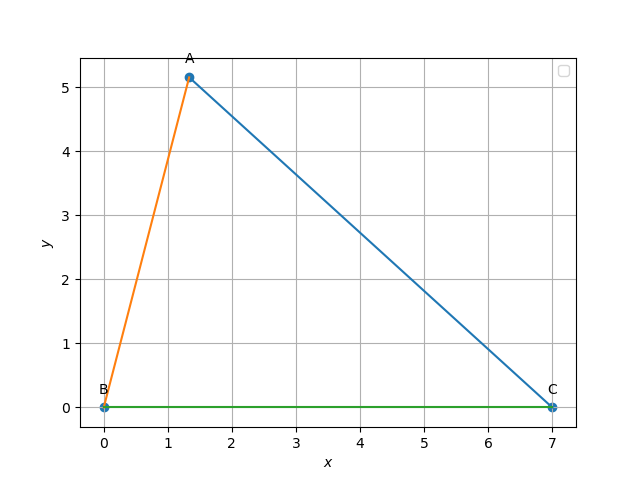
\includegraphics[width=\columnwidth]{chapters/9/11/2/1/figs/Figure_1.png}
		\caption{}
		\label{eq:cons/tri/9/11/2/1}
  	\end{figure}
	
	\vspace{3mm}
\section{Solution}
The input parameters for this construction are
\begin{center}
\begin{tabular}{|c|c|c|}
	\hline
	\textbf{Symbol}&\textbf{Value}&\textbf{Description}\\
	\hline
	BC & a & where a is 7cm\\
	\hline
	AB & b & AB distance is b \\
	\hline 
	AC & c & AC distance is c \\
	\hline
	$\angle{BC}$ & $75^0$ &  $\triangle$ABC \\
	\hline
	$\vec{C}$ & $\myvec{a\\0}$ & BC length is equal to a\\
	\hline
	$\vec{A}$ & $\myvec{ \cos\theta \\ \sin\theta}$ & using the cosine formula in $\triangle$ABC\\
	\hline
\end{tabular}
\end{center}
\raggedright {termux commands :}
\begin{center}
\fbox{\parbox{8.5cm}{bash line.sh.........using shell command}}
\end{center}
\raggedright\textbf{Caluclating Other Coordinate: } \\
\raggedright Let the coordinates of A are $X_{2}$,$Y_{2}$ respectively. \\
  \raggedright Let \textbf{A} =
  $\begin{pmatrix} 
 \cos \theta\\
  \sin\theta \\
\end{pmatrix}$ \\
\raggedright 
\fi
	Using the cosine formula in  $\triangle ABC$,
\begin{align}
	{b}^2&= {a}^2 + {c}^2 - 2ac\cos{B}
\\
\implies	(b+c)(b-c) &= {a}^2- 2  a  c\cos{B}
\\
	\text{or, }K(b-c) &= {a}^2- 2  a  c\cos{B}
		\label{eq:cons/tri/9/11/2/1/k}
\end{align}
%
where
\begin{align}
K = b+c 
		\label{eq:cons/tri/9/11/2/1/k/def}
\end{align}
From 
		\eqref{eq:cons/tri/9/11/2/1/k}
		and
		\eqref{eq:cons/tri/9/11/2/1/k/def},
\begin{align}
	\myvec{
		1 & 1
		\\
		1 & -1 
	}
	\myvec{
	b
	\\
	c
	}
	&=
	\myvec{
		\frac{{a}^2- 2  a  c\cos{B}}{K}
		\\
K}
\\
\implies
	\myvec{
	b
	\\
	c
	}
	&=
	\frac{1}{2}\myvec{
		1 & 1
		\\
		1 & -1 
	}
	\myvec{
		\frac{{a}^2- 2  a  c\cos{B}}{K}
	\\
K}
		\label{eq:cons/tri/9/11/2/1/k/mateq}
\\
\because
\myvec{
		1 & 1
		\\
		1 & -1 }
	\myvec{
		1 & 1
		\\
		1 & -1 }
	&	= 	{2}\vec{I}
\end{align}
From 
		\eqref{eq:cons/tri/9/11/2/1/k/mateq}
\begin{align}
	c
	&=
	\frac{1}{2}\vec{e}_2^{\top}\myvec{
		1 & 1
		\\
		1 & -1 
	}
	\myvec{
		\frac{{a}^2}{K}
	\\
	K}- \frac{2  a  c\cos{B}}{K}
\\
\implies
	c &=
	\frac{1}{2\brak{1+ \frac{2  a  \cos{B}}{K}}}\vec{e}_2^{\top}\myvec{
		1 & 1
		\\
		1 & -1 
	}
	\myvec{
		\frac{{a}^2}{K}
	\\
K}
\end{align}
The coordinates of $\triangle ABC$ can then be expressed as
\begin{align}
	\vec{A}=c\myvec{\cos B \\ \sin B},
	\vec{B} = \vec{0},
	\vec{C} =\myvec{a \\ 0}.
\end{align}
\iffalse
   reduced row echelon form of $\begin{pmatrix}13 & -13 + \frac{\sqrt{2} (-7 + 7 \sqrt{3})}{2} & 49\\1 & 1 & 13\end{pmatrix}$
        \vspace{3mm}
        \\Divide row1 by 13: R1 = $\frac{R1}{13}$
        \vspace{7mm}
 $        \begin{pmatrix} 1 & -\frac{ -7\sqrt{6}  + 7 \sqrt{2} + 26 )}{26} & \frac{49}{13}\\ 1& 1 & 13\end{pmatrix}$ \vspace{5mm}
        \\ Subtract row 1 from row 2: R2 = R2 - R1 \vspace{3mm}
        \\ $\begin{pmatrix}1 & -\frac{ -7\sqrt{6}  + 7 \sqrt{2} + 26 )}{26} & \frac{49}{13}\\ 0 & -\frac{ -7\sqrt{6}  + 7 \sqrt{2} + 52 )}{26} & \frac{120}{13}\end{pmatrix}$ \vspace{6mm}
         Multiply row 2 by $\frac{26}{- 7 \sqrt{6} + 7 \sqrt{2} + 52}$:\vspace{3mm}
         R2=$\frac{26}{- 7 \sqrt{6} + 7 \sqrt{2} + 52}$  
         \vspace{6mm}
    \\ Add row 2 multiplied by $\frac{- 7 \sqrt{6} + 7 \sqrt{2} + 26}{26}$ \vspace{5mm}
     \\  $\begin{pmatrix}1 & 0 &-\frac{ 91\sqrt{6}  + 91\sqrt{2} + 436)}{-7\sqrt{6}  + 7 \sqrt{2} + 52 )}\\ 0 & 1 &\frac{240}{ -7\sqrt{6} + 7 \sqrt{2} + 52} \end{pmatrix} $ \vspace{5mm}
     \\ $\begin{pmatrix}
     b \\
     c \\
     \end{pmatrix}$%
     = $\begin{pmatrix}
     -\frac{ 91\sqrt{6}  + 91\sqrt{2} + 436)}{-7\sqrt{6}  + 7 \sqrt{2} + 52 )} \\
     \frac{240}{ -7\sqrt{6} + 7 \sqrt{2} + 52}
     \end{pmatrix}$%
     \vspace{5mm}
    \\ \raggedright \textbf{A} = c$\begin{pmatrix}
                 \cos 75 \\ 
                 \sin 75 \\
              \end{pmatrix}$%
              =$\begin{pmatrix}
                 1.33 \\
                 5.15 \\
                 \end{pmatrix}$%
                 \vspace{5mm}
              \\ \raggedright  \textbf{B} = $\begin{pmatrix}
                 0\\
                 0\\
              \end{pmatrix}$% 
              \vspace{5mm}
             \\ \raggedright  \textbf{C} = $\begin{pmatrix}
                  7\\
                  0\\
              \end{pmatrix}$%
              \vspace{5mm}
\\
Below python code realizes the above construction : 
\fbox{\parbox{8.5cm}{\url{https://github.com/manasareddy442002/fwc-moudle1/blob/matrix-lines/matrix.py}}}

 \section{Construction}
 	\begin{center}
  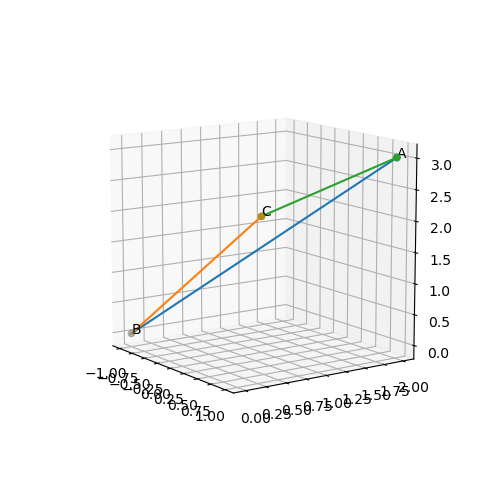
\includegraphics[scale=0.5]{Figure_1.png}
  	\end{center}
\vspace{3cm}
\end{multicols}

\end{document}
\fi

%
\iffalse
\item 
\label{cons/tri/2}
\iffalse
\documentclass[10pt,a4paper]{report}
\usepackage[latin1]{inputenc}
\usepackage{amsmath}
\usepackage{amsfonts}
\usepackage{amssymb}
\usepackage{graphicx}
\usepackage{hyperref}
\usepackage{multicol}
\usepackage[margin=0.5in]{geometry}
\usepackage{tikz}
\usepackage{romannum}
\usepackage{listings}
\usetikzlibrary{arrows,shapes.gates.logic.US,shapes.gates.logic.IEC,calc}
\usepackage{titlesec}
\titlespacing{\subsection}{1pt}{\parskip}{3pt}
\titlespacing{\subsubsection}{0pt}{\parskip}{-\parskip}
\titlespacing{\paragraph}{0pt}{\parskip}{\parskip}
\newcommand{\myvec}[1]{\ensuremath{\begin{pmatrix}#1\end{pmatrix}}}
\let\vec\mathbf

\begin{document}

\centering {
\includegraphics[scale=0.07]{IIT.png}} \vspace{3mm}\\ \raggedleft Name:Somisetty.Kedareswari\vspace{2mm}\\ \raggedleft Roll No.: FWC22049\vspace{2mm}\\ \raggedright Sep 2022 \hspace{12cm} \raggedleft mail2kedari@gmail.com \vspace{10mm}
\\ \centering \Large \textbf{MATRIX ASSIGNMENT} \normalsize \vspace{15mm}
\begin{multicols}{2}
\section{Problem:}  
\fi
	Construct a triangle $ABC$ in which $BC=8cm, \angle{B}=45\degree$ and $AB - AC = 3.5 cm$.
	\solution 
	See Fig. 
		\ref{fig:9/11/2/2}.
	\begin{figure}[!h]
		\centering
 \includegraphics[width=\columnwidth]{chapters/9/11/2/2/figs/Fig.png}
		\caption{}
		\label{fig:9/11/2/2}
  	\end{figure}
	Using the cosine formula in  $\triangle ABC$,
\begin{align}
	{b}^2&= {a}^2 + {c}^2 - 2ac\cos{B}
\\
\implies	(b+c)(b-c) &= {a}^2- 2  a  c\cos{B}
\\
	\text{or, }K(b+c) &= {a}^2- 2  a  c\cos{B}
		\label{fig:9/11/2/2/k}
\end{align}
%
where
\begin{align}
-K = b-c 
		\label{fig:9/11/2/2/k/def}
\end{align}
From 
		\eqref{fig:9/11/2/2/k}
		and
		\eqref{fig:9/11/2/2/k/def},
\begin{align}
	\myvec{
		1 & 1
		\\
		1 & -1 
	}
	\myvec{
	b
	\\
	c
	}
	&=
	\myvec{
		\frac{{a}^2- 2  a  c\cos{B}}{K}
		\\
-K}
\\
\implies
	\myvec{
	b
	\\
	c
	}
	&=
	\frac{1}{2}\myvec{
		1 & 1
		\\
		1 & -1 
	}
	\myvec{
		\frac{{a}^2- 2  a  c\cos{B}}{K}
	\\
-K}
		\label{fig:9/11/2/2/k/mateq}
\\
\because
\myvec{
		1 & 1
		\\
		1 & -1 }
	\myvec{
		1 & 1
		\\
		1 & -1 }
	&	= 	{2}\vec{I}
\end{align}
From 
		\eqref{fig:9/11/2/2/k/mateq}
\begin{align}
	c
	&=
	\frac{1}{2}\vec{e}_2^{\top}\myvec{
		1 & 1
		\\
		1 & -1 
	}
	\myvec{
		\frac{{a}^2}{K}
	\\
	-K}- \frac{2  a  c\cos{B}}{K}
\\
\implies
	c &=
	\frac{1}{2\brak{1+ \frac{2  a  \cos{B}}{K}}}\vec{e}_2^{\top}\myvec{
		1 & 1
		\\
		1 & -1 
	}
	\myvec{
		\frac{{a}^2}{K}
	\\
-K}
\end{align}
The coordinates of $\triangle ABC$ can then be expressed as
\begin{align}
	\vec{A}=c\myvec{\cos B \\ \sin B},
	\vec{B} = \vec{0},
	\vec{C} =\myvec{a \\ 0}.
\end{align}

	\iffalse
\section{Solution}
The input parameters for this construction are
\begin{center}
\begin{tabular}{|c|c|c|}
  \hline
  \textbf{Symbol}&\textbf{Value}&\textbf{Description}\\
  \hline
  BC & a & where a is 8cm\\
  \hline
  $\angle{BC}$ & $45^0$ &  $\Delta$ABC \\
  \hline
  k & 3.5 & constant value\\
  \hline
\end{tabular}
\end{center}
\raggedright\textbf{Caluclating Other Coordinate: } \\
\raggedright The coordinates of B and C are $X_{2}$,$Y_{2}$ respectively. \\
  \raggedright Let \textbf{A} = c$\times$
  $\begin{pmatrix} 
 \cos \theta\\
  \sin\theta \\
\end{pmatrix}$ \\
\raggedright Using the Cosine formula in  $\Delta$ABC, \\ \vspace{3mm}
\begin{equation}
{b}^2\hspace{1.5cm}= {a}^2 + {c}^2 - 2accos\vec{B}
\end{equation}
\begin{equation}
(b+c)(b-c) = {a}^2- 2accos\vec{B}
\end{equation}
Given
\begin{equation}
        c-b=k
\end{equation}\\
Upon Simplifaction we get:- \\
\begin{equation}
  (b+c)(-k) = {a}^2- 2accos\vec{B} 
\end{equation}
\begin{equation}
-kc-kb+2accos\vec{B}= {a}^2
\end{equation}
\begin{equation}
-kb-c(-k+2acos\vec{B})= {a}^2
\end{equation}
     From the above, we obtain the matrix equation:- \\ \vspace{3mm}
        $\begin{pmatrix}
            -k & k+2acos\vec{B}  \\
            -1 & 1  \\
        \end{pmatrix}$% 
        $\begin{pmatrix}
            c \\
            b \\
        \end{pmatrix}$% 
           =
           $\begin{pmatrix}
            k\\
            a^2\\
        \end{pmatrix}$%   
        \vspace{5mm}           
   \\  
    $\begin{pmatrix}
            -3.5 & 3.5+2(8)cos45^0 \\
            -1 & 1  \\
        \end{pmatrix}$% 
        $\begin{pmatrix}
            c \\
            b \\
        \end{pmatrix}$% 
           =
           $\begin{pmatrix}
            3.5\\
            64\\
        \end{pmatrix}$%   
        \vspace{5mm}           
   \\  
   Augmented Matrix $\implies$
   $\begin{pmatrix}
         -3.5 & 3.5+2(8)cos45^0 & 3.5\\
            -1 & 1  & 64\\
          \\
    \end{pmatrix}$%
    \\
    Reducing to echelon form:-
   \\
    $\begin{pmatrix}
    \myvec{1&-1&\frac{7}{2} \\ -\frac{7}{2}&\frac{78154172560113}{10000000000000}&64}
    \xleftarrow[]{-R_1 \leftarrow R_1}
    \end{pmatrix}$%
  \\
  \vspace{5mm}
   $\begin{pmatrix}
    \myvec{1&-1&\frac{7}{2} \\ 0&1&\frac{517500000000000}{43154172560113}}
    \xleftarrow[]{\frac{10000000000000R2}{43154172560113} \leftarrow R_2}
    \end{pmatrix}$%
  \\
  \vspace{5mm}
  $\begin{pmatrix}
    \myvec{1&0&\frac{732920792079209}{86308345120226} \\ 0&1&\frac{517500000000000}{43154172560113}}
    \xleftarrow[]{R1+R2 \leftarrow R_2}
    \end{pmatrix}$%
  \\
  \vspace{5mm}
  Reduced Echelon Form: 
  $\begin{pmatrix}
    \myvec{1&0&8.491887905604763 \\ 0&1&11.991887905604763}
    \end{pmatrix}$% 
    \\
    \vspace{5mm}
      $\begin{pmatrix}
            c\\
            b\\
        \end{pmatrix}$% 
            =
            $\begin{pmatrix}
            11.99\\
            8.49\\
        \end{pmatrix}$% 
        \vspace{3mm}
   \\  The vertices of $\Delta$ ABC are \\ \vspace{3mm}
     \raggedright \textbf{A} = 11.99$\begin{pmatrix}
                 cos 45 \\ 
                 sin 45 \\
              \end{pmatrix}$%
              =$\begin{pmatrix}
                 8.4 \\
                 8.4 \\
                 \end{pmatrix}$%
                 \vspace{5mm}
              \\ \raggedright  \textbf{B} = $\begin{pmatrix}
                 0\\
                 0\\
              \end{pmatrix}$% 
              \vspace{5mm}
             \\ \raggedright  \textbf{C} = $\begin{pmatrix}
                  8\\
                  0\\
              \end{pmatrix}$%
              \\
Below python code realizes the above construction : 
\fbox{\parbox{8.5cm}{\url{https://github.com/kedareswari200/fwc-moudle1/blob/Matri_lines/triangle.py}}}
 \\
 \section{Construction}
   \begin{center}
  \includegraphics[scale=0.5]{Fig.png}
    \end{center}
\vspace{3cm}
\end{multicols}

\end{document}
\fi

%
\item 
\label{cons/tri/3}
\iffalse
\documentclass[10pt,a4paper]{article}
\usepackage{amsmath}
\usepackage{amsfonts}
\usepackage{amssymb}
\usepackage{graphicx}
\usepackage{multicol}
\usepackage{tabularx}
\usepackage{tikz}
\usetikzlibrary{arrows,shapes,automata,petri,positioning,calc}
\usepackage{hyperref}
\usepackage{tikz}
\usepackage{gensymb}
\usepackage{polynom}
\usetikzlibrary{matrix,calc}
\makeatletter
\newcommand\xleftrightarrow[2][]{%
  \ext@arrow 9999{\longleftrightarrowfill@}{#1}{#2}}
\newcommand\longleftrightarrowfill@{%
  \arrowfill@\leftarrow\relbar\rightarrow}
\makeatother
\usepackage[margin=0.5in]{geometry}
\newcommand{\myvec}[1]{\ensuremath{\begin{pmatrix}#1\end{pmatrix}}}
\let\vec\mathbf
\newenvironment{Figure}
  {\par\medskip\noindent\minipage{\linewidth}}
  {\endminipage\par\medskip}
\begin{document}
%--------------------logo figure-------------------------%
\begin{figure*}[!tbp]
 \centering
  \begin{minipage}[b]{0.4\textwidth}
  
\includegraphics[scale=.25]{iitlogo.png} 
  \end{minipage}
\end{figure*}
%--------------------name & rollno-----------------------
\raggedright \textbf{Name}:\hspace{1mm} Ganga Gopinath\hspace{3cm} \Large \textbf{Matrix Assignment}\hspace{2.5cm} % 
\normalsize \textbf{Roll No.} :\hspace{1mm} FWC22050\vspace{1cm}
\begin{multicols}{2}
\section{Problem statement:}
\fi
	Construct a triangle $PQR$ in which $QR=6cm, \angle{Q}=60\degree$ and $PR - PQ = 2cm$.
	\begin{figure}[!h]
		\centering
 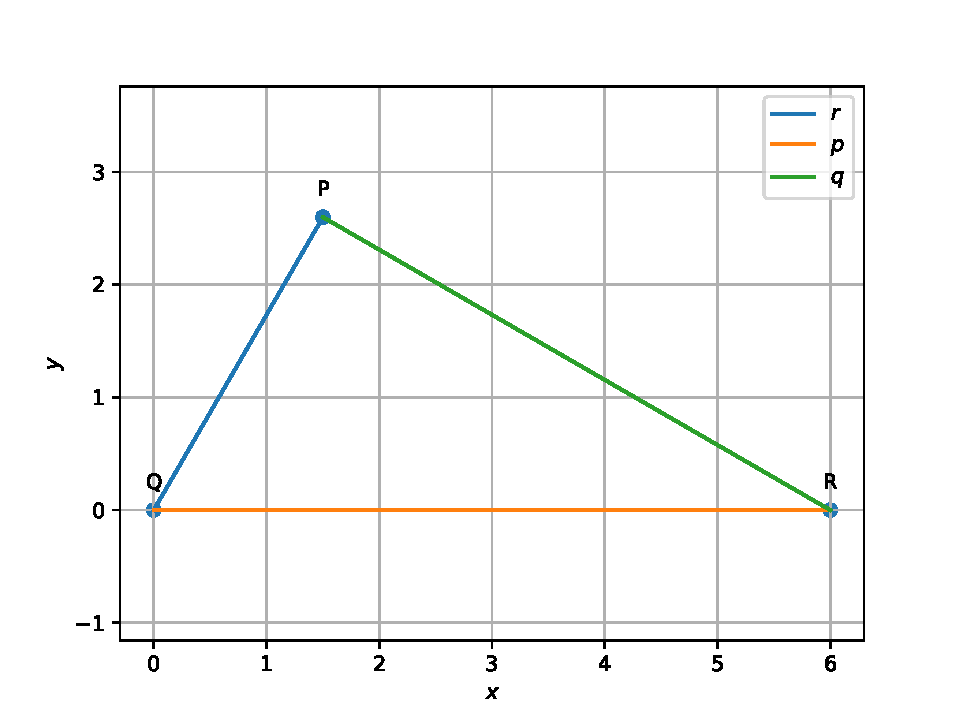
\includegraphics[width=\columnwidth]{chapters/9/11/2/3/figs/line1.pdf}
		\caption{}
		\label{fig:9/11/2/3}
  	\end{figure}
	\solution  Same as Problem 
\ref{chapters/9/11/2/1} with 
\begin{align}
\angle Q = \angle B, QR = a, PR = b, PQ = c
\end{align}
\iffalse

\textbf{Law of Cosines}
\vspace{2mm}\raggedright \\

The law of Cosines relates the length of the triangle to the cosines of one of its angles. It states that, if the length of two sides and the angle between them is known for a triangle, then we can determine the length of the third side. It is given by:
\begin{equation}
\alpha^2=\beta^2+\gamma^2-2\beta\gamma\cos\theta
\end{equation}
%-----------------------------solution---------------------------
\raggedright \textbf{SOLUTION}:\vspace{5mm}\\
\raggedright \textbf{Steps of Construction:}\vspace{2mm}\\
\textbf{Step 1:}\vspace{2mm}\\
Let P,Q and R be the vertices of the triangle  with coordinates.

Given QR length is a=6cm,
So the coordinates of vertices  Q,R and P are :\vspace{2mm}\\
\begin{center}$
{
 Q =\begin{pmatrix}
0 \\
0 
\end{pmatrix} 
\vspace{1mm}
R=\begin{pmatrix}
6 \\
0 
\end{pmatrix} 
\vspace{1mm}
P=\alpha\begin{pmatrix}
cos \theta\\
  sin \theta\\
\end{pmatrix} }
\vspace{1mm}$
\end{center}
Also given the angle is $Q=60^0$,so by finding the coordinates of the other sid
    e we can form a required triangle. \\
 \vspace{2mm}
For the input parameters in Table 1.\\
{\setlength\extrarowheight{2pt}
\begin{center}
\begin{tabular}{|c|c|c|}
	\hline
	\textbf{Symbol}&\textbf{Value}&\textbf{Description}\\
	\hline
	Q&$\begin{pmatrix}
	0\\0\\
	\end{pmatrix} $& Q Point\\
	\hline
	R&$\begin{pmatrix}
	6\\0\\
	\end{pmatrix} $& R Point\\
	\hline
	$\theta$&60$^{\circ}$&$\angle$PQR\\
	\hline
	$\lambda$ & 2 & PR-PQ\\
	\hline
	q&$\alpha$  & PR\\
	\hline
	r &$\gamma$  & PQ\\
	\hline
	p & 6 & QR\\
	\hline
\end{tabular}
%}\\
\\ {Table 1}\\
\end{center}
\vspace{3mm} 
Given that,
\begin{equation}
	\alpha-\gamma=2
\end{equation}
By using the Cosine formula in  $\Delta$PQR \\ 
\begin{equation}
\alpha^2=\beta^2+\gamma^2-2\beta\gamma\cos\theta 
\end{equation}
\vspace{1mm}
\begin{equation}
\alpha^2-\gamma^2=\beta^2-2\beta\gamma\cos\theta
\end{equation}
\vspace{1mm}
\begin{equation}
(\alpha+\gamma)(\alpha-\gamma)=\beta^2-2\beta\gamma\cos\theta
\end{equation}
\vspace{1mm}
\begin{equation}
(\alpha+\gamma)(\lambda)=\beta^2-2\beta\gamma\cos\theta
\end{equation}
\vspace{1mm}
\begin{equation}
\lambda\alpha +\lambda \gamma +2\beta\gamma\cos\theta=\beta^2
\end{equation}
\vspace{1mm}
\begin{equation}
\lambda \alpha +\gamma(\lambda+2\beta\cos\theta)=\beta^2
\end{equation}
\vspace{1mm}
%\begin{center}
%	$0=6^2+\gamma^2 -\alpha^2-2\times \gamma \times 6 \times cos60$\\

%\vspace{5mm}
%\end{center}
%After simplification
%\begin{equation}
%	   4\gamma+\alpha =18
%\end{equation}

\textbf{Step 2:}\vspace{2mm}\\
We know that,\\
\begin{equation}
\vec{A  X = B}
\end{equation}
Using equation (2) and (8),


\begin{equation}
  \begin{pmatrix}
1 & -1\\
\lambda & \lambda+2\beta\cos\theta
\end{pmatrix} 
\begin{pmatrix}
\alpha\\
\gamma
\end{pmatrix} 
=
\begin{pmatrix}
\lambda\\ 
 \beta^2\
\end{pmatrix}
\end{equation}\vspace{2mm}\\
 
After substituting values,
\begin{equation}
  \begin{pmatrix}
1 & -1\\
1 &4
\end{pmatrix} 
\begin{pmatrix}
\alpha\\
\gamma
\end{pmatrix} 
=
\begin{pmatrix}
2\\ 
 18\
\end{pmatrix}
\end{equation}\vspace{2mm}\\


The augmented matrix for the above matrix equation is 
\vspace{3mm}
\begin{equation}
\begin{pmatrix}
  1 & -1 & \vrule & 2\\
  1 & 4  &\vrule & 18
    \end{pmatrix}  
    \end{equation} 
    
  \begin{center}
  $ \xleftrightarrow{\text{$R_2$ $\leftarrow {R_2}-{R_1}$}} $
$\begin{pmatrix}
 1 & -1& \vrule & 2\\
 0 & 5  &\vrule & 16\
  \end{pmatrix}$
  \\
  \end{center}
  
  \begin{center}
$ \xleftrightarrow{\text{$R_2$ $\leftarrow  \frac{1}{5}{R_2}$}} $
$\begin{pmatrix}
 1 & -1 & \vrule & 2\\
  0 & 1  &\vrule & \frac{16}{5}\
  \end{pmatrix}$
  \\
  \end{center}    
  
  \begin{center}
  $ \xleftrightarrow{\text{$R_1$ $\leftarrow  {R_1}+{R_2}$}} $
$\begin{pmatrix}
  1 & 0 & \vrule & \frac{26}{5}\\
  0 & 1  &\vrule & \frac{16}{5}\
  \end{pmatrix}$
  \\
  \end{center}

  \begin{equation}
\implies X = 
   \begin{pmatrix}
   \frac {26}{5}\\ 
   \frac{16}{5}
 \end{pmatrix}
 \end{equation}
Using equation (7) we get ,
\begin{equation}
	\alpha = \frac{26}{5} \vspace{2mm}
\end{equation}
\begin{equation}
	\gamma= \frac{16}{5}\vspace{2mm}
\end{equation}
The vertices of $\Delta$ PQR are \\
\begin{equation}
P= \frac{26}{5} \begin{pmatrix}
cos 60\\
sin 60\\
\end{pmatrix} 
,Q= \begin{pmatrix}
 0\\
 0\\
 \end{pmatrix} 
,R= \begin{pmatrix}
 6\\
 0\\
\end{pmatrix} 
\end{equation} \vspace{2mm}


\textbf{Result} 
\begin{center}
	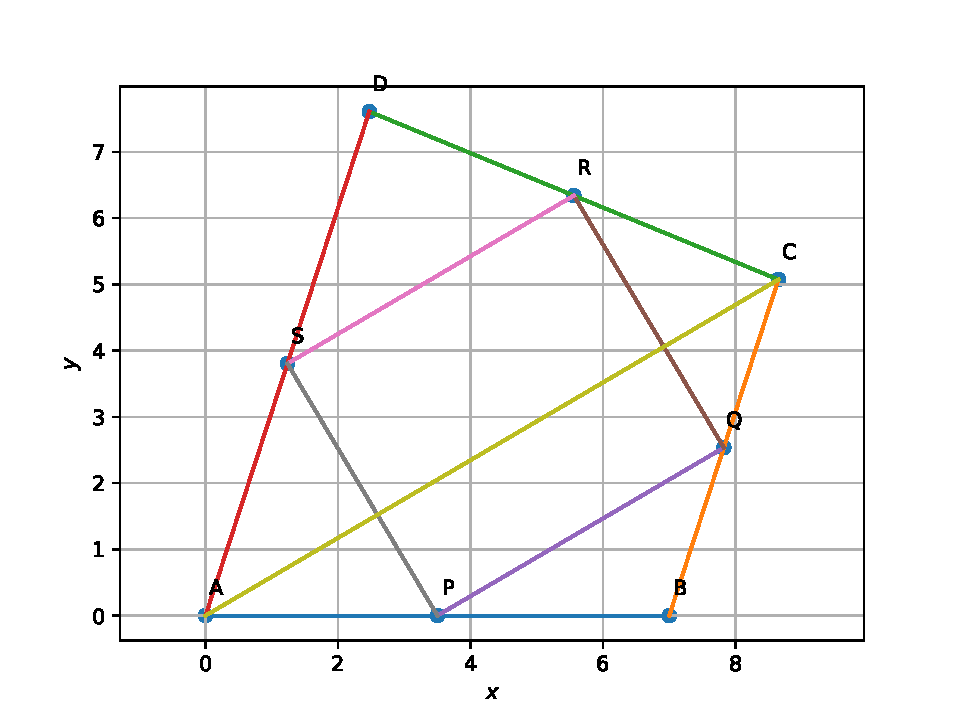
\includegraphics[width=0.4\textwidth]{line1.pdf}
\end{center}\vspace{5mm}

\vspace{4mm}  
\textbf{Implementation}
\begin{center}
\setlength{\arrayrulewidth}{0.5mm}
\setlength{\tabcolsep}{5pt}
\renewcommand{\arraystretch}{3}
    \begin{tabular}{|l|c|}
    \hline 
    \textbf{Equation no} & \textbf{Role} \\ \hline
    1 &  law of Cosines \\ 
    7 & Matrix form of Linear equation  \\
    10 & Length of r\\
    11& Length of q \\
    
    \hline
      \end{tabular}
  \end{center} \vspace{2mm} 



  \vspace{2mm} \textbf{Construction}
\begin{center}
\setlength{\arrayrulewidth}{0.5mm}
\setlength{\tabcolsep}{6pt}
\renewcommand{\arraystretch}{1.5}
    \begin{tabular}{|l|c|}
  \hline 
  \textbf{vertex} & \textbf{coordinates} \\ \hline
P & $ \begin{pmatrix} 
2.6 \\
4.5
\end{pmatrix} $ \\ \hline
   Q & $\begin{pmatrix}
0 \\
0
\end{pmatrix}$   \\\hline
   R & $\begin{pmatrix}
6 \\
0
\end{pmatrix} $\\
   \hline
    \end{tabular}
\end{center}
  
  
 
\raggedright  Download the code \\
https://github.com/Gangagopinath/ASSIGNMENT/tree/
\newline
main/assignment4
}  \end{multicols}
\end{document}
\fi

%
\item 
\label{cons/tri/5}
\iffalse
\documentclass[10pt,a4paper]{report}
%\usepackage[latin1]{inputenc}
\usepackage[utf8]{inputenc}
\usepackage{amsmath}
\usepackage{amsfonts}
\usepackage{amssymb}
\usepackage{graphicx}
\usepackage{multicol}
\usepackage{tabularx}
\usepackage{tikz}
\usetikzlibrary{arrows,shapes,automata,petri,positioning,calc}
\usepackage{hyperref}
\usepackage{tikz}
\usetikzlibrary{matrix,calc}
\usepackage[margin=0.5in]{geometry}
\newcommand{\myvec}[1]{\ensuremath{\begin{pmatrix}#1\end{pmatrix}}}
\let\vec\mathbf
\newenvironment{Figure}
  {\par\medskip\noindent\minipage{\linewidth}}
  {\endminipage\par\medskip}
\begin{document}
%--------------------logo figure-------------------------%
\begin{figure*}[!tbp]
  \centering
  \begin{minipage}[b]{0.4\textwidth}
    
\includegraphics[scale = 0.05]{iitlogo.jpg}
  \end{minipage}
  \hfill
  \vspace{5mm}\begin{minipage}[b]{0.4\textwidth}
\raggedleft  
\includegraphics[scale = 0.10]{nrc.png}\

  \end{minipage}\vspace{0.2cm}
\end{figure*}
%--------------------name & rollno-----------------------
\raggedright \textbf{Name}:\hspace{1mm} Chirag Shah\hspace{3cm} \Large \textbf{Assignment-4}\hspace{2.5cm} % 
\normalsize \textbf{Roll No.} :\hspace{1mm} FWC22053\vspace{1cm}
\begin{multicols}{2}

\textbf{Triangle Law of Vector addition }
\vspace{0.5cm}\raggedright \\
The triangle law of vector addition says that when two vectors are represented as two sides of a triangle with the same order of magnitude and direction, then the magnitude and direction of the resultant vector is represented by the third side of the triangle taken in reverse order..\vspace{3mm} \\ 
\begin{equation}
\vec{R}=\vec{A}+\vec{B} 
\end{equation}
%----------------problem statement--------------%
\raggedright \textbf{Problem Statement:}\vspace{2mm}
\raggedright \\
\fi
	Construct a right triangle whose base is 12cm and sum of its hypotenuse and other side is 18cm.
%	\begin{figure}[!h]
%		\centering
% \includegraphics[width=\columnwidth]{chapters/9/11/2/5/figs/line.png}
%		\caption{}
%		\label{fig:9/11/2/5}
%  	\end{figure}
	\\
	\solution From the given information, let 
\begin{align}
a = 12, \angle B = 90 \degree, b+c = 18
\end{align}
We need to find $b$.  This is similar to Problem 
\ref{chapters/9/11/2/1}.

	\iffalse
\vspace{5mm}
%-----------------------------solution---------------------------
\raggedright \textbf{SOLUTION}:\vspace{2mm}\\
Let A,B and C be the vertices of right triangle with with coordinates $\begin{pmatrix}
0 \\
0 
\end{pmatrix} 
, \begin{pmatrix}
0 \\
0 
\end{pmatrix} 
 and \begin{pmatrix}
0 \\
0 
\end{pmatrix} $
\vspace{1mm} respectively.\vspace{2mm}\\
OB-Base.
AB-Hypotenuse.
OA-Side.\\\vspace{2mm}
%---------given----------------%
\raggedright \textbf{Given}:\vspace{2mm}\\
Since its a right triangle OA $\perp$ OB \\\vspace{2mm}
Since base is 12cm length of OB = 12  \\i.e,\\
\begin{equation}
b= 12 \vspace{2mm}
\end{equation}
Sum of length OA and AB = 18cm \\ i.e,\\
\begin{equation}
a + c= 18 \vspace{2mm}
\end{equation}
%-------------To find ------------------%
\textbf{To Find}\vspace{2mm}\\
The magnitude of a \hspace{2mm} i.e \\ \vspace{2mm}
%--------------steps----------------------%
\textbf{STEP-1}\vspace{2mm}\\
Let k be the unknown point in the vertex A \vspace{2mm}\\
Then coordinates of vertices  O,A and B are :\vspace{2mm}\\
\begin{center}$
\vec{
 O =\begin{pmatrix}
0 \\
0 
\end{pmatrix} 
\vspace{1mm}
B=\begin{pmatrix}
12 \\
0 
\end{pmatrix} 
\vspace{1mm}
A=\begin{pmatrix}
0 \\
k 
\end{pmatrix} }
\vspace{1mm}$
\end{center}

\vspace{3mm} 
We know that a + c= 18 \vspace{2mm}\\
So, Let m=18 
\begin{equation}
   a +c = m \vspace{2mm}
\end{equation}
We know that , \\
\begin{equation}
c^2 = a^2 + b^2 \vspace{2mm}
\end{equation}

\textbf{STEP-2}\vspace{2mm}\\
\begin{equation}\vec{
    O=\begin{pmatrix}
0\\
0
\end{pmatrix} 
    B=\begin{pmatrix}
12\\
0
\end{pmatrix} 
    A=\begin{pmatrix}
0\\
k
 \end{pmatrix} } \vspace{3mm}
\end{equation}
  
By using equation (5)
\begin{center}
    $ c^2 =a^2 + b^2 $ \vspace{2mm}
\end{center}
\begin{equation}
    b^2 = c^2- a^2 \vspace{2mm}
\end{equation}
We know that $c^2- a^2 =  (c-a) (c+a)$\vspace{2mm}\\
Since, $ c+a=m$
\begin{equation}
  b^2 = c-a (m) \vspace{2mm}
\end{equation}
\begin{equation}
 c-a = \frac{b^2}{m}
\end{equation}
And ,
\begin{equation}
 c+a = m \vspace{2mm}
\end{equation}
Using equation (9) and (10),
\begin{equation}
  \begin{pmatrix}
1 & 1\\
1 &-1
\end{pmatrix} 
\begin{pmatrix}
c\\
a
\end{pmatrix} = \begin{pmatrix}
m\\
\frac{b^2}{m}
\end{pmatrix} 
\end{equation}\vspace{2mm}\\

\textbf{STEP-2}\vspace{2mm}\\
Using equation (11) \vspace{2mm}\\
 Let,
\begin{equation}
\vec{P} =\begin{pmatrix}
1 & 1\\
1 &-1
\end{pmatrix} 
\end{equation} \\ \vspace{2mm}
\begin{equation}
  \vec{y} =\begin{pmatrix}
c \\
a
\end{pmatrix} 
\end{equation}  \vspace{2mm}

\begin{equation}
 \vec{Q} = \begin{pmatrix}
x\\
\frac{b^2}{m}
\end{pmatrix} 
\end{equation}\vspace{2mm}
We know that,\\
\begin{equation}
\vec{P  y = Q}
\end{equation}
And,\\
\begin{equation}
\vec{P^{-1} P = I}
\end{equation}
multiplying $P^{-1}$ on both sides in equation (15)\\
\begin{equation}
 \vec{y = P^{-1} Q}
\end{equation}
Using equation (17) we get ,
\begin{equation}
c = 13 \vspace{2mm}
\end{equation}
\begin{equation}
 a = 5 \vspace{2mm}
\end{equation}
The Coordinates of $\vec{A}=\begin{pmatrix}
0\\
k
\end{pmatrix}$  is ,\\
\begin{equation}
 \vec{A}=\begin{pmatrix}
0 \\
5
\end{pmatrix} 
\end{equation}
\textbf{Result} 
\begin{center}
 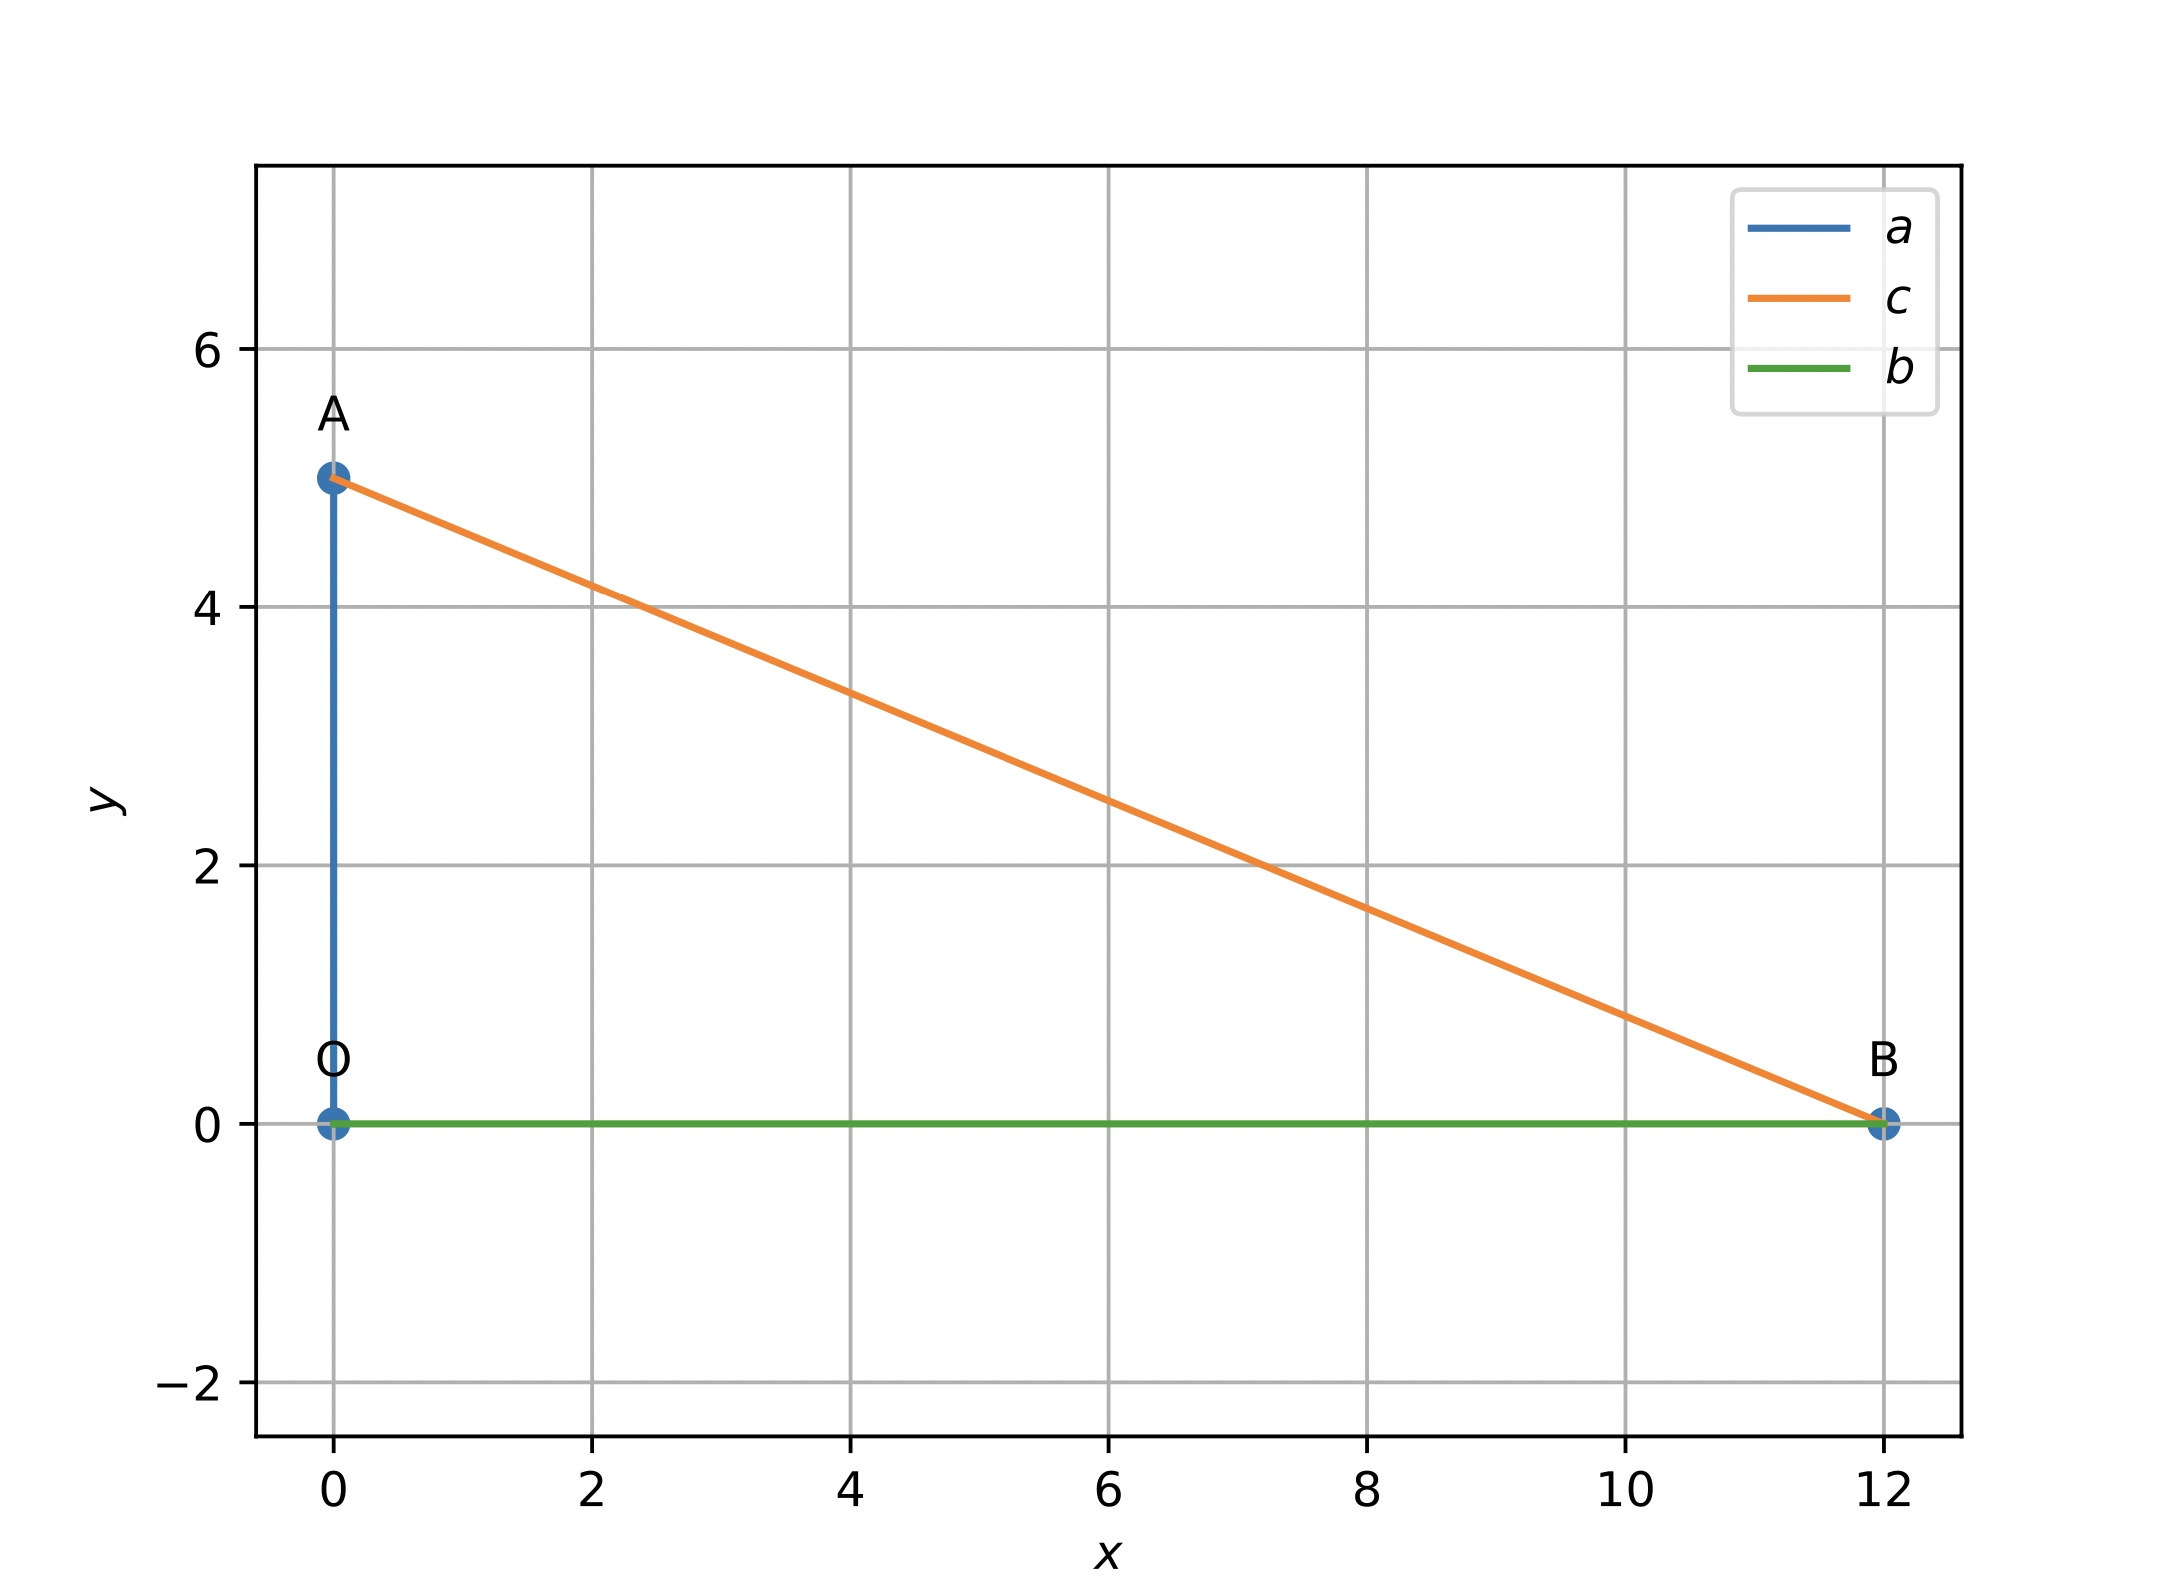
\includegraphics[width=0.5\textwidth]{matrix.jpg}  
 \end{center}\vspace{5mm}
 \vspace{2mm}  
\textbf{implementation}
\begin{center}
\setlength{\arrayrulewidth}{0.5mm}
\setlength{\tabcolsep}{5pt}
\renewcommand{\arraystretch}{3}
    \begin{tabular}{|l|c|}
    \hline 
    \textbf{Equation no} & \textbf{Role} \\ \hline
    5 &  Pythagorean Theorem \\ 
    11 & Matrix form of Linear equation  \\
    16 & Results Identity matrix  \\
    18 & Length of c\\
    19 & Length of a \\
    20 & substituting k=5\\
    \hline
      \end{tabular}
  \end{center} \vspace{2mm}
  
 \vspace{2mm} \textbf{Construction}
\begin{center}
\setlength{\arrayrulewidth}{0.5mm}
\setlength{\tabcolsep}{6pt}
\renewcommand{\arraystretch}{1.5}
    \begin{tabular}{|l|c|}
    \hline 
    \textbf{vertex} & \textbf{coordinates} \\ \hline
   O & $ \begin{pmatrix} 
0 \\
0
\end{pmatrix} $ \\ \hline
    A & $\begin{pmatrix}
0 \\
5
\end{pmatrix}$   \\\hline
    B & $\begin{pmatrix}
12 \\
0
\end{pmatrix} $\\
    \hline
      \end{tabular}
  \end{center}
  
\raggedright  Download the code \\
Github link: \href{https://github.com/chiragshah1244/FWC/blob/main/assignments/assignment-1/code/src/seq.cpp}{Assignment-4}.
  \end{multicols}
\end{document}
\fi

\fi
%
\item Construct a triangle $ABC$ in which $\angle{B}, \angle{C}$ and  $a+b+c=K$ are given.
\label{cons/tri/4}
\\
\solution
\iffalse
\documentclass[10pt,a4paper]{report}
\usepackage[latin1]{inputenc}
\usepackage{amsmath}
\usepackage{amsfonts}
\usepackage{amssymb}
\usepackage{graphicx}
\usepackage{hyperref}
\usepackage{multicol}
\usepackage[margin=0.5in]{geometry}
\usepackage{tikz}
\usepackage[document]{ragged2e}
\usepackage{romannum}
\usetikzlibrary{arrows,shapes.gates.logic.US,shapes.gates.logic.IEC,calc}
\usepackage{titlesec}
\titlespacing{\subsection}{1pt}{\parskip}{3pt}
\titlespacing{\subsubsection}{0pt}{\parskip}{-\parskip}
\titlespacing{\paragraph}{0pt}{\parskip}{\parskip}
\newcommand{\myvec}[1]{\ensuremath{\begin{pmatrix}#1\end{pmatrix}}}



\begin{document}



\begin{multicols}{2}
\raggedright {
\includegraphics[scale=0.06]{IITH logo.jpg}} \vspace{3mm}\\ \raggedleft Name:SHAIK KHAJA MASTAN AHMED\vspace{2mm}\\ \raggedleft Roll No.: FWC22052\vspace{2mm}\\ \raggedleft 19pa1a04e9@vishnu.edu.in \vspace{2mm}\\ \raggedleft Sep 2022 \vspace{5mm}\\

\end{multicols}
\centering \Large \textbf{MATRIX: LINE ASSIGNMENT} \normalsize \vspace{10mm}

\begin{multicols}{2}

\section{Problem:}  
	\begin{figure}[!h]
		\centering
 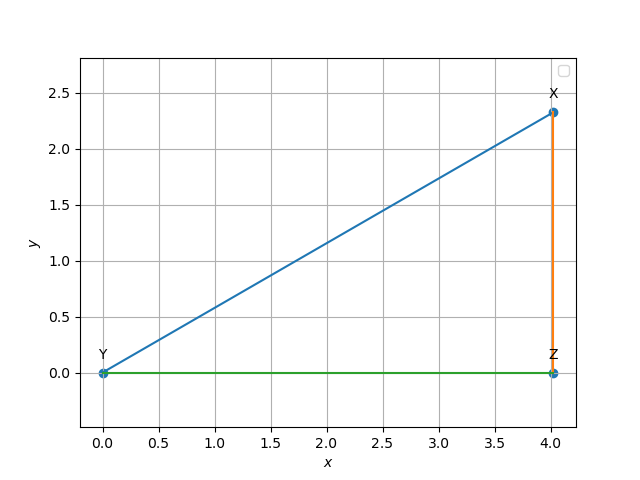
\includegraphics[width=\columnwidth]{chapters/9/11/2/4/figs/line.png}
		\caption{}
		\label{eq:cons/tri/9/11/2/4}
  	\end{figure}
\fi
	From the given information, 
\begin{align}
	a+b+c &= K
	\\
	b\cos C + c \cos B -a &=0
	\\
	b\sin C - c \sin B &=0
\end{align}
resulting in the matrix equation
\begin{align}
	\myvec{
		1 & 1 & 1 
	\\
	\cos C &  \cos B &-1
	\\
	\sin C &-  \sin B & 0
}\myvec{a \\ b \\ c}
= K \vec{e}_1
\end{align}
which can be solved to obtain all the sides.  
\iffalse
	$\triangle ABC$ can then be plotted using
\begin{align}
	\vec{X} = \myvec{a \\ b},
	\vec{Y} = \vec{0},
	\vec{Z} =\myvec{a \\ 0}
\end{align}

\section{Solution: }
\raggedright \textbf{Input Parameters:}\\
\vspace{1mm}
\begin{center}
\begin{tabular}{|c|c|c|}
	\hline
	\textbf{Symbol}&\textbf{Value}&\textbf{Description}\\
	\hline
	XY+YZ+ZX & 11cm & D\\
	\hline 
	$\angle{Z}$ & $90^0$ & Angle at Z \\
	\hline
	$\angle{Y}$ & $30^0$ & Angle at Y \\
	\hline
	
\end{tabular}
\end{center}
\vspace{3mm}



\raggedright Termux Command:\\
               \centering bash rncom.sh (Using Shell)\\
               \vspace{3mm} 

\raggedright \textbf{To Prove:}\\ \vspace{3mm} 
   Given, $\angle{Y}=30^0$, $\angle{Z}=90^0$ and  XY+YZ+ZX = Dcm.\\ \vspace{1mm}
   if $\angle{Y}=30^0$ and $\angle{Z}=90^0$ then $\angle{X}=60^0$\\
   Let us consider the coordinates of Y are X0,Y0 be $\begin{pmatrix}
  0\\
  0 \\
 \end{pmatrix}$% 
 \vspace{1mm} \\ Let 'z' be the distance between X and Y.
 \vspace{1mm} \\ Let the coordinates of X be X1,Y1 respectively.
  \\ \centering i.e., X = z$\begin{pmatrix}
  cos \theta\\
  sin \theta \\
 \end{pmatrix}$% 
 \vspace{2mm}
  \\ \raggedright And the coordinates of Z be X2,Y2 respectively.
  \\ \centering i.e., Z = z$\begin{pmatrix}
  cos \theta\\
  0 \\
 \end{pmatrix}$%
 \vspace{2mm}  \\So, by finding the values of coordinates of the all sides we can form a required triangle. \\
\vspace{2mm}
\raggedright \textbf{Finding the Coordinates: } \\
        \raggedright Given that XY+YZ+ZX=D. \frenchspacing \\
        \raggedright i.e., $||X-Y||$ + $||Y-Z||$ + $||Z-X||$ =D. \\ \vspace{1mm}
 $\implies$ z + zcos$\theta$+ zsin$\theta$ =D\\  
	\begin{center}	
	$\implies$ z = $\frac{D}{1+cos\theta+sin\theta}$
	\end{center}
\centering By solving we get 'z' , [$\because$ $\theta=30^0$ and D=11cm].\\ \vspace{2mm}
 $\therefore$ \text{z = 4.64} .\\ 
\raggedright Calculating the required vertices: \\ \vspace{2mm}
\centering X = z$\begin{pmatrix} 
  cos \theta\\
  sin \theta\\
 \end{pmatrix}$ =4.64 $\begin{pmatrix} 
  cos30^0\\
  sin30^0\\
 \end{pmatrix}$ = $\begin{pmatrix}
                 4.02\\
                 2.32\\
              \end{pmatrix}$ \\ \vspace{2mm}
\centering Z = z$\begin{pmatrix} 
  cos \theta\\
  0\\
 \end{pmatrix}$ = 4.64 $\begin{pmatrix} 
  cos30^0\\
  0\\
 \end{pmatrix}$ = $\begin{pmatrix}
                  4.02\\
                  0\\
              \end{pmatrix}$\\ \vspace{2mm}
\raggedright $\therefore$ The vertices of the required $\Delta$XYZ are:\\ \vspace{2mm}
\centering X= $\begin{pmatrix}
                 4.02\\
                 2.32\\
              \end{pmatrix}$%
              , Y= $\begin{pmatrix}
                 0\\
                 0\\
              \end{pmatrix}$% 
               , Z= $\begin{pmatrix}
                  4.02\\
                  0\\
              \end{pmatrix}$% 
 \vspace{3mm}             
\\
\textbf{The below python code realizes construction:}\\
https://github.com/19pa1a04e9/FWC-IITH/tree/main/Assignment-1/MATRICES/Line/line.py
  
 \section{Plot:}
 	\begin{center}
  \includegraphics[scale=0.55]{line.png}
  	\end{center}
  


  



\vspace{3cm}

\end{multicols}

\end{document}
\fi



\end{enumerate}



\chapter{Linear Forms}
\section{Two Dimensions}

%\renewcommand{\theequation}{\theenumi}
%\begin{enumerate}[label=\arabic*.,ref=\theenumi]
\begin{enumerate}[label=\thesection.\arabic*.,ref=\thesection.\theenumi]
%\begin{enumerate}
%\numberwithin{equation}{enumi}
\item The equation of a line  is given by  
\begin{align}
	\label{eq:normal_line}
   \vec{n}^{\top}\vec{x} = c
\end{align}
		where $\vec{n}$ is the normal vector of the line.
	\item The equation of a line with normal vector $\vec{n}$ and passing through a point $\vec{A}$ 
		is given by 
\begin{align}
    \label{eq:line_norm_eq}
%	\label{eq:normal_line_pt}
	\vec{n}^{\top}\brak{\vec{x}-\vec{A}} =0 
\end{align}
\item The equation of a line $L$ is also given by  
\begin{align}
	\label{eq:normal_line_orig}
   \vec{n}^{\top}\vec{x}  = 
	\begin{cases}
		0  & \vec{0} \in L
		 \\
		1 & \text{otherwise}
	\end{cases}
\end{align}
\item Points $\vec{A}, \vec{B}, \vec{C}$ are collinear if  
\begin{align}
	\label{eq:normal_line-collinear}
	\rank	\myvec{ \vec{B}-\vec{A} &\vec{C}-\vec{A}} < 2
\end{align}

	\begin{proof}
		From 
	\eqref{eq:normal_line}, 
\begin{align}
	\vec{n}^{\top}\vec{A} &= c
	\\
	\vec{n}^{\top}\vec{B} &= c
	\\
	\vec{n}^{\top}\vec{C} &= c
\end{align}
which can be expressed as
\begin{align}
	\myvec{\vec{A} &\vec{B} &\vec{C}}^{\top}\vec{n} = c\myvec{1 \\ 1 \\ 1}
\end{align}
The above set of equations are consistent if 
\begin{align}
	\rank	\myvec{1 & 1 & 1 \\ \vec{A} &\vec{B} &\vec{C}} < 3
	\\
	\implies 
	\rank	\myvec{1 & 0 & 0 \\ \vec{A} &\vec{B}-\vec{A} &\vec{C}-\vec{A}} < 3
\end{align}
using the fact that row rank = column rank.  The above condition can then be expressed as
	\eqref{eq:normal_line-collinear}.


	\end{proof}
%	\item The equation of a line with normal vector $\vec{n}$ and passing through a point $\vec{A}$ 
%		is given by 
%\begin{align}
%    \label{eq:line_norm_eq-pt}
%%	\label{eq:normal_line_pt}
%	\vec{n}^{\top}\brak{\vec{x}-\vec{A}} =0 
%\end{align}
\item The parametric equation of a line  is given by  
\begin{align}
	\label{eq:dir_line}
	\vec{x} = \vec{A} + \lambda \vec{m}
\end{align}
		where $\vec{m}$ is the direction vector of the line and $\vec{A}$ is any point on the line.
  \item Let $\vec{A}$ and $\vec{B}$ be two points on a straight line and let $\vec{P}= \myvec{p_1\\p_2}$ be any point on it. If $p_2$ is known, then 
  \begin{align}
	  \vec{P}  &=	  \vec{A} + \frac{p_2 -\vec{e}_2^{\top}  \vec{A} }{\vec{e}_2^{\top}\brak{\vec{B} -\vec{A} }}\brak{\vec{B} -\vec{A} }
	  \label{eq:line-3pt}
  \end{align}
  \solution The equation of the line can be expressed in parametric from as 
  \begin{align}
	  \vec{x}  &=	  \vec{A} + \lambda \brak{\vec{B} -\vec{A} }
	  \\
	  \implies 
	  \vec{P}  &=	  \vec{A} + \lambda \brak{\vec{B} -\vec{A} }
	  \\
	  \implies 	   \vec{e}_2^{\top}\vec{P}  &=	\vec{e}_2^{\top}  \vec{A} + \lambda \vec{e}_2^{\top}\brak{\vec{B} -\vec{A} }
	  \\
	 \implies p_2 &=\vec{e}_2^{\top}  \vec{A} + \lambda \vec{e}_2^{\top}\brak{\vec{B} -\vec{A} }
	 \\
	  \text{or, } \lambda &= \frac{p_2 -\vec{e}_2^{\top}  \vec{A} }{\vec{e}_2^{\top}\brak{\vec{B} -\vec{A} }}
  \end{align}
	  yielding \eqref{eq:line-3pt}.
	\item The distance from a point $\vec{P}$ to the line  in 
	\eqref{eq:normal_line}
	is given by 
\begin{align}
  \label{conics/30/lemma}
%	\label{eq:line_dist_2d}
	d = \frac{\abs{   \vec{n}^{\top}\vec{P}-c }}{\norm{\vec{n}}}	
\end{align}
		\solution Without loss of generality, let $\vec{A}$ be the foot of the perpendicular from $\vec{P}$ to the line in 
	\eqref{eq:dir_line}.  The equation of the normal to 
	\eqref{eq:normal_line} can then be expressed as 
\begin{align}
	\label{eq:dir_line_normal_dist}
	\vec{x} &= \vec{A} + \lambda \vec{n}
	\\
	\implies 
	\vec{P}- \vec{A} &=  \lambda \vec{n}
	\label{eq:dir_line_normal_dist_pa}
\end{align}
$\because \vec{P}$ lies on 
		\eqref{eq:dir_line_normal_dist}.
From the above, the desired distance can be expressed as 
\begin{align}
d = 	\norm{\vec{P}- \vec{A}}= \abs{\lambda} \norm{\vec{n}}
	\label{eq:dir_line_normal_dist_pa_d}
\end{align}
From 
	\eqref{eq:dir_line_normal_dist_pa},
\begin{align}
	\vec{n}^{\top}
	\brak{\vec{P}- \vec{A}} &=  \lambda \vec{n}^{\top}\vec{n} = \lambda\norm{\vec{n}}^2
	\\
	\implies \abs{\lambda}&= \frac{\abs{\vec{n}^{\top}
	\brak{\vec{P}- \vec{A}}}}{\norm{\vec{n}}^2} 
\end{align}
	Substituting the above in \eqref{eq:dir_line_normal_dist_pa_d} and using 
	the fact that 
\begin{align}
   \vec{n}^{\top}\vec{A} = c
\end{align}
from 	\eqref{eq:normal_line}, yields 
  \eqref{conics/30/lemma}
%	\eqref{eq:line_dist_2d}.

	\item The distance from the origin to the line  in 
	\eqref{eq:normal_line}
	is given by 
\begin{align}
	\label{eq:dist_line_2d_orig}
	d = \frac{\abs{   c }}{\norm{\vec{n}}}	
\end{align}
\item The distance between the parallel lines 
\begin{align}
	\label{eq:parallel_lines}
	\begin{split}
		\vec{n}^{\top}\vec{x} &= c_1
		\\
		\vec{n}^{\top}\vec{x} &= c_2
	\end{split}
\end{align}
is given by 
\begin{align}
	\label{eq:dist_lines_2d}
	d = \frac{\abs{   c_1-c_2 }}{\norm{\vec{n}}}	
\end{align}
\item The equation of the line perpendicular to 
	\eqref{eq:normal_line}
		and passing through the point $\vec{P}$ is given by 
\begin{align}
	\vec{m}^{\top}\brak{\vec{x}-\vec{P}}  = 0
\end{align}
\item The foot of the perpendicular from $\vec{P}$ to the line in 
	\eqref{eq:normal_line}
	is given by 
\begin{align}
	\label{eq:normal_line_foot}
	\myvec{ \vec{m} & \vec{n}}^{\top}\vec{x}= \myvec{\vec{m}^{\top}\vec{P}\\ c }  
\end{align}
% 
\solution From
	\eqref{eq:normal_line} and 
\eqref{eq:line_norm_eq}
%	\eqref{eq:normal_line_pt} 
the foot of the perpendicular satisfies the equations 
\begin{align}
	\vec{n}^{\top}\vec{x} &= c
	\\
	\vec{m}^{\top}\brak{\vec{x}-\vec{P} }&=0 
\end{align}
where $\vec{m}$ is the direction vector of the given line.  Combining the above into a matrix equation results in 
	\eqref{eq:normal_line_foot}.
\item The equations of the angle bisectors of  the lines 
	\label{prob:ang-bisect}
\begin{align}
	\vec{n}_1^{\top}\vec{x} &= c_1
	\\
	\vec{n}_2^{\top}\vec{x} &= c_2
\end{align}
are given by 
\begin{align}
	\frac{\vec{n}_1^{\top}\vec{x} - c_1}{\norm{\vec{n}_1}}
	= \pm
	\frac{\vec{n}_2^{\top}\vec{x} - c_2}{\norm{\vec{n}_2}}
\end{align}
\begin{proof}
Any point on the angle bisector is equidistant from the lines.  
\end{proof}
\item In $\triangle ABC$, the direction of the angle bisector of $A$ is given by 
\begin{align}
\vec{m} = \vec{B}+\vec{C}-2\vec{A}
	\label{eq:ang-bisect-dir}
\end{align}
\solution
Since the direction vectors of $AB$ and $AC$ are 
\begin{align}
 \vec{B}-\vec{A}, \vec{C}-\vec{A}
\end{align}
using the parallelogram law, we obtain
	\eqref{eq:ang-bisect-dir}.
	\item The perpendicular bisector of $BC$ is given by 
		\begin{align}
			\brak{\vec{B}-\vec{C}}^{\top} \vec{x} = \frac{\norm{\vec{B}}^2 -\norm{\vec{C}}^2}{2}
			\label{prob:perp-bisect}
		\end{align}
		\solution The perpendicular bisector passes through the mid point 
\begin{align}
	\frac{\vec{B}+ \vec{C}}{2}
\end{align}
and has normal vector 
\begin{align}
	\vec{B}- \vec{C}
\end{align}
Hence, the equation of the perpendicular bisector is 
\begin{align}
	\brak{\vec{B}- \vec{C}}^{\top}\sbrak{\vec{x}- \frac{\vec{B}+ \vec{C}}{2}} &= 0
\end{align}
yielding
			\eqref{prob:perp-bisect}.

		mid point of $BC$ is 

%\item ({\em Reflection }) Assuming that straight lines work as a plane mirror for a point, find the image of the point $\vec{P}=\myvec{1\\2}$ in the line 
%%
%\begin{align}
%L: \quad \myvec{1 & -3}\vec{x}  = -4.
%\end{align}
%\solution From the given equation, the line parameters are
%\begin{align}
%\vec{n} = \myvec{1 \\ -3}, c =  -4, \vec{m} = \myvec{3 \\ -1}
%\end{align}
%
%Let $\vec{R}$ be the reflection of $\vec{P}$ such that $PR$ bisects the line $L$ at $\vec{Q}$. Then $\vec{Q}$ bisects $PR$.  
%This leads to the following equations
%\begin{align}
%\label{eq:reflect_bisect}
%2\vec{Q} &= \vec{P}+\vec{R}
%\\
%\label{eq:reflect_Q}
%\vec{n}^{\top}\vec{Q} &= c \quad \because \vec{Q} \text{ lies on the given line}
%\\
%\label{eq:reflect_R}
%\vec{m}^{\top}\vec{R} &= \vec{m}^{\top}\vec{P} \quad \because \vec{m}\perp \vec{P} - \vec{R}
%\end{align}
%%
%%where 
%%$\vec{m}$ is the direction vector of $L$.  
%From \eqref{eq:reflect_bisect} and \eqref{eq:reflect_Q},
%\begin{align}
%\label{eq:reflect_bisectQ}
%\vec{n}^{\top}\vec{R}  &= 2c - \vec{n}^{\top}\vec{P}
%\end{align}
%%
%From \eqref{eq:reflect_bisectQ} and \eqref{eq:reflect_R},
%\begin{align}
%\label{eq:reflect_bisectQR}
%\myvec{\vec{m} & \vec{n}}^T\vec{R} &= \myvec{\vec{m} & -\vec{n}}^T\vec{P}+ \myvec{0 \\ 2c}
%\end{align}
%%
%Letting 
%\begin{align}
%\label{eq:reflect_mat}
%\vec{V}=  \myvec{\vec{m} & \vec{n}}
%\end{align}
%with the condition that $\vec{m},\vec{n}$ are orthonormal, i.e.
%\begin{align}
%\label{eq:reflect_ortho}
%\vec{V}^T\vec{V}=  \vec{I}
%\end{align}
%%
%Noting that 
%\begin{align}
%\label{eq:reflect_trans}
%\myvec{\vec{m} & -\vec{n}} &= \myvec{\vec{m} & \vec{n}} \myvec{1 & 0 \\ 0 & -1},
%\end{align}
%\eqref{eq:reflect_bisectQR} can be expressed as
%%
%\begin{align}
%\label{eq:reflect_}
%\vec{V}^T\vec{R} &=  \sbrak{\vec{V}\myvec{1 & 0 \\ 0 & -1}}^T\vec{P}+\myvec{0 \\ 2c}
%\\
%\implies \vec{R} &= \sbrak{\vec{V}\myvec{1 & 0 \\ 0 & -1}\vec{V}^{-1}}^T\vec{P}+ \vec{V}\myvec{0 \\ 2c}
%\\
% &=\vec{V}\myvec{1 & 0 \\ 0 & -1}\vec{V}^T \vec{P}+2c \vec{n}
%\label{eq:reflect_mat_final}
%\end{align}
%upon substituting from \eqref{eq:reflect_mat} in \eqref{eq:reflect_mat_final}.
%It can be verified that 
%%\item Show that, for any $\vec{m},\vec{n}$, 
%the reflection is also given by
%\begin{align}
%%\label{eq:reflect_bisect}
%\vec{R} &= \myvec{\vec{m} & \vec{n}}\myvec{1 & 0 \\ 0 & -1}\myvec{\vec{m} & \vec{n}}^T \vec{P}+2c \vec{n}
%\\
% &= \myvec{\vec{m} & -\vec{n}}\myvec{\vec{m}^T \\ \vec{n}^T} \vec{P}+2c \vec{n}
%\\
%\implies \vec{R}&= \brak{\vec{m}\vec{m}^T-\vec{n}\vec{n}^T}\vec{P} + 2c \vec{n} 
%\label{eq:reflect_orth_vec}
%\end{align}
%If $\vec{m}, \vec{n}$ are not orthonormal, \eqref{eq:reflect_orth_vec}
%can be expressed as
%\begin{align}
% \frac{\vec{R}}{2}= \frac{\vec{m}\vec{m}^T-\vec{n}\vec{n}^T}{\vec{m}^T\vec{m}+\vec{n}^T\vec{n}}\vec{P} + c \frac{\vec{n}}{\norm{\vec{n}}^2}
%\label{eq:reflect_non_orth_vec}
%\end{align}
%

\end{enumerate}

\section{Three Dimensions}

%\renewcommand{\theequation}{\theenumi}
%\begin{enumerate}[label=\arabic*.,ref=\theenumi]
\begin{enumerate}[label=\thesection.\arabic*.,ref=\thesection.\theenumi]
%\begin{enumerate}
%\numberwithin{equation}{enumi}
%\item The area of a triangle with vertices $\vec{A}, \vec{B}, \vec{C}$ is given by 
%\begin{align}
%  \label{eq:area3d}
% \frac{1}{2} \norm{\brak{\vec{A} - \vec{B}} \times \brak{\vec{A} - \vec{C}}}
%\end{align}

\item Points $\vec{A}, \vec{B}, \vec{C}$ are on a line if 
\begin{align}
  \label{eq:line_rank}
  \text{rank}\myvec{\vec{A} \\ \vec{B} \\ \vec{C} }  = 1
\end{align}
\item Points $\vec{A}, \vec{B}, \vec{C}, \vec{D}$ form a paralelogram if 
\begin{align}
  \label{eq:parallelgm_rank}
  \text{rank}\myvec{\vec{A} \\ \vec{B} \\ \vec{C} \\ \vec{D}  }  = 1, 
  \text{rank}\myvec{\vec{A} \\ \vec{B} \\ \vec{C} }  = 2
\end{align}
\item The equation of a line  is given by  
	\eqref{eq:dir_line}
	\item The equation of a plane is given by
	\eqref{eq:normal_line}
	\item The distance from the origin to the line  in 
	\eqref{eq:normal_line}
	is given by 
	\eqref{eq:dist_line_2d_orig}
\item The distance from a point $\vec{P}$  to the line in 
	\eqref{eq:dir_line} is given by 
\begin{align}
	\label{dist_3d_def_final}
		d = \norm{\vec{A} -\vec{P}}^2 - \frac{\cbrak{\vec{m}^{\top}\brak{\vec{A}-\vec{P} 
	}}^2}{\norm{\vec{m}}^2}
%	d =\norm{\vec{A}  -\vec{P}
% -\frac{\vec{m}^{\top}\brak{\vec{A} 
%			-\vec{P}}}
%			{ \norm{\vec{m}}^2}
%	\vec{m}}
		\end{align}
		\solution
%		\solution{\title{Solution:}
\begin{align}
	\label{dist_3d_def}
	d\brak{\lambda } &=\norm{\vec{A} + \lambda \vec{m}-\vec{P}}
	\\
\implies 	d^2\brak{\lambda } &=\norm{\vec{A} + \lambda \vec{m}-\vec{P}}^2
\end{align}
which can be simplified to obtain 
	\begin{multline}
d^2\brak{\lambda } =\lambda^2 \norm{\vec{m}}^2+2\lambda \vec{m}^{\top}\brak{\vec{A} 
		-\vec{P}}
		\\
		+\norm{\vec{A} -\vec{P}}^2
	\end{multline}
which is of the form 
\begin{align}
	\label{dist_3d_def_quad}
	d^2\brak{\lambda } &=a \lambda^2 + 2b\lambda +c
	\\
	&=a \cbrak{\brak{\lambda+ \frac{b}{a}}^2 +\sbrak{\frac{c}{a}-\brak{\frac{b}{a}}^2 }}
\end{align}
with 
\begin{align}
	\label{dist_3d_def_quad_abc}
	a = \norm{\vec{m}}^2, b = \vec{m}^{\top}\brak{\vec{A} 
		-\vec{P}}, c = 
		\norm{\vec{A} -\vec{P}}^2
\end{align}
which can be expressed as 
%		\begin{multline}
%			d^2\brak{\lambda } =\norm{\vec{m}}^2\brak{\lambda + \frac{\vec{m}^{\top}\brak{\vec{A}-\vec{P} }}{\vec{m}}^2}}^2 +2\lambda \vec{m}^{\top}\brak{\vec{A} 
%			-\vec{P}}
%			\\
%			+\norm{\vec{A} -\vec{P}}^2
%		\end{multline}
		From the above, $d^2\brak{\lambda}$ is smallest when upon substituting from 
	\eqref{dist_3d_def_quad_abc}
\begin{align}
	\label{dist_3d_def_quad_small}
	\lambda+ \frac{b}{2a} &= 0 \implies \lambda = - \frac{b}{2a}
	\\
	&= -\frac{\vec{m}^{\top}\brak{\vec{A} 
			-\vec{P}}}
			{ \norm{\vec{m}}^2}
	%		\label{dist_3d_lam}
\end{align}
and consequently, 
\begin{align}
	d_{\min}\brak{\lambda } &=a \brak{\frac{c}{a}-\brak{\frac{b}{a}}^2 } 
	\\
	&=c - \frac{b^2}{a }
\end{align}
yielding
	\eqref{dist_3d_def_final} after substituting from 
	\eqref{dist_3d_def_quad_abc}.
%From 	\eqref{dist_3d_def} and \eqref{dist_3d_lam}, 
%	\eqref{dist_3d_def} is obtained.
\item The distance between the parallel planes 
	\eqref{eq:parallel_lines}
	is given by 
	\eqref{eq:dist_lines_2d}.
\item The plane 
		\begin{align}
		\vec{n}^{\top}
			\vec{x} = c
			\label{eq:plain_contain}
		\end{align}
		contains the line 
		\begin{align}
			\vec{x} = \vec{A}+\lambda \vec{m}
			\label{eq:line_contain}
		\end{align}
		if 
		\begin{align}
		\vec{m}^{\top}\vec{n} = 0
			\label{eq:line_plain_contain}
		\end{align}
		\solution Any point on the line 
			\eqref{eq:line_contain}
			should also satisfy 
			\eqref{eq:plain_contain}.  Hence, 
		\begin{align}
			\vec{n}^{\top}\brak{\vec{A}+\lambda \vec{m}} &= \vec{n}^{\top}\vec{A}=c
		\end{align}
		which can be simplified to obtain
			\eqref{eq:line_plain_contain}
		\item The foot of the perpendicular from a point $\vec{P}$ to the plane 
		\begin{align}
			\vec{n}^{\top}\vec{x} =c
		\end{align}
		is given by 
\begin{align}
	\vec{x} &= \vec{P} + \frac{c - \vec{n}^{\top}\vec{P}}{\norm{\vec{n}}^2}
\vec{n}
	\label{eq:foot_perp_pt_plane}
\end{align}
		\\
		\solution The equation of the line perpendicular to the given plane and passing through $\vec{P}$ is 
		\begin{align}
			\vec{x} = \vec{P} + \lambda 	\vec{n}
		\end{align}
		From 
	\eqref{eq:dir_line_plane_isect}, the intersection of the above line with the given plane is 
	\eqref{eq:foot_perp_pt_plane}.
	\iffalse
\begin{align}
	\vec{x} &= \vec{P} + \frac{c - \vec{n}^{\top}\vec{P}}{\norm{\vec{n}}^2}
\vec{n}
	\label{eq:foot_perp_pt_plane}
\end{align}
\fi
\item The image of a point $\vec{P}$ with respect to the plane 
		\begin{align}
			\vec{n}^{\top}\vec{x} =c
		\end{align}
		is given by 
		\begin{align}
			\vec{R} &=
	  \vec{P} + 2\frac{c - \vec{n}^{\top}\vec{P}}{\norm{\vec{n}}^2}
			\label{eq:image_pt_plane}
		\end{align}
		\solution Let $\vec{R}$ be the desired image.  Then, subtituting the expression for the  foot of the perpendicular from $\vec{P}$ to the given plane using 
	\eqref{eq:foot_perp_pt_plane},
		\begin{align}
			\frac{\vec{P}+\vec{R}}{2} &=
	  \vec{P} + \frac{c - \vec{n}^{\top}\vec{P}}{\norm{\vec{n}}^2}
		\end{align}
		\item Let a plane pass through the points $\vec{A},\vec{B}$ and be perpendicular to the plane 
		\begin{align}
		\vec{n}^{\top}\vec{x} =c 
			\label{eq:plane_3d_2pt_perp_given}
		\end{align}
		Then the equation of this plane is given by 
		\begin{align}
		\vec{p}^{\top}\vec{x} = 1
			\label{eq:plane_3d_2pt}
		\end{align}
		where
		\begin{align}
			\vec{p} = 		\myvec{\vec{A} & \vec{B} & \vec{n}}^{-\top}  \myvec{1 \\ 1 \\ 0}
			\label{eq:plane_3d_2pt_perp_norm}
		\end{align}
	\solution From the given information, 
		\begin{align}
			\vec{p}^{\top}\vec{A} &=d 
			\\
			\vec{p}^{\top}\vec{B} &=d 
			\\
			\vec{p}^{\top}\vec{n} &= 0
			\label{eq:plane_3d_2pt_perp_system}
		\end{align}
		$\because$ the normal vectors to the two planes will also be perpendicular.  The system of equations in 
			\eqref{eq:plane_3d_2pt_perp_system}
			can be expressed as the matrix equation
		\begin{align}
			\myvec{\vec{A} & \vec{B} & \vec{n}}^{\top}\vec{p} = d\myvec{1 \\ 1 \\ 0}
			\label{eq:plane_3d_2pt_perp_system_temp}
		\end{align}
		which yields 
			\eqref{eq:plane_3d_2pt_perp_norm}
			upon normalising with $d$.
		\item The intersection of the line represented by 
	\eqref{eq:dir_line}
	with the plane represented by 
	\eqref{eq:normal_line}
	is given by 
\begin{align}
	\label{eq:dir_line_plane_isect}
	\vec{x} &= \vec{A} + \frac{c - \vec{n}^{\top}\vec{A}}{\vec{n}^{\top}\vec{m}}
\vec{m}
\end{align}
\solution From 
	\eqref{eq:dir_line}
	and 
	\eqref{eq:normal_line},
\begin{align}
	\vec{x} &= \vec{A} + \lambda \vec{m}
	\\
	\vec{n}^{\top}\vec{x} &= c
	\\
	\implies 
	\vec{n}^{\top}\brak{\vec{A} + \lambda \vec{m}}&= c
	\label{eq:dir_line_plane_inter}
\end{align}
which can be simplified to obtain
\begin{align}
	\vec{n}^{\top}\vec{A} + \lambda 	\vec{n}^{\top}\vec{m}&= c
	\\
	\implies \lambda &= \frac{c - \vec{n}^{\top}\vec{A}}{\vec{n}^{\top}\vec{m}}
\end{align}
Substituting the above in 
	\eqref{eq:dir_line_plane_inter}
	yields
	\eqref{eq:dir_line_plane_isect}.
\item The foot of the perpendicular from the point $\vec{P}$ to the line  represented by 
	\eqref{eq:dir_line}
	is given by 
\begin{align}
	\label{eq:plane_line_foot_ans}
	\vec{x} &= \vec{A} + \frac{ \vec{m}^{\top}\brak{\vec{P} - \vec{A}}}{\norm{\vec{m}}^2}
\vec{m}
\end{align}
\solution  Let the equation of the line be 
\begin{align}
	\label{eq:dir_line_foot}
	\vec{x} &= \vec{A} + \lambda \vec{m}
\end{align}
	The equation of the plane perpendicular to the given line passing through $\vec{P}$ is given by
\begin{align}
	\label{eq:plane_line_foot}
	\vec{m}^{\top}\brak{\vec{x}-\vec{P}}  &= 0
	\\
	\implies \vec{m}^{\top}\vec{x}  &= \vec{m}^{\top}\vec{P}
\end{align}
The desired foot of the perpendicular is the intersection of 
	\eqref{eq:dir_line_foot} with 
	\eqref{eq:plane_line_foot}
	which can be obtained from 
	\eqref{eq:dir_line_plane_isect}
	as 
	\eqref{eq:plane_line_foot_ans}
\item The foot of the perpendicular from a point $\vec{P}$ to a plane is $\vec{Q}$.  The equation of the plane is given by 
\begin{align}
	\label{eq:plane_foot_perp}
	\brak{\vec{P}-\vec{Q}}^{\top}\brak{\vec{x}-\vec{Q}} = 0
\end{align}
	\solution  The normal vector to the plane is given by 
\begin{align}
	\vec{n}= \vec{P}-\vec{Q} 
\end{align}
	Hence, the equation of the plane is
	\eqref{eq:plane_foot_perp}.
\item Let $\vec{A}, \vec{B}, \vec{C}$ be  points on a plane.  The equation of the plane is then given by 	
\begin{align}
	\myvec{	\vec{A} & \vec{B}& \vec{C}}^{\top} \vec{n}= \myvec{1\\1\\1}
	\label{eq:plane_3pt}
\end{align}
\solution Let the equation of the plane be 
\begin{align}
	\vec{n}^{\top}	\vec{x} &= 1
\end{align}
Then 
\begin{align}
	\vec{n}^{\top}	\vec{A} &= 1
	\\
	\vec{n}^{\top}	\vec{B} &= 1
	\\
	\vec{n}^{\top}	\vec{C} &= 1
\end{align}
which can be combined to obtain 
	\eqref{eq:plane_3pt}.
\item The lines 
    \begin{align}
        \vec{x} = \vec{x_1} + \lambda_1\vec{m_1} \label{eq:chapters/12/11/2/16/L1-gen} \\
        \vec{x} = \vec{x_2} + \lambda_2\vec{m_2} \label{eq:chapters/12/11/2/16/L2-gen}
    \end{align}
    intersect if
    \begin{align}
    %    \lambda_1\vec{m_1} - \lambda_2\vec{m_2} &= \vec{x_2} - \vec{x_1} \\
       \vec{M}\bm{\lambda} &= \vec{x_2} - \vec{x_1}
        \label{eq:chapters/12/11/2/16/intersect-cond}
    \end{align}
    where
    \begin{align}
        \vec{M} \triangleq \myvec{\vec{m_1} & \vec{m_2}} \label{eq:chapters/12/11/2/16/M-def} \\
        \bm{\lambda} \triangleq \myvec{\lambda_1\\-\lambda_2}
        \label{eq:chapters/12/11/2/16/lambda-def}
    \end{align}
\item 
    \iffalse
    Let 
    \begin{align}
        \vec{x} = \vec{x_1} + \lambda_1\vec{m_1} \label{eq:chapters/12/11/2/16/L1-gen} \\
        \vec{x} = \vec{x_2} + \lambda_2\vec{m_2} \label{eq:chapters/12/11/2/16/L2-gen}
    \end{align}
be two skew lines. 
\fi
	The closest points on two skew lines are given by 
    \begin{align}
	    \vec{M}^\top \vec{M}\bm{\lambda} = \vec{M}^\top\brak{\vec{x_2}-\vec{x_1}}
        \label{eq:chapters/12/11/2/16/lambda-eqn}
    \end{align}
	\solution
	\iffalse
    If these lines intersect, then
    If the lines are skew,
    \fi
    For the lines defined in \eqref{eq:chapters/12/11/2/16/L1-gen} and \eqref{eq:chapters/12/11/2/16/L2-gen},
Suppose the closest points on both lines are
    \begin{align}
        \vec{A} = \vec{x_1} + \lambda_1\vec{m_1} \label{eq:chapters/12/11/2/16/a-def} \\
        \vec{B} = \vec{x_2} + \lambda_2\vec{m_2}
        \label{eq:chapters/12/11/2/16/b-def}
    \end{align}
    Then, $AB$ is perpendicular to both lines, hence
    \begin{align}
        \vec{m_1}^\top\brak{\vec{A}-\vec{B}} = 0 \\
        \vec{m_2}^\top\brak{\vec{A}-\vec{B}} = 0 \\
        \implies \vec{M}^\top\brak{\vec{A}-\vec{B}} = \vec{O}
        \label{eq:chapters/12/11/2/16/perp-vec}
    \end{align}
    Using \eqref{eq:chapters/12/11/2/16/a-def} and \eqref{eq:chapters/12/11/2/16/b-def} in \eqref{eq:chapters/12/11/2/16/perp-vec},
    \begin{align}
        \vec{M}^\top\brak{\vec{x_1}-\vec{x_2} + \vec{M}\bm{\lambda}} = \vec{0} \\
    \end{align}
    yielding
        \ref{eq:chapters/12/11/2/16/lambda-eqn}.
%\renewcommand{\theequation}{\theenumi}
%%\begin{enumerate}[label=\arabic*.,ref=\theenumi]
%\begin{enumerate}[label=\thesubsection.\arabic*.,ref=\thesubsection.\theenumi]
%\numberwithin{equation}{enumi}
%
\item (Parallelogram Law)  Let $\vec{A}, \vec{B}, \vec{D}$ be three vertices of a parallelogram.  Then the vertex $\vec{C}$ is given by 
\begin{align}
  \label{eq:pgm_law}
  \vec{C} = \vec{B}+\vec{C} - \vec{A}
\end{align}
		\solution Shifting $\vec{A}$ to the origin, we obtain a parallelogram with corresponding vertices 
\begin{align}
  \label{eq:pgm_law_org_vert}
  \vec{0}, \vec{B}-\vec{A}, \vec{D} - \vec{A}
\end{align}
The fourth vertex of this parallelogram is then obtained as 
\begin{align}
  \label{eq:pgm_law_org}
	\brak{\vec{B}-\vec{A}}+\brak{ \vec{D} - \vec{A}} = \vec{D}+ \vec{B} - 2\vec{A}
\end{align}
Shifting the origin to $\vec{A}$, the fourth vertex is obtained as 
\begin{align}
  \label{eq:pgm_law_org_C}
		 \vec{C} &= \vec{D}+ \vec{B} - 2\vec{A}+\vec{A} 
		 \\
	 &=
	 \vec{D}+ \vec{B} - \vec{A} 
\end{align}
\item (Affine Transformation) Let $\vec{A},\vec{C}$, be opposite vertices of a square. The other two points can be obtained as  
\begin{align}
  \label{eq:square_points}
  \vec{B} = \frac{\norm{\vec{A}-\vec{C}}}{\sqrt{2}} \vec{P}\vec{e}_1+\vec{A}
  \\
  \vec{D} = \frac{\norm{\vec{A}-\vec{C}}}{\sqrt{2}} \vec{P}\vec{e}_2+\vec{A}
\end{align}
where 
\begin{align}
	\vec{P} = \myvec{\cos \brak{\theta-\frac{\pi}{4}} & \sin  \brak{\theta-\frac{\pi}{4}} \\ \sin \brak{\theta-\frac{\pi}{4}} & \cos \brak{\theta-\frac{\pi}{4}}}
\end{align}
and 
\begin{align}
	\cos\theta = \frac{\brak{\vec{C}-\vec{A}}^{\top}\vec{e}_1}{\norm{\vec{A}-\vec{C}}\norm{\vec{e}_1}}
\end{align}
\end{enumerate}

\chapter{Quadratic Forms}
%\numberwithin{equation}{subsection}
%\numberwithin{equation}{section}
\section{Conic equation }
%\subsection{The Quadratic Form}
%\numberwithin{equation}{subsection}
%\begin{enumerate}
\begin{enumerate}[label=\thesection.\arabic*.,ref=\thesection.\theenumi]

\item
  Let $\vec{q}$ be a point such that the ratio of its distance from a fixed point $\vec{F}$ and the distance ($d$) from a fixed line 
	\begin{align}
L: \vec{n}^{\top}\vec{x}=c 
	\end{align}
		is constant, given by 
\label{conics/30/def}
\begin{align}
\frac{\norm{\vec{q}-\vec{F}}}{d} = e    
\end{align}
The locus of $\vec{q}$ is known as a conic section. The line $L$ is known as the directrix and the point $\vec{F}$ is the focus. $e$ is defined to be 
the eccentricity of the conic.  
\begin{enumerate}
    \item For $e = 1$, the conic is a parabola
    \item For $e < 1$, the conic is an ellipse
    \item For $e > 1$, the conic is a hyperbola
\end{enumerate}

\item
The equation of  a conic with directrix $\vec{n}^{\top}\vec{x} = c$, eccentricity $e$ and focus $\vec{F}$ is given by 
\begin{align}
    \label{eq:conic_quad_form}
	\text{g}\brak{\vec{x}} = \vec{x}^{\top}\vec{V}\vec{x}+2\vec{u}^{\top}\vec{x}+f=0
    \end{align}
where     
\begin{align}
  \label{eq:conic_quad_form_v}
\vec{V} &=\norm{\vec{n}}^2\vec{I}-e^2\vec{n}\vec{n}^{\top}, 
\\
\label{eq:conic_quad_form_u}
\vec{u} &= ce^2\vec{n}-\norm{\vec{n}}^2\vec{F}, 
\\
\label{eq:conic_quad_form_f}
f &= \norm{\vec{n}}^2\norm{\vec{F}}^2-c^2e^2
%\\
    \end{align}
    
% \begin{align}
% \vec{x}^{\top}(t\vec{I}-\vec{n}\vec{n}^{\top})\vec{x}+2(c\vec{n}-t\vec{F})^{\top}\vec{x}+t\norm{\vec{F}}^2-c^2&=0
% \end{align}
%
%and 
% where 
% \begin{align}
%     %t=\frac{\norm{\vec{n}}^2}{e^2}
%     \norm{\vec{n}} = 1
% \end{align}
%

\begin{proof}
  Using Definition \ref{conics/30/def} and Lemma \ref{conics/30/lemma},  for any point $\vec{x}$ on the conic,
\begin{align}
\norm{\vec{x}-\vec{F}}^2&=e^2 \frac{\brak{{\vec{n}^{\top}\vec{x} - c}}^2}{\norm{\vec{n}}^2}\label{conics/30/eq:1} \\
\implies \norm{\vec{n}}^2\brak{\vec{x}-\vec{F}}^{\top}\brak{\vec{x}-\vec{F}}&=e^2\brak{\vec{n}^{\top}\vec{x} - c}^2
\\
\implies \norm{\vec{n}}^2\brak{\vec{x}^{\top}\vec{x}-2\vec{F}^{\top}\vec{x}+\norm{\vec{F}}^2}&=e^2\brak{c^2+\brak{\vec{n}^{\top}\vec{x} }^2-2c\vec{n}^{\top}\vec{x}} \\
&=e^2\brak{c^2+\brak{\vec{x}^{\top}\vec{n}\vec{n}^{\top}\vec{x} }-2c\vec{n}^{\top}\vec{x}}
% t\vec{x}^{\top}\vec{x}-(\vec{n}^{\top}\vec{x} )^2-2t\vec{F}^{\top}\vec{x}+2c\vec{n}^{\top}\vec{x}=c^2-t\norm{\vec{F}}^2\\
% t\vec{x}^{\top}\vec{I}\vec{x}-\vec{n}^{\top}\vec{x} \vec{n}^{\top}\vec{x}+2(c\vec{n}-t\vec{F})^{\top}\vec{x}=c^2-t\norm{\vec{F}}^2\\
% \vec{x}^{\top}(t\vec{I}-\vec{n}\vec{n}^{\top})\vec{x}+2(c\vec{n}-t\vec{F})^{\top}\vec{x}+t\norm{\vec{F}}^2-c^2=0
\end{align}
%
which can be expressed as \eqref{eq:conic_quad_form} after simplification.

% See Appendix \ref{app:conicdef}
\end{proof}
\item
  The eccentricity, directrices and foci of \eqref{eq:conic_quad_form} are given by 
%  \eqref{eq:conic_quad_form_e} -
%  \eqref{eq:conic_quad_form_F} 
%  \begin{figure*}[!hb]
%	  \centering
%	  \hrule
\begin{align}
  \label{eq:conic_quad_form_e} 
  e&= \sqrt{1-\frac{\lambda_1}{\lambda_2}}
\\
\label{eq:conic_quad_form_nc} 
	\begin{split}
  \vec{n}&= \sqrt{\lambda_2}\vec{p}_1,  
  \\
	c &= 
  \begin{cases}
    \frac{e\vec{u}^{\top}\vec{n} \pm \sqrt{e^2\brak{\vec{u}^{\top}\vec{n}}^2-\lambda_2\brak{e^2-1}\brak{\norm{\vec{u}}^2 - \lambda_2 f}}}{\lambda_2e\brak{e^2-1}} & e \ne 1
    \\
    \frac{\norm{\vec{u}}^2 - \lambda_2 f   }{2\vec{u}^{\top}\vec{n}} & e = 1
  \end{cases}
	\end{split}
  \\
  \label{eq:conic_quad_form_F} 
  \vec{F}  &= \frac{ce^2\vec{n}-\vec{u}}{\lambda_2}
\end{align}  
%  \end{figure*}

\begin{proof}
	\label{app:conic-parameters}
	From \eqref{eq:conic_quad_form_v}, using the fact that $\vec{V}$ is symmetric with $\vec{V} = \vec{V}^{\top}$,
  \begin{align}
	  \vec{V}^{\top} \vec{V}&=\brak{\norm{\vec{n}}^2\vec{I}-e^2\vec{n}\vec{n}^{\top}}^{\top}
	  \brak{\norm{\vec{n}}^2\vec{I}-e^2\vec{n}\vec{n}^{\top}}
    \\
	  \implies \vec{V}^{2} &= \norm{\vec{n}}^4\vec{I}+e^4\vec{n}\vec{n}^{\top}\vec{n}\vec{n}^{\top}
	  -2e^2\norm{\vec{n}}^2\vec{n}\vec{n}^{\top}
    \\
	  &= \norm{\vec{n}}^4\vec{I} + e^4\norm{\vec{n}}^2\vec{n}\vec{n}^{\top}
	%  \\
	  - 2e^2\norm{\vec{n}}^2\vec{n}\vec{n}^{\top}
    \\
	  &= \norm{\vec{n}}^4\vec{I} + e^2\brak{e^2 - 2}\norm{\vec{n}}^2\vec{n}\vec{n}^{\top}
    \\
	  &= \norm{\vec{n}}^4\vec{I} + \brak{e^2 - 2}\norm{\vec{n}}^2\brak{\norm{\vec{n}}^2\vec{I}- \vec{V}}
    \end{align}
%    
which can be expressed as
\begin{align}
  \vec{V}^{2} + \brak{e^2 - 2}\norm{\vec{n}}^2\vec{V} - \brak{e^2 - 1}\norm{\vec{n}}^4\vec{I}=0
  \label{eq:conic_quad_form_e_cayley}
\end{align}
	Using the Cayley-Hamilton theorem,
%	\cite{banchoff}, 
	\eqref{eq:conic_quad_form_e_cayley} results in the characteristic equation, 
\begin{align}
  \lambda^{2} - \brak{2-e^2}\norm{\vec{n}}^2\lambda + \brak{1-e^2 }\norm{\vec{n}}^4=0
\end{align}
which can be expressed as
\begin{align}
\brak{\frac{\lambda}{\norm{\vec{n}}^2}}^2 - \brak{2-e^2 }\brak{\frac{\lambda}{\norm{\vec{n}}^2}} 
	+ \brak{1-e^2 } &= 0
	\\
	\implies \frac{\lambda}{\norm{\vec{n}}^2} &= 1-e^2, 1
  \\
	\text{or, }\lambda_2 = \norm{\vec{n}}^2, \lambda_1 &= \brak{1-e^2}\lambda_2 
  \label{eq:conic_quad_form_lam_cayley}
\end{align}
From   \eqref{eq:conic_quad_form_lam_cayley}, the eccentricity of \eqref{eq:conic_quad_form} is given by 
\eqref{eq:conic_quad_form_e}.   
%
% By inspection, we find that 
% \begin{align}
%   \frac{\lambda}}{\norm{\vec{n}}^2} = 1
%   \label{eq:conic_quad_form_lam2_cayley}
% \end{align}
%satisfies \eqref{eq:conic_quad_form_lam_cayley}.
Multiplying both sides of    \eqref{eq:conic_quad_form_v} by $\vec{n}$,
\begin{align}
\vec{V} \vec{n}&=\norm{\vec{n}}^2\vec{n}-e^2\vec{n}\vec{n}^{\top}\vec{n} 
\\
&=\norm{\vec{n}}^2\brak{1-e^2}\vec{n} 
 \\
% &=\frac{\lambda_1}{\lambda_2}\norm{\vec{n}}^2\vec{n} 
% \end{align}
% upon substituting from \eqref{eq:conic_quad_form_e}  and simplifying.  From the above, it is obvious that $\vec{n}$ is an eigenvector
% of $\vec{V}$.  Choosing 
% \begin{align}
%   \lambda_2 = \norm{\vec{n}}^2,
%   \label{eq:eigevecn_lam2}
% \end{align}  
% we obtain 
% \begin{align}
  &=\lambda_1 \vec{n} 
	\\
  \label{eq:eigevecn}
\end{align}  
from \eqref{eq:conic_quad_form_lam_cayley}.
Thus,  $\lambda_1$ is the corresponding eigenvalue for $\vec{n}$.  From       \eqref{eq:eigevecP} and \eqref{eq:eigevecn}, this implies that 
\begin{align}  
	\vec{p}_1 &= \frac{\vec{n}}{\norm{\vec{n}}} 
	\\
	\text{or, }
   \vec{n}&= \norm{\vec{n}}\vec{p}_1  = \sqrt{\lambda_2}\vec{p}_1 
\end{align}  
from   \eqref{eq:conic_quad_form_lam_cayley} .
From \eqref{eq:conic_quad_form_u} and \eqref{eq:conic_quad_form_lam_cayley},
\begin{align}
%   \label{eq:conic_quad_form_v}
% \vec{V} &=\norm{\vec{n}}^2\vec{I}-e^2\vec{n}\vec{n}^{\top}, 
% \\
%\label{eq:conic_quad_form_u}
\vec{F}  &= \frac{ce^2\vec{n}-\vec{u}}{\lambda_2}
 \\
 \implies \norm{\vec{F}}^2  &= \frac{\brak{ce^2\vec{n}-\vec{u}}^{\top}\brak{ce^2\vec{n}-\vec{u}}}{\lambda_2^2}
 \\
 \implies \lambda_2^2\norm{\vec{F}}^2  &= c^2e^4\lambda_2-2ce^2\vec{u}^{\top}\vec{n}+\norm{\vec{u}}^2
 \label{eq:conic_quad_form_u_temp}
% f &= \norm{\vec{n}}^2\norm{\vec{F}}^2-c^2e^2
% %\\
    \end{align}
    Also, \eqref{eq:conic_quad_form_f} can be expressed as
    \begin{align}
    \lambda_2\norm{\vec{F}}^2 &= f+c^2e^2
    \label{eq:conic_quad_form_f_temp}
\end{align}
From  \eqref{eq:conic_quad_form_u_temp} and     \eqref{eq:conic_quad_form_f_temp},
\begin{align}
c^2e^4\lambda_2-2ce^2\vec{u}^{\top}\vec{n}+\norm{\vec{u}}^2 = \lambda_2\brak{f+c^2e^2}
\end{align}
\begin{align}
\implies \lambda_2e^2\brak{e^2-1}c^2-2ce^2\vec{u}^{\top}\vec{n}
	+\norm{\vec{u}}^2 - \lambda_2 f = 0
\end{align}
yielding
  \eqref{eq:conic_quad_form_F}. 
%\begin{align}
%\text{or, } c = 
%\begin{cases}
%  \frac{e\vec{u}^{\top}\vec{n} \pm \sqrt{e^2\brak{\vec{u}^{\top}\vec{n}}^2-\lambda_2\brak{e^2-1}\brak{\norm{\vec{u}}^2 - \lambda_2 f}}}{\lambda_2e\brak{e^2-1}} & e \ne 1
%  \\
%  \frac{\norm{\vec{u}}^2 - \lambda_2 f   }{2e^2\vec{u}^{\top}\vec{n}} & e = 1
%\end{cases}
%\end{align}
	%See Appendix \ref{app:conic-parameters}
\end{proof}

\item
\eqref{eq:conic_quad_form} represents 
	\begin{enumerate}
		\item a parabola for $\mydet{\vec{V}} = 0 $,
		\item ellipse for $\mydet{\vec{V}} > 0 $ and 
		\item hyperbola for $\mydet{\vec{V}} < 0 $.
	\end{enumerate}
%		\item a pair of straight lines if
%\begin{align}
%\mydet{
%\vec{V}&\vec{u}
%\\
%\vec{u}^{\top}&f
%}
%=  0, \quad \mydet{\vec{V}} < 0
%\label{eq:quad_forms_pair_det}
%\end{align}
%			else, it represents

\begin{proof}
  From \eqref{eq:conic_quad_form_e},
\begin{align}
  \frac{\lambda_1}{\lambda_2} = 1 - e^2
\end{align}
Also, 
\begin{align}
	\mydet{\vec{V}} =   \lambda_1\lambda_2 
\end{align}
	yielding Table \ref{table:det}
\begin{table}[!h]
\centering
%%%%%%%%%%%%%%%%%%%%%%%%%%%%%%%%%%%%%%%%%%%%%%%%%%%%%%%%%%%%%%%%%%%%%%
%%                                                                  %%
%%  This is the header of a LaTeX2e file exported from Gnumeric.    %%
%%                                                                  %%
%%  This file can be compiled as it stands or included in another   %%
%%  LaTeX document. The table is based on the longtable package so  %%
%%  the longtable options (headers, footers...) can be set in the   %%
%%  preamble section below (see PRAMBLE).                           %%
%%                                                                  %%
%%  To include the file in another, the following two lines must be %%
%%  in the including file:                                          %%
%%        \def\inputGnumericTable{}                                 %%
%%  at the beginning of the file and:                               %%
%%        \input{name-of-this-file.tex}                             %%
%%  where the table is to be placed. Note also that the including   %%
%%  file must use the following packages for the table to be        %%
%%  rendered correctly:                                             %%
%%    \usepackage[latin1]{inputenc}                                 %%
%%    \usepackage{color}                                            %%
%%    \usepackage{array}                                            %%
%%    \usepackage{longtable}                                        %%
%%    \usepackage{calc}                                             %%
%%    \usepackage{multirow}                                         %%
%%    \usepackage{hhline}                                           %%
%%    \usepackage{ifthen}                                           %%
%%  optionally (for landscape tables embedded in another document): %%
%%    \usepackage{lscape}                                           %%
%%                                                                  %%
%%%%%%%%%%%%%%%%%%%%%%%%%%%%%%%%%%%%%%%%%%%%%%%%%%%%%%%%%%%%%%%%%%%%%%



%%  This section checks if we are begin input into another file or  %%
%%  the file will be compiled alone. First use a macro taken from   %%
%%  the TeXbook ex 7.7 (suggestion of Han-Wen Nienhuys).            %%
\def\ifundefined#1{\expandafter\ifx\csname#1\endcsname\relax}


%%  Check for the \def token for inputed files. If it is not        %%
%%  defined, the file will be processed as a standalone and the     %%
%%  preamble will be used.                                          %%
\ifundefined{inputGnumericTable}

%%  We must be able to close or not the document at the end.        %%
	\def\gnumericTableEnd{\end{document}}


%%%%%%%%%%%%%%%%%%%%%%%%%%%%%%%%%%%%%%%%%%%%%%%%%%%%%%%%%%%%%%%%%%%%%%
%%                                                                  %%
%%  This is the PREAMBLE. Change these values to get the right      %%
%%  paper size and other niceties.                                  %%
%%                                                                  %%
%%%%%%%%%%%%%%%%%%%%%%%%%%%%%%%%%%%%%%%%%%%%%%%%%%%%%%%%%%%%%%%%%%%%%%

	\documentclass[12pt%
			  %,landscape%
                    ]{report}
       \usepackage[latin1]{inputenc}
       \usepackage{fullpage}
       \usepackage{color}
       \usepackage{array}
       \usepackage{longtable}
       \usepackage{calc}
       \usepackage{multirow}
       \usepackage{hhline}
       \usepackage{ifthen}

	\begin{document}


%%  End of the preamble for the standalone. The next section is for %%
%%  documents which are included into other LaTeX2e files.          %%
\else

%%  We are not a stand alone document. For a regular table, we will %%
%%  have no preamble and only define the closing to mean nothing.   %%
    \def\gnumericTableEnd{}

%%  If we want landscape mode in an embedded document, comment out  %%
%%  the line above and uncomment the two below. The table will      %%
%%  begin on a new page and run in landscape mode.                  %%
%       \def\gnumericTableEnd{\end{landscape}}
%       \begin{landscape}


%%  End of the else clause for this file being \input.              %%
\fi

%%%%%%%%%%%%%%%%%%%%%%%%%%%%%%%%%%%%%%%%%%%%%%%%%%%%%%%%%%%%%%%%%%%%%%
%%                                                                  %%
%%  The rest is the gnumeric table, except for the closing          %%
%%  statement. Changes below will alter the table's appearance.     %%
%%                                                                  %%
%%%%%%%%%%%%%%%%%%%%%%%%%%%%%%%%%%%%%%%%%%%%%%%%%%%%%%%%%%%%%%%%%%%%%%

\providecommand{\gnumericmathit}[1]{#1} 
%%  Uncomment the next line if you would like your numbers to be in %%
%%  italics if they are italizised in the gnumeric table.           %%
%\renewcommand{\gnumericmathit}[1]{\mathit{#1}}
\providecommand{\gnumericPB}[1]%
{\let\gnumericTemp=\\#1\let\\=\gnumericTemp\hspace{0pt}}
 \ifundefined{gnumericTableWidthDefined}
        \newlength{\gnumericTableWidth}
        \newlength{\gnumericTableWidthComplete}
        \newlength{\gnumericMultiRowLength}
        \global\def\gnumericTableWidthDefined{}
 \fi
%% The following setting protects this code from babel shorthands.  %%
 \ifthenelse{\isundefined{\languageshorthands}}{}{\languageshorthands{english}}
%%  The default table format retains the relative column widths of  %%
%%  gnumeric. They can easily be changed to c, r or l. In that case %%
%%  you may want to comment out the next line and uncomment the one %%
%%  thereafter                                                      %%
\providecommand\gnumbox{\makebox[0pt]}
%%\providecommand\gnumbox[1][]{\makebox}

%% to adjust positions in multirow situations                       %%
\setlength{\bigstrutjot}{\jot}
\setlength{\extrarowheight}{\doublerulesep}

%%  The \setlongtables command keeps column widths the same across  %%
%%  pages. Simply comment out next line for varying column widths.  %%
\setlongtables

\setlength\gnumericTableWidth{%
	80pt+%
	65pt+%
	70pt+%
	70pt+%
0pt}
\def\gumericNumCols{4}
\setlength\gnumericTableWidthComplete{\gnumericTableWidth+%
         \tabcolsep*\gumericNumCols*2+\arrayrulewidth*\gumericNumCols}
\ifthenelse{\lengthtest{\gnumericTableWidthComplete > \linewidth}}%
         {\def\gnumericScale{1*\ratio{\linewidth-%
                        \tabcolsep*\gumericNumCols*2-%
                        \arrayrulewidth*\gumericNumCols}%
{\gnumericTableWidth}}}%
{\def\gnumericScale{1}}

%%%%%%%%%%%%%%%%%%%%%%%%%%%%%%%%%%%%%%%%%%%%%%%%%%%%%%%%%%%%%%%%%%%%%%
%%                                                                  %%
%% The following are the widths of the various columns. We are      %%
%% defining them here because then they are easier to change.       %%
%% Depending on the cell formats we may use them more than once.    %%
%%                                                                  %%
%%%%%%%%%%%%%%%%%%%%%%%%%%%%%%%%%%%%%%%%%%%%%%%%%%%%%%%%%%%%%%%%%%%%%%

\ifthenelse{\isundefined{\gnumericColA}}{\newlength{\gnumericColA}}{}\settowidth{\gnumericColA}{\begin{tabular}{@{}p{90pt*\gnumericScale}@{}}x\end{tabular}}
\ifthenelse{\isundefined{\gnumericColB}}{\newlength{\gnumericColB}}{}\settowidth{\gnumericColB}{\begin{tabular}{@{}p{65pt*\gnumericScale}@{}}x\end{tabular}}
\ifthenelse{\isundefined{\gnumericColC}}{\newlength{\gnumericColC}}{}\settowidth{\gnumericColC}{\begin{tabular}{@{}p{70pt*\gnumericScale}@{}}x\end{tabular}}
\ifthenelse{\isundefined{\gnumericColD}}{\newlength{\gnumericColD}}{}\settowidth{\gnumericColD}{\begin{tabular}{@{}p{75pt*\gnumericScale}@{}}x\end{tabular}}

\begin{longtable}[c]{%
	b{\gnumericColA}%
	b{\gnumericColB}%
	b{\gnumericColC}%
	b{\gnumericColD}%
	}

%%%%%%%%%%%%%%%%%%%%%%%%%%%%%%%%%%%%%%%%%%%%%%%%%%%%%%%%%%%%%%%%%%%%%%
%%  The longtable options. (Caption, headers... see Goosens, p.124) %%
%	\caption{The Table Caption.}             \\	%
% \hline	% Across the top of the table.
%%  The rest of these options are table rows which are placed on    %%
%%  the first, last or every page. Use \multicolumn if you want.    %%

%%  Header for the first page.                                      %%
%	\multicolumn{4}{c}{The First Header} \\ \hline 
%	\multicolumn{1}{c}{colTag}	%Column 1
%	&\multicolumn{1}{c}{colTag}	%Column 2
%	&\multicolumn{1}{c}{colTag}	%Column 3
%	&\multicolumn{1}{c}{colTag}	\\ \hline %Last column
%	\endfirsthead

%%  The running header definition.                                  %%
%	\hline
%	\multicolumn{4}{l}{\ldots\small\slshape continued} \\ \hline
%	\multicolumn{1}{c}{colTag}	%Column 1
%	&\multicolumn{1}{c}{colTag}	%Column 2
%	&\multicolumn{1}{c}{colTag}	%Column 3
%	&\multicolumn{1}{c}{colTag}	\\ \hline %Last column
%	\endhead

%%  The running footer definition.                                  %%
%	\hline
%	\multicolumn{4}{r}{\small\slshape continued\ldots} \\
%	\endfoot

%%  The ending footer definition.                                   %%
%	\multicolumn{4}{c}{That's all folks} \\ \hline 
%	\endlastfoot
%%%%%%%%%%%%%%%%%%%%%%%%%%%%%%%%%%%%%%%%%%%%%%%%%%%%%%%%%%%%%%%%%%%%%%

\hhline{|-|-|-|-}
	 \multicolumn{1}{|p{\gnumericColA}|}%
	{\gnumericPB{\centering}\textbf{Eccentricity}}
	&\multicolumn{1}{p{\gnumericColB}|}%
	{\gnumericPB{\centering}\textbf{Conic}}
	&\multicolumn{1}{p{\gnumericColC}|}%
	{\gnumericPB{\centering}\textbf{Eigenvalue}}
	&\multicolumn{1}{p{\gnumericColD}|}%
	{\gnumericPB{\centering}\textbf{Determinant}}
\\
\hhline{|----|}
	 \multicolumn{1}{|p{\gnumericColA}|}%
	{\gnumericPB{\centering}$e = 1$}
	&\multicolumn{1}{p{\gnumericColB}|}%
	{\gnumericPB{\centering}Parabola}
	&\multicolumn{1}{p{\gnumericColC}|}%
	{\gnumericPB{\centering}$\lambda_1 =0$}
	&\multicolumn{1}{p{\gnumericColD}|}%
	{\gnumericPB{\centering}$\mydet{\vec{V}} = 0$}
\\
\hhline{|----|}
	 \multicolumn{1}{|p{\gnumericColA}|}%
	{\gnumericPB{\centering}$e < 1$}
	&\multicolumn{1}{p{\gnumericColB}|}%
	{\gnumericPB{\centering}Ellipse}
	&\multicolumn{1}{p{\gnumericColC}|}%
	{\gnumericPB{\centering}$\lambda_1 > 0, \lambda_2 > 0$}
	&\multicolumn{1}{p{\gnumericColD}|}%
	{\gnumericPB{\centering}$\mydet{\vec{V}} > 0$}
\\
\hhline{|----|}
	 \multicolumn{1}{|p{\gnumericColA}|}%
	{\gnumericPB{\centering}$e > 1$}
	&\multicolumn{1}{p{\gnumericColB}|}%
	{\gnumericPB{\centering}Hyperbola}
	&\multicolumn{1}{p{\gnumericColC}|}%
	{\gnumericPB{\centering}$ \lambda_1 < 0, \lambda_2 > 0$}
	&\multicolumn{1}{p{\gnumericColD}|}%
		{\gnumericPB{\centering}$\mydet{\vec{V}} < 0$}
\\
\hhline{|-|-|-|-|}
\end{longtable}

\ifthenelse{\isundefined{\languageshorthands}}{}{\languageshorthands{\languagename}}
\gnumericTableEnd

	\caption{}
\label{table:det}
\end{table}
\end{proof}
\end{enumerate}

\section{Circles}
%\subsection{The Quadratic Form}
%\numberwithin{equation}{subsection}
%\begin{enumerate}
\begin{enumerate}[label=\thesection.\arabic*.,ref=\thesection.\theenumi]
	\item The equation of a circle is given by 
	\label{prop:circ-eq}
\begin{align}
	\norm{\vec{x}}^2 + 2 \vec{u}^{\top}\vec{x} + f = 0
	\label{eq:circ-eq}
\end{align}
\item For a circle with centre $\vec{c}$ and radius r,
\begin{align}
	\vec{u} = -\vec{c}, f = \norm{\vec{u}}^2 - r^2
	\label{eq:circ-cr}
\end{align}
\item Any point $\vec{x}$ on a circle can be expressed as
\begin{align}
\vec{x} = \vec{c} + r\myvec{\cos \theta \\ \sin \theta}.
	\label{eq:circ-polar}
\end{align}
\item The equation of the common chord of intersection of two  circles is given by 
\begin{align}
	2\brak{\vec{u}_1
	   -\vec{u}_2}^{\top}\vec{x} + f_1 - f_2 = 0
	\label{eq:circ-chord}
\end{align}
\item The line joining the centre of a circle to the mid point of any chord is perpendicular to the chord.
	\label{prop:circ-chord-perp}
	\begin{proof}
	Let $AB$ be any chord of a circle with centre $\vec{O}= \vec{0}$ and radius $r$.  Then, 
\begin{align}
	\norm{\vec{A}}^2 
	=\norm{\vec{B}}^2  &= r^2
	\\
	\implies 
	\norm{\vec{A}}^2 
	-\norm{\vec{B}}^2  &=\vec{0}
	\\
	\text{or, }\brak{\vec{A}-\vec{B}}^{\top}\brak{\vec{A}+\vec{B}} &= \vec{0}
\end{align}
which can be expressed as 
\begin{align}
	\brak{\vec{A}-\vec{B}}^{\top}\brak{\frac{\vec{A}+\vec{B}}{2}-\vec{O}} = \vec{0}
\end{align}
	\end{proof}
\item Let 
\begin{align}
\vec{A} =  \myvec{\cos \theta_1 \\ \sin \theta_1},
\vec{B} =  \myvec{\cos \theta_2 \\ \sin \theta_2},
\end{align}
 be points on  a unit circle with centre $\vec{O}$ at the origin.  Then
\begin{align}
	\label{eq:circ-ang-centre}
	\cos AOB = \vec{A}^{\top}\vec{B} 
\end{align}
\item Let 
\begin{align}
\vec{A} =  \myvec{\cos \theta_1 \\ \sin \theta_1},
\vec{B} =  \myvec{\cos \theta_2 \\ \sin \theta_2},
\vec{C} =  \myvec{\cos \theta \\ \sin \theta},
\end{align}
 be points on  a unit circle.  Then
  \begin{align}
	\label{eq:circ-angle-1}
	  \cos ACB&= \frac{\brak{\vec{C}-\vec{A}}^{\top} \brak{\vec{C}-\vec{B}}}{\norm{\vec{C}-\vec{A}}\norm{\vec{C}-\vec{B}}}
	  \\
	  &= \cos \brak{\frac{\theta_1 - \theta_2}{2}}
	\label{eq:circ-angle-2}
  \end{align}
		\begin{proof}
			Since
\begin{align}
	\brak{\vec{C}-\vec{A}}^{\top} \brak{\vec{C}-\vec{B}} &= 
	\norm{\vec{C}}^2 - \vec{C}^{\top}\brak{\vec{A}+\vec{B}} + \vec{A}^{\top}\vec{B}
	\\
	&= 1 - \cos\brak{\theta-\theta_1} - \cos\brak{\theta-\theta_2} + \cos\brak{\theta_1-\theta_2}
	\\
	&= 2 \cos^2 \brak{\frac{\theta_1 - \theta_2}{2}}
	- 2 \cos \brak{\frac{\theta_1 - \theta_2}{2}}
	\cos \brak{\theta -\frac{\theta_1 + \theta_2}{2}}
	\\
	&= 4 \cos \brak{\frac{\theta_1 - \theta_2}{2}}
	\sin \brak{\frac{\theta - \theta_1}{2}}
	\sin \brak{\frac{\theta - \theta_2}{2}},
\end{align}
and 
\begin{align}
	\norm{\vec{C}-\vec{A}}^2 &= \norm{\vec{C}}^2+\norm{\vec{A}}^2 - 2\vec{C}^{\top}\vec{A},
	\\
&= 4 
	\sin^2 \brak{\frac{\theta - \theta_1}{2}}, 
	\\
	\norm{\vec{C}-\vec{B}}^2 &= \norm{\vec{C}}^2+\norm{\vec{B}}^2 - 2\vec{C}^{\top}\vec{B},
	\\
&= 4 
	\sin^2 \brak{\frac{\theta - \theta_2}{2}}, 
\end{align}
	\eqref{eq:circ-angle-1}
	can be expressed as
\begin{align}
	\frac{	  \cos \brak{\frac{\theta_1 - \theta_2}{2}}
	\sin \brak{\frac{\theta - \theta_1}{2}}
	\sin \brak{\frac{\theta - \theta_2}{2}}
	}
	{
	\sin \brak{\frac{\theta - \theta_1}{2}}
	\sin \brak{\frac{\theta - \theta_1}{2}} 
} 
\end{align}
yielding 
	\eqref{eq:circ-angle-2}
		\end{proof}
	\item From 
	\eqref{eq:circ-ang-centre}
	and 
	\eqref{eq:circ-angle-2},
	\label{prop:circ-ang-centre-arc}
\begin{align}
	\label{eq:circ-ang-centre-arc}
	\angle AOB = 2\angle AOC
\end{align}
\item The circumcentre $\vec{O}$ of $\triangle ABC$ is given by the matrix equation
\begin{align}
	\myvec{\vec{A}-\vec{B} & \vec{B}-\vec{C}}^{\top} \vec{O} &= \frac{1}{2}\myvec{\norm{\vec{A}}^2 -\norm{\vec{B}}^2 \\
	{\norm{\vec{B}}^2 -\norm{\vec{C}}^2}}
	\label{eq:circumcirc-eq}
\end{align}
	\solution Since $\vec{A},\vec{B}, \vec{C}$ lie on the circle, from 
	\eqref{eq:circ-eq}
\begin{align}
	\norm{\vec{A}}^2 + 2 \vec{u}^{\top}\vec{A} + f = 0
	\norm{\vec{B}}^2 + 2 \vec{u}^{\top}\vec{B} + f = 0
	\norm{\vec{C}}^2 + 2 \vec{u}^{\top}\vec{C} + f = 0
\end{align}
Subtracting equations and simplifying,
\begin{align}
			\brak{\vec{A}-\vec{B}}^{\top} \vec{u} &= -\frac{\norm{\vec{A}}^2 -\norm{\vec{B}}^2}{2}\\
			\brak{\vec{B}-\vec{C}}^{\top} \vec{u} &= -\frac{\norm{\vec{B}}^2 -\norm{\vec{C}}^2}{2}
\end{align}
which can be stacked to obtain 
	\eqref{eq:circumcirc-eq}.
\end{enumerate}


\section{Standard Form}
%\begin{enumerate}
\begin{enumerate}[label=\thesection.\arabic*.,ref=\thesection.\theenumi]
\item
Using the affine transformation in
\eqref{eq:conic_affine},
	the conic in     \eqref{eq:conic_quad_form} can be expressed in standard form 
	%(centre/vertex at the origin, major axis - $x$ axis)
	as
  \begin{align}
    %\begin{aligned}
    \label{eq:conic_simp_temp_nonparab}
	    \vec{y}^{\top}\brak{\frac{\vec{D}}{f_0}}\vec{y} &= 1   &  \abs{\vec{V}} &\ne 0
    \\
	    \vec{y}^{\top}\vec{D}\vec{y} &=  -\eta\vec{e}_1^{\top}\vec{y}   & \abs{\vec{V}} &= 0
    \label{eq:conic_simp_temp_parab}
    %\end{aligned}
    \end{align}
    where
  \begin{align}
      %\begin{split}
      \label{eq:f0}
	  f_0 &=\vec{u}^{\top}\vec{V}^{-1}\vec{u} -f \ne 0
	  \\
      \label{eq:eta}
       \eta &=2\vec{u}^{\top}\vec{p}_1
       \\
       \vec{e}_1 &=\myvec{1 \\ 0}
      \end{align}
     
    
\begin{proof}
  \label{app:parab}
	Using 
\eqref{eq:conic_affine}
%such that 
\eqref{eq:conic_quad_form} can be expressed as

%\item  
%Substituting \eqref{eq:conic_affine} in \eqref{eq:conic_quad_form}
\begin{align}
\brak{\vec{P}\vec{y}+\vec{c}}^{\top}\vec{V}\brak{\vec{P}\vec{y}+\vec{c}}+2\vec{u}^{\top}\brak{\vec{P}\vec{y}+\vec{c}}+ f
	= 0, 
\end{align}
yielding 
\begin{align}
\vec{y}^{\top}\vec{P}^{\top}\vec{V}\vec{P}\vec{y}+2\brak{\vec{V}\vec{c}+\vec{u}}^{\top}\vec{P}\vec{y}
+  \vec{c}^{\top}\vec{V}\vec{c} + 2\vec{u}^{\top}\vec{c} + f= 0
\label{eq:conic_simp_one}
\end{align}
%
From \eqref{eq:conic_simp_one} and \eqref{eq:conic_parmas_eig_def},
\begin{align}
\vec{y}^{\top}\vec{D}\vec{y}+2\brak{\vec{V}\vec{c}+\vec{u}}^{\top}\vec{P}\vec{y}
+  \vec{c}^{\top}\brak{\vec{V}\vec{c} + \vec{u}}+ \vec{u}^{\top}\vec{c} + f= 0
\label{eq:conic_simp}
\end{align}
When $\vec{V}^{-1}$ exists, choosing
\begin{align}
%\begin{split}
\vec{V}\vec{c}+\vec{u} &= \vec{0}, \quad \text{or}, \vec{c} = -\vec{V}^{-1}\vec{u},
\label{eq:conic_parmas_c_def}
\end{align}
%
%%From \eqref{eq:conic_parmas_k_def} and 
%%
and substituting \eqref{eq:conic_parmas_c_def}
in \eqref{eq:conic_simp}
yields \eqref{eq:conic_simp_temp_nonparab}. 
  %See Appendix \ref{app:parab}.
When $\abs{\vec{V}} = 0, \lambda_1 = 0$ and 
\begin{align}
\vec{V}\vec{p}_1 = 0, 
\vec{V}\vec{p}_2 = \lambda_2\vec{p}_2.
\label{eq:conic_parab_eig_prop} 
\end{align}
where $\vec{p}_1,\vec{p}_2$ are the eigenvectors of $\vec{V}$ such that  \eqref{eq:conic_parmas_eig_def}
%
\begin{align}
\vec{P} = \myvec{\vec{p}_1 & \vec{p}_2},
\label{eq:eig_matrix}
\end{align}
Substituting \eqref{eq:eig_matrix}
in \eqref{eq:conic_simp},
\begin{align}
	\vec{y}^{\top}\vec{D}\vec{y}+2\brak{\vec{c}^{\top}\vec{V}+\vec{u}^{\top}}\myvec{\vec{p}_1 & \vec{p}_2}\vec{y}
	+  \vec{c}^{\top}\brak{\vec{V}\vec{c} + \vec{u}}+ \vec{u}^{\top}\vec{c} + f&= 0
\\
\implies \vec{y}^{\top}\vec{D}\vec{y}
+2\myvec{\brak{\vec{c}^{\top}\vec{V}+\vec{u}^{\top}}\vec{p}_1  \brak{\vec{c}^{\top}\vec{V}+\vec{u}^{\top}}\vec{p}_2}\vec{y}
	+  \vec{c}^{\top}\brak{\vec{V}\vec{c} + \vec{u}}+ \vec{u}^{\top}\vec{c} + f&= 0
\\
\implies \vec{y}^{\top}\vec{D}\vec{y}
+2\myvec{\vec{u}^{\top}\vec{p}_1 & \brak{\lambda_2\vec{c}^{\top}+\vec{u}^{\top}}\vec{p}_2}\vec{y}
	+  \vec{c}^{\top}\brak{\vec{V}\vec{c} + \vec{u}}+ \vec{u}^{\top}\vec{c} + f&= 0
\end{align}
upon substituting from 
 \eqref{eq:conic_parab_eig_prop} yielding
\begin{align}
\lambda_2y_2^2+2\brak{\vec{u}^{\top}\vec{p}_1}y_1+  2y_2\brak{\lambda_2\vec{c}+\vec{u}}^{\top}\vec{p}_2
	+  \vec{c}^{\top}\brak{\vec{V}\vec{c} + \vec{u}}+ \vec{u}^{\top}\vec{c} + f= 0
\label{eq:conic_parab_foc_len_temp} 
\end{align}
%which is the equation of a parabola. 
Thus, \eqref{eq:conic_parab_foc_len_temp} 
can be expressed as \eqref{eq:conic_simp_temp_parab} by choosing
\begin{align}
%\label{eq:eta}
\eta = 2\vec{u}^{\top}\vec{p}_1
\end{align}
%Choosing 
%\begin{align}
%\vec{u} + \lambda_2\vec{c} = 0,
%\vec{c}^{\top}\brak{\vec{V}\vec{c} + \vec{u}}+ \vec{u}^{\top}\vec{c} + f = 0,
%\end{align}
% the above equation becomes
%\begin{align}
%y_2^2= -\frac{2\vec{u}^{\top}\vec{p}_1}{ \lambda_2} \brak{y_1
%+  \frac{\vec{u}^{\top}\vec{V}\vec{u} - 2\lambda_2\vec{u}^{\top}\vec{u} + f\lambda_2^2}{2\vec{u}^{\top}\vec{p}_1\lambda_2^2}}
%\\
%or \eta = 2\vec{u}^{\top}\vec{p}_1
%%\label{eq:conic_simp_parab_new}
%\end{align}
and $\vec{c}$ in \eqref{eq:conic_simp} such that
\begin{align}
\label{eq:conic_parab_one}
2\vec{P}^{\top}\brak{\vec{V}\vec{c}+\vec{u}} &= \eta\myvec{1\\0}
\\
\vec{c}^{\top}\brak{\vec{V}\vec{c} + \vec{u}}+ \vec{u}^{\top}\vec{c} + f&= 0
\label{eq:conic_parab_two}
\end{align}
%we obtain  \eqref{eq:conic_simp_temp_parab}.
$\because
\vec{P}^{\top}\vec{P} = \vec{I}$,
multiplying \eqref{eq:conic_parab_one} by $\vec{P}$ yields
\begin{align}
\label{eq:conic_parab_one_eig}
	\brak{\vec{V}\vec{c}+\vec{u}} &= \frac{\eta}{2}\vec{p}_1,
\end{align}
which, upon substituting in \eqref{eq:conic_parab_two}
results in 
\begin{align}
\frac{\eta}{2}\vec{c}^{\top}\vec{p}_1 + \vec{u}^{\top}\vec{c} + f&= 0
\label{eq:conic_parab_two_eig}
\end{align}
\eqref{eq:conic_parab_one_eig} and \eqref{eq:conic_parab_two_eig} can be clubbed together to obtain \eqref{eq:conic_parab_c}.
  \end{proof}
	  \item
		For the standard conic, 
				\begin{align}
					\label{eq:std-prm-P}
					\vec{P} &= \vec{I}
					\\
					\vec{u} &= 
				\begin{cases}
				0 & e \ne 1
       \\
				\frac{\eta}{2} \vec{e}_1 & e = 1
				\end{cases}
				\label{eq:std-prm-u}
				\\
				\lambda_1 &  
					\begin{cases}
						=0 & e = 1
						\\
						\ne 0 & e \ne 1
					\end{cases}
				\label{eq:std-prm-lam1}
				\end{align}
				where 
				\begin{align}
					\vec{I} = \myvec{\vec{e}_1 & \vec{e}_2}
				\end{align}
				is the identity matrix.
	  
    \item\leavevmode
		\begin{enumerate}
			\item The directrices for the  standard conic are given by 
				\begin{align}
					\label{eq:dx-ell-hyp}
					\vec{e}_1^{\top}\vec{y} &=  
					%\pm\sqrt{\abs{\frac{f_0\lambda_2}{\lambda_1\brak{\lambda_2-\lambda_1}}}} & e \ne 1
					\pm \frac{1}{e}\sqrt{\frac{\abs{f_0}}{\lambda_2\brak{1-e^2}}} & e \ne 1
					\\
					\vec{e}_1^{\top}\vec{y} &= \frac{\eta}{2\lambda_2} & e = 1
					\label{eq:dx-parab}
				\end{align}
    \item The foci of the standard ellipse and hyperbola are given by 
				\begin{align}
					\label{eq:F-ell-hyp-parab}
					\vec{F} 
=
					\begin{cases}
						\pm e\sqrt{\frac{\abs{f_0}}{\lambda_1}}\vec{e}_1 & e \ne 1
						%\pm e\sqrt{\frac{\abs{f_0}}{\lambda_2\brak{1-e^2}}}\vec{e}_1 & e \ne 1
					%	\pm \sqrt{\abs{\frac{f_0}{\lambda_1}\brak{1 - \frac{\lambda_1}{\lambda_2}}}}\vec{e}_1 & e \ne 1
						\\
						 -\frac{\eta}{4\lambda_2}\vec{e}_1 & e = 1
					\end{cases}
				\end{align}
	
		\end{enumerate}
	%	where, without loss of generality, $f_0 < 0$ for the hyperbola.
    
	\begin{proof}%\leavevmode
  \label{app:foc-dir}
%  \renewcommand{\theequation}{\theenumi}
\begin{enumerate}[label=\thesection.\arabic*.,ref=\thesection.\theenumi]
\numberwithin{equation}{enumi}

\item Substituting \eqref{eq:conic_affine} in \eqref{eq:conic_quad_form}
\begin{align}
\brak{\vec{P}\vec{y}+\vec{c}}^T\vec{V}\brak{\vec{P}\vec{y}+\vec{c}}+2\vec{u}^T\brak{\vec{P}\vec{y}+\vec{c}}+ f = 0, 
\end{align}
which can be expressed as
\begin{multline}
\vec{y}^T\vec{P}^T\vec{V}\vec{P}\vec{y}+2\brak{\vec{V}\vec{c}+\vec{u}}^T\vec{P}\vec{y}
\\
+  \vec{c}^T\vec{V}\vec{c} + 2\vec{u}^T\vec{c} + f= 0
\label{eq:conic_simp_one}
\end{multline}
%
From \eqref{eq:conic_simp_one} and \eqref{eq:conic_parmas_eig_def},
\begin{multline}
\vec{y}^T\vec{D}\vec{y}+2\brak{\vec{V}\vec{c}+\vec{u}}^T\vec{P}\vec{y}
\\
+  \vec{c}^T\brak{\vec{V}\vec{c} + \vec{u}}+ \vec{u}^T\vec{c} + f= 0
\label{eq:conic_simp}
\end{multline}
When $\vec{V}^{-1}$ exists,
\begin{align}
%\begin{split}
\vec{V}\vec{c}+\vec{u} &= \vec{0}, \quad \text{or}, \vec{c} = -\vec{V}^{-1}\vec{u},
\label{eq:conic_parmas_c_def}
\end{align}
%
%%From \eqref{eq:conic_parmas_k_def} and 
%%
and substituting \eqref{eq:conic_parmas_c_def}
in \eqref{eq:conic_simp}
yields \eqref{eq:conic_simp_temp_nonparab}. 
\item 
When $\abs{\vec{V}} = 0, \lambda_1 = 0$ and 
\begin{align}
\vec{V}\vec{p}_1 = 0, 
\vec{V}\vec{p}_2 = \lambda_2\vec{p}_2.
\label{eq:conic_parab_eig_prop} 
\end{align}
where $\vec{p}_1,\vec{p}_2$ are the eigenvectors of $\vec{V}$ such that  \eqref{eq:conic_parmas_eig_def}
%
\begin{align}
\vec{P} = \myvec{\vec{p}_1 & \vec{p}_2},
\label{eq:eig_matrix}
\end{align}
Substituting \eqref{eq:eig_matrix}
in \eqref{eq:conic_simp},
\begin{multline}
\vec{y}^T\vec{D}\vec{y}+2\brak{\vec{c}^T\vec{V}+\vec{u}^T}\myvec{\vec{p}_1 & \vec{p}_2}\vec{y}
\\
+  \vec{c}^T\brak{\vec{V}\vec{c} + \vec{u}}+ \vec{u}^T\vec{c} + f= 0
\\
\implies \vec{y}^T\vec{D}\vec{y}
\\
+2\myvec{\brak{\vec{c}^T\vec{V}+\vec{u}^T}\vec{p}_1 & \brak{\vec{c}^T\vec{V}+\vec{u}^T}\vec{p}_2}\vec{y}
\\
+  \vec{c}^T\brak{\vec{V}\vec{c} + \vec{u}}+ \vec{u}^T\vec{c} + f= 0
\\
\implies \vec{y}^T\vec{D}\vec{y}
\\
+2\myvec{\vec{u}^T\vec{p}_1 & \brak{\lambda_2\vec{c}^T+\vec{u}^T}\vec{p}_2}\vec{y}
\\
+  \vec{c}^T\brak{\vec{V}\vec{c} + \vec{u}}+ \vec{u}^T\vec{c} + f= 0
\\
\text{ from } \eqref{eq:conic_parab_eig_prop} 
\\
\implies \lambda_2y_2^2+2\brak{\vec{u}^T\vec{p}_1}y_1+  2y_2\brak{\lambda_2\vec{c}+\vec{u}}^T\vec{p}_2
\\
+  \vec{c}^T\brak{\vec{V}\vec{c} + \vec{u}}+ \vec{u}^T\vec{c} + f= 0
\label{eq:conic_parab_foc_len_temp} 
\end{multline}
which is the equation of a parabola. From \eqref{eq:conic_parab_foc_len_temp}, by comparing the coefficients of $y_2^2$ and $y_1$, the focal length of the parabola is obtained as     \ref{eq:conic_parab_foc_len} 
\begin{align}
    \mydet{\frac{2\eta}{\lambda_2}} = \mydet{\frac{2\vec{u}^T\vec{p}_1}{\lambda_2}}.
    \label{eq:conic_parab_foc_len} 
    \end{align}    
  %
Thus, \eqref{eq:conic_parab_foc_len_temp} 
can be expressed as \eqref{eq:conic_simp_temp_parab} by choosing
\begin{align}
\label{eq:eta}
\eta = \vec{u}^T\vec{p}_1
\end{align}
%Choosing 
%\begin{align}
%\vec{u} + \lambda_2\vec{c} = 0,
%\vec{c}^T\brak{\vec{V}\vec{c} + \vec{u}}+ \vec{u}^T\vec{c} + f = 0,
%\end{align}
% the above equation becomes
%\begin{align}
%y_2^2= -\frac{2\vec{u}^T\vec{p}_1}{ \lambda_2} \brak{y_1
%+  \frac{\vec{u}^T\vec{V}\vec{u} - 2\lambda_2\vec{u}^T\vec{u} + f\lambda_2^2}{2\vec{u}^T\vec{p}_1\lambda_2^2}}
%\\
%or \eta = 2\vec{u}^T\vec{p}_1
%%\label{eq:conic_simp_parab_new}
%\end{align}
and $\vec{c}$ in \eqref{eq:conic_simp} such that
\begin{align}
\label{eq:conic_parab_one}
\vec{P}^{T}\brak{\vec{V}\vec{c}+\vec{u}} &= \eta\myvec{1\\0}
\\
\vec{c}^T\brak{\vec{V}\vec{c} + \vec{u}}+ \vec{u}^T\vec{c} + f&= 0
\label{eq:conic_parab_two}
\end{align}
%we obtain  \eqref{eq:conic_simp_temp_parab}.
are satisfied.  Multiplying \eqref{eq:conic_parab_one} by $\vec{P}$ yields
\begin{align}
\label{eq:conic_parab_one_eig}
\brak{\vec{V}\vec{c}+\vec{u}} &= \eta\vec{p}_1,
\end{align}
which, upon substituting in \eqref{eq:conic_parab_two}
results in 
\begin{align}
\eta\vec{c}^T\vec{p}_1 + \vec{u}^T\vec{c} + f&= 0
\label{eq:conic_parab_two_eig}
\end{align}
\eqref{eq:conic_parab_one_eig} and \eqref{eq:conic_parab_two_eig} can be clubbed together to obtain \eqref{eq:conic_parab_c}.

\end{enumerate}

		\begin{enumerate}
			\item For the standard hyperbola/ellipse in \eqref{eq:conic_simp_temp_nonparab}, from 
					\eqref{eq:std-prm-P},
\eqref{eq:conic_quad_form_nc}
and 
					\eqref{eq:std-prm-u},
				\begin{align}
\label{eq:n-ell-hyp}
					\vec{n} &= \sqrt{\frac{\lambda_2}{f_0}} \vec{e}_1 
					\\
					c &= 
					%\pm \frac{\sqrt{-\lambda_2\brak{e^2-1}\brak{\lambda_2 f_0}}}{\lambda_2e\brak{e^2-1}}
					\pm \frac{\sqrt{-\frac{\lambda_2}{f_0}\brak{e^2-1}\brak{\frac{\lambda_2}{ f_0}}}}{\frac{\lambda_2}{f_0}e\brak{e^2-1}}
					\\
					&=\pm \frac{1}{e\sqrt{1-e^2}}
%					\\
%					&=\pm\sqrt{\abs{\frac{f_0}{\brak{1 - \frac{\lambda_1}{\lambda_2}}\frac{\lambda_1}{\lambda_2}}}}
\label{eq:c-ell-hyp}
				\end{align}
				yielding 
					\eqref{eq:dx-ell-hyp} upon substituting from 
\eqref{eq:conic_quad_form_e} and simplifying.
For the standard parabola in \eqref{eq:conic_simp_temp_parab},  from 
					\eqref{eq:std-prm-P},
\eqref{eq:conic_quad_form_nc}
and 
					\eqref{eq:std-prm-u}, noting that $f = 0$,

				\begin{align}
\label{eq:n-parab}
					\vec{n} &= \sqrt{\lambda_2} \vec{e}_1 
					\\
					c &=
	\frac{\norm{\frac{\eta}{2} \vec{e}_1}^2   }{2\vec{\brak{\frac{\eta}{2}} \brak{\vec{e}_1}^{\top}\vec{n}}} 
\\
					\\
					&= \frac{\eta}{4\sqrt{\lambda_2}}
\label{eq:c-parab}
				\end{align}
				yielding 
					\eqref{eq:dx-parab}.

				\item 	For the standard ellipse/hyperbola, substituting from
\eqref{eq:c-ell-hyp},
\eqref{eq:n-ell-hyp},
\eqref{eq:std-prm-u}
and \eqref{eq:conic_quad_form_e}
in \eqref{eq:conic_quad_form_F},
				\begin{align}
					\vec{F} &= \pm \frac{\brak{\frac{1}{e\sqrt{1-e^2}}}\brak{e^2}\sqrt{\frac{\lambda_2}{f_0}}\vec{e}_1}{\frac{\lambda_2}{f_0}}
					%\pm\sqrt{\abs{\frac{f_0}{\brak{1 - \frac{\lambda_1}{\lambda_2}}\frac{\lambda_1}{\lambda_2}}}}
					%\brak{1 - \frac{\lambda_1}{\lambda_2}}\frac{\sqrt{\lambda_2}}{\lambda_2}\vec{e}_1
 			\end{align}
			yielding
					\eqref{eq:F-ell-hyp-parab}
					after simplification.
					For the standard parabola, substituting from 
\eqref{eq:c-parab},
\eqref{eq:n-parab},
\eqref{eq:std-prm-u}
and \eqref{eq:conic_quad_form_e}
in \eqref{eq:conic_quad_form_F},			
				\begin{align}
	\vec{F}  &= \frac{\brak{\frac{\eta}{4\sqrt{\lambda_2}}}\sqrt{\lambda_2}\vec{e}_1-\vec{\frac{\eta}{2} \vec{e}_1}}{\lambda_2}
\\
				\end{align}
				yielding 
					\eqref{eq:F-ell-hyp-parab} after simplification.

		\end{enumerate}
%		See Appendix \ref{app:foc-dir}.
	\end{proof}
	\end{enumerate}

\chapter{Conic Parameters}
\section{Standard Form}
%\begin{enumerate}
\begin{enumerate}[label=\thesection.\arabic*.,ref=\thesection.\theenumi]
	\item
			\label{corr:center}
			The center of the standard ellipse/hyperbola, defined to be the mid point of the line joining the foci, is the origin.
	
	\item
		\label{corr:axis}
			The principal (major) axis of the standard ellipse/hyperbola, defined to be the line joining the two foci   is the $x$-axis.  
	\begin{proof}
		From 	\eqref{eq:F-ell-hyp-parab}, it is obvious that the line joining the foci passes through the origin.  Also, the direction vector of this line is $\vec{e}_1$.  Thus, the principal axis is the $x$-axis. 
	\end{proof}
	\item
		\label{corr:minor-axis}
			The minor axis of the standard ellipse/hyperbola, defined to be the line orthogonal to the $x$-axis is the $y$-axis. 
\item The vertices of the standard ellipse/hyperbola, defined to be the points of intersection of the major axis with the conic are
\begin{align}
 \pm \frac{\vec{e}_1}{\sqrt{\lambda}_1}
	\label{eq:std-nonparab-vert}
\end{align}
		\solution Since the 
major axis can be expressed as
\begin{align}
	\vec{x} = {\mu} \vec{e}_1,
\end{align}
substituting
\begin{align}
\vec{h} = \vec{0}, \vec{m} = \vec{e}_1
\end{align}
in
\eqref{eq:conic_intercept},
yields
\begin{align}
	\mu^2\lambda_1  - 1 = 0 \implies \mu = \pm \frac{1}{\sqrt{\lambda}_1}
\end{align}
%
resulting in 
	\eqref{eq:std-nonparab-vert}.
\item The length of the major axis for the standard ellipse/hyperbola is 
\begin{align}
	\label{eq:std-nonparab-major-len}.
	\frac{2}{\sqrt{\lambda}_1}
\end{align}
\item The length of the minor axis for the standard ellipse/hyperbola is 
\begin{align}
	\label{eq:std-nonparab-minor-len}.
	\frac{2}{\sqrt{\lambda}_2}
\end{align}
	\item
			The axis of symmetry of the standard parabola, defined to be the line perpendicular to the directrix and passing through the focus,  is the $x$- axis.
	
	\begin{proof}
	From \eqref{eq:n-parab} and 	
					\eqref{eq:F-ell-hyp-parab}, 
					the axis of the parabola  can be expressed using 
    \eqref{eq:line_norm_eq} as 
		\begin{align}
			\vec{e}_2^{\top}\brak{\vec{y}  
			+\frac{\eta}{4\lambda_2}\vec{e}_1} &= 0
			\\
			\implies \vec{e}_2^{\top}\vec{y} &= 0
					\label{eq:axis-std-parab}, 
		\end{align}
		which is the equation of the $x$-axis.
	\end{proof}


	\item
			\label{corr:center-parab}
 The point where the parabola intersects its axis of symmetry is called the vertex. For the standard parabola, the vertex is the origin.
	
	\begin{proof}
					\eqref{eq:axis-std-parab} can be expressed as 
    \begin{align}
			\vec{y}= \alpha \vec{e}_1 
					\label{eq:axis-std-parab-dir}, 
    \end{align}
    using 
    \eqref{eq:line_norm_eq}.
					Substituting \eqref{eq:axis-std-parab-dir} in 
    \eqref{eq:conic_simp_temp_parab}, 
    \begin{align}
	     \alpha^2 \vec{e}_1^{\top}\vec{D} \vec{e}_1 &=  -\eta\alpha \vec{e}_1^{\top} \vec{e}_1   
	     \\
	     \implies \alpha &=0, \text{ or, } \vec{y} = \vec{0}.
    %\end{aligned}
    \end{align}
	\end{proof}
	\item
			\label{corr:foclen}
	 The {\em focal length} of the standard parabola, , defined to be the distance between the vertex and the focus, measured along the axis of symmetry, is $\abs{\frac{\eta}{4 \lambda_2}}$
	
	 \end{enumerate}

\section{Quadratic Form }
%\begin{enumerate}
\begin{enumerate}[label=\thesection.\arabic*.,ref=\thesection.\theenumi]
	\item
		The center/vertex of a conic section are given by
  \begin{align}
    \label{eq:conic_nonparab_c}
	    \vec{c} &= - \vec{V}^{-1}\vec{u}  & \mydet{\vec{V}} \ne 0
    \\
	    \myvec{ \vec{u}^{\top}+\frac{\eta}{2}\vec{p}_1^{\top} \\ \vec{v}}\vec{c} &= \myvec{-f \\ \frac{\eta}{2}\vec{p}_1-\vec{u}}  
& \mydet{\vec{V}} = 0
    \label{eq:conic_parab_c}
    \end{align}	
	
		\begin{proof}
			In 
			\eqref{eq:conic_affine}, substituting $\vec{y} = \vec{0}$, the center/vertex for the quadratic form is obtained as
    \begin{align}
	    \vec{x} = \vec{c}, 
    \end{align}
			where $\vec{c}$ is derived as 
    \eqref{eq:conic_nonparab_c}
    and 
    \eqref{eq:conic_parab_c}
in Appendix  \ref{app:parab}.
		\end{proof}

%
    \item The equation of the minor and major  axes for the ellipse/hyperbola are respectively given by 
  \begin{align}
\vec{p}_i^{\top}\brak{\vec{x}-\vec{c}} = 0, i = 1,2
	  \label{eq:major-minor-axis-quad}
  \end{align}
  The axis of symmetry for the parabola is also given by 
	  \eqref{eq:major-minor-axis-quad}.

		\begin{proof}
From		\eqref{corr:axis}, the major/symmetry axis for the hyperbola/ellipse/parabola can be expressed using 
\eqref{eq:conic_affine} as
  \begin{align}
	  \vec{e}_2^{\top}
		  \vec{P}^{\top}\brak{\vec{x}-\vec{c}} &= 0
		  \\
	  \implies 		  \brak{\vec{P}\vec{e}_2}^{\top}\brak{\vec{x}-\vec{c}} &= 0
  \end{align}
yielding	  \eqref{eq:major-minor-axis-quad}, and the proof for the minor axis is similar.
		\end{proof}
\end{enumerate}


\chapter{Conic Lines}
\section{Pair of Straight Lines}
%
%\begin{enumerate}
\begin{enumerate}[label=\thesection.\arabic*.,ref=\thesection.\theenumi]
\item
	The asymptotes of the hyperbola in 
    \eqref{eq:conic_simp_temp_nonparab}, defined to be the lines that do not intersect the hyperbola, are given by 
    \begin{align} 
    \label{eq:pair-std}
    \myvec{\sqrt{\abs{\lambda_1}} & \pm \sqrt{\abs{\lambda_2}}}\vec{y} = 0
    \end{align} 
%  \begin{align}
%	  \myvec{\lambda_1 & \pm \lambda_2}\vec{y} = 0   
%  \end{align}
  
  \begin{proof}
	  From 
\eqref{eq:conic_simp_temp_nonparab},
it is obvious that 
the pair of lines represented by 
  \begin{align}
	    \vec{y}^{\top}\vec{D}\vec{y} = 0   
      \label{eq:pair-conic}
  \end{align}
  do not intersect the conic 
  \begin{align}
	    \vec{y}^{\top}\vec{D}\vec{y} =  f_0  
  \end{align}
  Thus, 
      \eqref{eq:pair-conic}
      represents the asysmptotes of the hyperbola in 
\eqref{eq:conic_simp_temp_nonparab} and can be expressed as 
  \begin{align} 
    \lambda_1y_1^2 +\lambda_2y_1^2 = 0, 
    \label{eq:quad_form_hyper}
    \end{align}
%    \eqref{eq:quad_form_hyper}
which can then be simplified to obtain 
    \eqref{eq:pair-std}.

  \end{proof}
  \item
\eqref{eq:conic_quad_form} represents a pair of straight lines if 
  \begin{align} 
	  \label{eq:pair-cond}
%	  \lambda_1y_1^2 +\lambda_2y_2^2 = 
  \vec{u}^{\top}\vec{V}^{-1}\vec{u} -f  = 0
  \end{align} 
  
  \item
	  \label{them:pair-mat-sing}
\eqref{eq:conic_quad_form} represents a pair of straight lines if 
the matrix 
  \begin{align} 
	  \myvec{\vec{V} & \vec{u}\\ \vec{u}^{\top} & f}  
	  \label{eq:pair-mat-sing}
  \end{align} 
  is singular.
  
  \begin{proof}
Let 
  \begin{align} 
	  \myvec{\vec{V} & \vec{u}\\ \vec{u}^{\top} & f}  \vec{x} =\vec{0}
  \end{align} 
  Expressing 
  \begin{align} 
	  \vec{x} =\myvec{\vec{y} \\ y_3}, 
  \end{align} 
  \begin{align} 
	  \myvec{\vec{V} & \vec{u}\\ \vec{u}^{\top} & f}   
	  \myvec{\vec{y} \\ y_3} &= \vec{0}
	  \\
	  \implies
	  \label{eq:pair-mat-sing-1}
	  \vec{V} \vec{y} + y_3\vec{u} &= \vec{0} \quad \text{and}
	  \\
	  \vec{u}^{\top}\vec{y} + fy_3 &=0
	  \label{eq:pair-mat-sing-2}
  \end{align} 
  From 
	  \eqref{eq:pair-mat-sing-1} we obtain,
  \begin{align} 
	  \vec{y}^{\top}  \vec{V} \vec{y} + y_3\vec{y}^{\top}\vec{u} &= \vec{0} 
	  \\
	  \implies 
	  \vec{y}^{\top}  \vec{V} \vec{y} + y_3\vec{u}^{\top}\vec{y} &= \vec{0} 
  \end{align} 
  yielding 
	  \eqref{eq:pair-cond} upon substituting from 
	  \eqref{eq:pair-mat-sing-2}.
  \end{proof}
  \item
	  Using the affine transformation, 
    \eqref{eq:pair-std}
 can be expressed as the lines 
%
\begin{align} 
\label{eq:quad_form_pair}
\myvec{\sqrt{\abs{\lambda_1}} & \pm \sqrt{\abs{\lambda_2}}}\vec{P}^{\top}\brak{\vec{x}-\vec{c}} = 0
\end{align} 
  
   \item
	   The angle between the asymptotes can be expressed as
\begin{align} 
\label{eq:quad_form_pair_ang}
\cos\theta=\frac{\abs{\lambda_1}-\abs{\lambda_2}}
{\abs{\lambda_1}+\abs{\lambda_2}}
\end{align} 
  
  \begin{proof}
The normal vectors of the lines in \eqref{eq:quad_form_pair} are 
  \begin{align} 
  \label{eq:quad_form_pair_normvecs}
  \begin{split}
  \vec{n}_1 &= \vec{P}\myvec{\sqrt{\abs{\lambda_1}} \\[2mm]  \sqrt{\abs{\lambda_2}}}
  \\
  \vec{n}_2 &= \vec{P}\myvec{\sqrt{\abs{\lambda_1}} \\[2mm] - \sqrt{\abs{\lambda_2}}}
  \end{split}
  \end{align} 
  The angle between the asymptotes is given by 
\begin{align} 
\label{eq:quad_form_pair_ang_exp}
\cos\theta=\frac{\vec{n_1}^{\top}\vec{n_2}}{\norm{\vec{n_1}}\norm{\vec{n_2}}}
\end{align} 
The orthogonal matrix $\vec{P}$ preserves the norm, i.e.
\begin{align} 
	\norm{\vec{n_1}} &= \norm{\vec{P}\myvec{\sqrt{\abs{\lambda_1}} \\[2mm]  \sqrt{\abs{\lambda_2}}}}
	=\norm{\myvec{\sqrt{\abs{\lambda_1}} \\[2mm]  \sqrt{\abs{\lambda_2}}}}
	\\
	&=\sqrt{\abs{\lambda_1}+\abs{\lambda_2}} = \norm{\vec{n_2}}
\end{align} 
It is easy to verify that 
\begin{align} 
\vec{n_1}^{\top}\vec{n_2} = \abs{\lambda_1}-\abs{\lambda_2}
\end{align} 
%
Thus, the angle between the asymptotes is obtained from \eqref{eq:quad_form_pair_ang_exp} as \eqref{eq:quad_form_pair_ang}.
  \end{proof}
  \end{enumerate}

\section{Intersection of Conics}
%\begin{enumerate}
\begin{enumerate}[label=\thesection.\arabic*.,ref=\thesection.\theenumi]
\item
	Let 
\begin{align}
    \label{eq:conic_quad_form_ints}
    \vec{x}^{\top}\vec{V}_i\vec{x}+2\vec{u}_i^{\top}\vec{x}+f_i=0, \quad i = 1,2
    \end{align}
    be the equation of two conics.  The locus of their intersection is a pair of straight lines if 
\begin{align}
\mydet{
\vec{V}_1+ \mu \vec{V}_2&\vec{u}_1+\mu\vec{u}_2
\\
	\brak{\vec{u}_1+\mu\vec{u}_2}^{\top}&f
}
	= 0, \mydet{\vec{V}_1+ \mu \vec{V}_2} < 0
    \label{eq:conic_quad_form_int-mat}
\end{align}


\begin{proof}
	The intersection of the conics in 
    \eqref{eq:conic_quad_form_ints}
    is given by the curve 
\begin{align}
    \label{eq:conic_quad_form_int}
	\vec{x}^{\top}\brak{\vec{V}_1+ \mu \vec{V}_2}\vec{x}+2\brak{\vec{u}_1+\mu \vec{u}_2}^{\top}\vec{x}
	+f_1+\mu f_2=0, 
    \end{align}
which, from Theorem 
	  \ref{them:pair-mat-sing}
represents a pair of straight lines if 
    \eqref{eq:conic_quad_form_int-mat} is satisfied.
\end{proof}
\item
	The points of intersection of the conics in 
    \eqref{eq:conic_quad_form_ints} are the points of the intersection of the lines in 
    \eqref{eq:conic_quad_form_int}.

\end{enumerate}

\section{ Chords of a Conic}
%\begin{enumerate}
\begin{enumerate}[label=\thesection.\arabic*.,ref=\thesection.\theenumi]
		\item
  The points of intersection of the line 
\begin{align}
L: \quad \vec{x} = \vec{h} + \mu \vec{m} \quad \mu \in \mathbb{R}
\label{eq:conic_tangent}
\end{align}
with the conic section in \eqref{eq:conic_quad_form} are given by
\begin{align}
\vec{x}_i = \vec{h} + \mu_i \vec{m}
	\label{eq:chord-pts}
\end{align}
%
where
\begin{multline}
\mu_i = \frac{1}
{
\vec{m}^{\top}\vec{V}\vec{m}
}
\lbrak{-\vec{m}^{\top}\brak{\vec{V}\vec{h}+\vec{u}}}
\\
\pm
{\small
\rbrak{\sqrt{
\sbrak{
\vec{m}^{\top}\brak{\vec{V}\vec{h}+\vec{u}}
}^2
	-\text{g}
\brak
{\vec{h}
%\vec{h}^{\top}\vec{V}\vec{h} + 2\vec{u}^{\top}\vec{h} +f
}
\brak{\vec{m}^{\top}\vec{V}\vec{m}}
}
}
}
\label{eq:tangent_roots}
\end{multline}



\begin{proof}
  Substituting \eqref{eq:conic_tangent}
in \eqref{eq:conic_quad_form}, 
\begin{align}
\brak{\vec{h} + \mu \vec{m}}^{\top}\vec{V}\brak{\vec{h} + \mu \vec{m}}  + 2 \vec{u}^{\top}\brak{\vec{h} + \mu \vec{m}}+f &= 0
\\
\implies \mu^2\vec{m}^{\top}\vec{V}\vec{m} + 2 \mu\vec{m}^{\top}\brak{\vec{V}\vec{h}+\vec{u}} 
+ \vec{h}^{\top}\vec{V}\vec{h} + 2\vec{u}^{\top}\vec{h} +f &= 0
	\\
	\text{or, }
\mu^2\vec{m}^{\top}\vec{V}\vec{m} + 2 \mu\vec{m}^{\top}\brak{\vec{V}\vec{h}+\vec{u}} 
	+ \text{g}\brak{\vec{h}} &=0
	%^{\top}\vec{V}\vec{h} + 2\vec{u}^{\top}\vec{h} +f &= 0
\label{eq:conic_intercept}
\end{align}
for g defined in \eqref{eq:conic_quad_form}.
Solving the above quadratic in \eqref{eq:conic_intercept}
yields \eqref{eq:tangent_roots}.
\end{proof}
\item
  If $L$ in \eqref{eq:conic_tangent} touches \eqref{eq:conic_quad_form} at exactly one point $\vec{q}$, 
  \begin{align}
  \vec{m}^{\top}\brak{\vec{V}\vec{q}+\vec{u}} = 0
  \label{eq:conic_tangent_mq}
  \end{align}

\begin{proof}
  In this case, \eqref{eq:conic_intercept} has exactly one root.  Hence, 
  in \eqref{eq:tangent_roots}
  \begin{align}
  \sbrak{
  \vec{m}^{\top}\brak{\vec{V}\vec{q}+\vec{u}}
  }^2 -\brak{\vec{m}^{\top}\vec{V}\vec{m}}
	  \text{g}\brak
  {
  \vec{q}
%  \vec{q}^{\top}\vec{V}\vec{q} + 2\vec{u}^{\top}\vec{q} +f
  } = 0                                                                                             
  \label{eq:conic_tangent_disc}
  \end{align}                    
  $\because \vec{q}$ is the point of contact,
	%$\vec{q}$ satisfies \eqref{eq:conic_quad_form}
%  and 
  \begin{align}
	  \text{g}\brak{  \vec{q}} = 0
%  \vec{q}^{\top}\vec{V}\vec{q} + 2\vec{u}^{\top}\vec{q} +f = 0
  \label{eq:conic_tangent_qquad}
  \end{align}
  Substituting \eqref{eq:conic_tangent_qquad} in \eqref{eq:conic_tangent_disc} and simplifying, we obtain \eqref{eq:conic_tangent_mq}.
\end{proof}
	\item
		The length of the chord in 
\eqref{eq:conic_tangent}
is given by 
\begin{align}
 \frac{2\sqrt{
\sbrak{
\vec{m}^{\top}\brak{\vec{V}\vec{h}+\vec{u}}
}^2
-
\brak
{
\vec{h}^{\top}\vec{V}\vec{h} + 2\vec{u}^{\top}\vec{h} +f
}
\brak{\vec{m}^{\top}\vec{V}\vec{m}}
}
}
{
\vec{m}^{\top}\vec{V}\vec{m}
}\norm{\vec{m}}
\label{eq:chord-len}
  \end{align}
	
\begin{proof}
The distance between the points in 
	\eqref{eq:chord-pts}
is given by 
\begin{align}
	\norm{\vec{x}_1-\vec{x}_2} =  \abs{\mu_1-\mu_2} \norm{\vec{m}}
\label{eq:conic_tangent_pts_dist}
\end{align}
Substituing $\mu_i$ from 
\eqref{eq:tangent_roots} in
\eqref{eq:conic_tangent_pts_dist}
yields
	\eqref{eq:chord-len}.
\end{proof}
	\item
 The affine transform for the conic section, preserves the norm.  This implies that the length of any chord of a conic
	is invariant to translation and/or rotation.
	
	\begin{proof}
	Let 
%From \eqref{eq:conic_affine}, 
\begin{align}
\vec{x}_i = \vec{P}\vec{y}_i+\vec{c} 
\label{eq:conic_affine_pts}
\end{align}
be any two points on the conic.  Then the distance between the points is given by 
\begin{align}
	\norm{\vec{x}_1-\vec{x}_2 } &= \norm{\vec{P}\brak{	\vec{y}_1 -\vec{y}_2 }}
\end{align}
which can be expressed as 
\begin{align}
	\norm{\vec{x}_1-\vec{x}_2 }^2 &= 		\brak{\vec{y}_1 -\vec{y}_2 }^{\top}\vec{P}^{\top}\vec{P}\brak{\vec{y}_1 -\vec{y}_2 }
	\\
	&= 		\norm{\vec{y}_1 -\vec{y}_2 }^2
\label{eq:conic_affine_norm_preserve}
\end{align}
since 
\begin{align}
	\vec{P}^{\top}\vec{P} = \vec{I}
\end{align}
	\end{proof}
    \item For the standard hyperbola/ellipse, the length of the major axis is 
  \begin{align}
\label{eq:chord-len-major}
 2\sqrt{\abs{\frac{
f_0}
{\lambda_1}
	  }}
  \end{align}
  and the minor axis is 
  \begin{align}
\label{eq:chord-len-minor}
 2\sqrt{\abs{\frac{
f_0}
{\lambda_2}
	  }}
  \end{align}
%	    $\mydet{\vec{V}} \ne 0$, the lengths of the semi-major and semi-minor axes of the conic in \eqref{eq:conic_quad_form} are given by 
%  \begin{align} 
%    \label{eq:ellipse_axes}
%  %  \begin{aligned}[t]
%    \sqrt{\frac{\vec{u}^{\top}\vec{V}^{-1}\vec{u} -f}{\lambda_1}}, 
%    \sqrt{\frac{\vec{u}^{\top}\vec{V}^{-1}\vec{u} -f}{\lambda_2}}. \quad \brak{\text{ellipse}}
%    \\
%%
%       \sqrt{\frac{\vec{u}^{\top}\vec{V}^{-1}\vec{u} -f}{\lambda_1}}, 
%       \sqrt{\frac{f-\vec{u}^{\top}\vec{V}^{-1}\vec{u}}{\lambda_2}}, \quad \brak{\text{hyperbola }}
%%
%  %\end{aligned}
%  \label{eq:hyper_axes}
%\end{align} 
%\solution For \begin{align} \abs{\vec{V}} > 0, \quad \text{or, } \lambda_1 > 0, \lambda_2 > 0 
%  \end{align} and \eqref{eq:conic_simp_temp_nonparab} becomes 
%  \begin{align} 
%	  \lambda_1y_1^2 +\lambda_2y_2^2 = 
%  \vec{u}^{\top}\vec{V}^{-1}\vec{u} -f 
%	  \label{eq:hyper-pair-cond}
%  \end{align} 
%  yielding        \eqref{eq:ellipse_axes}.  Similarly, \eqref{eq:hyper_axes} can be obtained for 
%  \begin{align} 
%    \label{eq:conic_hyper_cond}
%    \abs{\vec{V}} 
%    < 0, \quad \text{or, } \lambda_1 > 0, \lambda_2 < 0 \end{align}

\begin{proof}
%	See Appendix \ref{app:major}
		\label{app:major}
		Since the major axis passes through the origin, 
  \begin{align}
	  \vec{q} =			\vec{0} 
\end{align}  
Further, from Corollary  
		\eqref{corr:axis},
  \begin{align}
  \vec{m}&= \vec{e}_2,  
\end{align} and
from 
    \eqref{eq:conic_simp_temp_nonparab},
  \begin{align}
	  \vec{V} =     \frac{\vec{D} }{f_0}, 
	   \vec{u} = 0, 
	   f = -1
	    \label{eq:latus_rectum_ellipse_param}
\end{align}  
Substituting the above in
\eqref{eq:chord-len}, 
\begin{align}
 \frac{2\sqrt{
\vec{e}_1^{\top}\frac{\vec{D}}{f_0}\vec{e}_1
}
}
{
\vec{e}_1^{\top}\frac{\vec{D}}{f_0}\vec{e}_1
}\norm{\vec{e}_1}
  \end{align}
  yielding 
\eqref{eq:chord-len-major}.
Similarly, for the minor axis, the only different parameter is 
  \begin{align}
  \vec{m}&= \vec{e}_2,  
\end{align} 
Substituting the above in
\eqref{eq:chord-len}, 
\begin{align}
 \frac{2\sqrt{
\vec{e}_2^{\top}\frac{\vec{D}}{f_0}\vec{e}_2
}
}
{
\vec{e}_2^{\top}\frac{\vec{D}}{f_0}\vec{e}_2
}\norm{\vec{e}_2}
  \end{align}
  yielding 
\eqref{eq:chord-len-minor}.

\end{proof}
\item
    The latus rectum of a conic section is the chord that passes through the focus and is perpendicular to the major axis.
	The length of the latus rectum for a conic is given by
		\begin{align}
			l =
			\begin{cases}
				2\frac{\sqrt{\abs{f_0\lambda_1}}}{\lambda_2} & e \ne 1
			\\
			\frac{\eta}{\lambda_2} & e = 1
			\end{cases}
			\label{eq:latus-ellipse}
		\end{align}

		\begin{proof}
%			See Appendix \ref{app:latus}.
		%\section{}
		\label{app:latus}
			The latus rectum is perpendicular to the major axis for the standard conic.  Hence, from Corollary  
		\eqref{corr:axis},
  \begin{align}
  \vec{m}&= \vec{e}_2,  
\end{align}  
Since it passes through the focus, from 
					\eqref{eq:F-ell-hyp-parab}
  \begin{align}
	  \vec{q} =			\vec{F} 
=
					 \pm e\sqrt{\frac{f_0}{\lambda_2\brak{1-e^2}}} \vec{e }_1
%					 \frac{e}{\sqrt{f_0\lambda_2\brak{1-e^2}}}\vec{e }_1
\end{align}  
for the standard hyperbola/ellipse.  Also, 
from 
    \eqref{eq:conic_simp_temp_nonparab},
  \begin{align}
	  \vec{V} =     \frac{\vec{D} }{f_0}, 
	   \vec{u} = 0, 
	   f = -1
	    \label{eq:latus_rectum_ellipse_param-new}
\end{align}  
Substituting the above in
\eqref{eq:chord-len}, 
\begin{align}
 \frac{2\sqrt{
\sbrak{
\vec{e}_2^{\top}\brak{\frac{\vec{D}}{f_0} e\sqrt{\frac{f_0}{\lambda_2\brak{1-e^2}}} \vec{e }_1}
}^2
-
\brak
{
 e\sqrt{\frac{f_0}{\lambda_2\brak{1-e^2}}} \vec{e }_1^{\top}\frac{\vec{D}}{f_0} e\sqrt{\frac{f_0}{\lambda_2\brak{1-e^2}}} \vec{e }_1 -1 
}
\brak{\vec{e}_2^{\top}\frac{\vec{D}}{f_0}\vec{e}_2}
}
}
{
\vec{e}_2^{\top}\frac{\vec{D}}{f_0}\vec{e}_2
}\norm{\vec{e}_2}
\label{eq:chord-len-sub-ell}
  \end{align}
  Since 
  \begin{align}
\vec{e}_2^{\top}\vec{D}\vec{e}_1 = 0, 
%\vec{e}_2^{\top}\vec{e}_2 = 0,
\vec{e}_1^{\top}\vec{D}\vec{e}_1 = \lambda_1,
\vec{e}_1^{\top}\vec{e}_1 = 1,
	  \norm{\vec{e}_2} = 1,
\vec{e}_2^{\top}\vec{D}\vec{e}_2 = \lambda_2,
  \end{align}
\eqref{eq:chord-len-sub-ell} can be expressed as 
  \begin{align}
	&		\frac{2\sqrt{\brak{1-\frac{\lambda_1e^2}{{\lambda_2\brak{1-e^2}}}}\brak{\frac{\lambda_2}{f_0}}}}
{
	\frac{\lambda_2}{f_0}
	} 	
	\\
	&=		2\frac{\sqrt{
		f_0\lambda_1}}{\lambda_2}
 & \brak{ \because e^2 = 1-\frac{\lambda_1}{\lambda_2}}
		   \end{align}
For the standard parabola, the parameters in 
\eqref{eq:chord-len} are
\begin{align}  
	\vec{q} =\vec{F} =  -\frac{\eta}{4\lambda_2}\vec{e}_1, \vec{m} = \vec{e}_1, \vec{V} = \vec{D},
	\vec{u} = \frac{\eta}{2}\vec{e}_1^{\top}, f = 0
\end{align}  

Substituting the above in
\eqref{eq:chord-len}, 
%			from \eqref{eq:conic_simp_temp_nonparab},  
%					from \eqref{eq:F-ell-hyp-parab}
%and 						 \\
the length of the latus rectum  can be expressed as
{\footnotesize
\begin{align}
 \frac{2\sqrt{
\sbrak{
\vec{e}_2^{\top}\brak{\vec{D}\brak{-\frac{\eta}{4\lambda_2}\vec{e}_1}+\frac{\eta}{2}\vec{e}_1}
}^2
-
\brak
{
\brak{-\frac{\eta}{4\lambda_2}\vec{e}_1}^{\top}\vec{D}\brak{-\frac{\eta}{4\lambda_2}\vec{e}_1} + 2\frac{\eta}{2}\vec{e}_1^{\top}\brak{-\frac{\eta}{4\lambda_2}\vec{e}_1} 
}
\brak{\vec{e}_2^{\top}\vec{D}\vec{e}_2}
}
}
{
\vec{e}_2^{\top}\vec{D}\vec{e}_2
}\norm{\vec{e}_2}
\label{eq:chord-len-sub}
  \end{align}
  }
  Since 
  \begin{align}
\vec{e}_2^{\top}\vec{D}\vec{e}_1 = 0, 
\vec{e}_2^{\top}\vec{e}_2 = 0,
\vec{e}_1^{\top}\vec{D}\vec{e}_1 = 0,
\vec{e}_1^{\top}\vec{e}_1 = 1,
	  \norm{\vec{e}_1} = 1,
\vec{e}_2^{\top}\vec{D}\vec{e}_2 = \lambda_2,
  \end{align}
\eqref{eq:chord-len-sub} can be expressed as 
  \begin{align}
	  2 \frac{\sqrt{\frac{\eta^2}{4\lambda_2}\lambda_2}}{\lambda_2}
	  = \frac{\eta}{\lambda_2}
  \end{align}
\end{proof}
\end{enumerate}

\section{ Tangent and Normal}
%\begin{enumerate}
\begin{enumerate}[label=\thesection.\arabic*.,ref=\thesection.\theenumi]
\item
  Given the point of contact $\vec{q}$, the equation of a tangent to \eqref{eq:conic_quad_form} is 
  \begin{align}
  \brak{\vec{V}\vec{q}+\vec{u}}^{\top}\vec{x}+\vec{u}^{\top}\vec{q}+f = 0
  \label{eq:conic_tangent_final}
  \end{align}

\begin{proof}
  The normal vector is obtained from \eqref{eq:conic_tangent_mq} and \eqref{eq:normal_vec}
  as
  %
  \begin{align}
  \label{eq:conic_normal_vec}
	  \kappa \vec{n} = \vec{V}\vec{q}+\vec{u}, \kappa \in \mathbb{R}
  \end{align}  
  From \eqref{eq:conic_normal_vec} and \eqref{eq:line_norm_eq}, the equation of the tangent is\begin{align}
    \brak{\vec{V}\vec{q}+\vec{u}}^{\top}\brak{\vec{x}-\vec{q}} &=0
    \\
    \implies \brak{\vec{V}\vec{q}+\vec{u}}^{\top}\vec{x}-\vec{q}^{\top}\vec{V}\vec{q}-\vec{u}^{\top}\vec{q} &= 0
    \end{align}
    which, upon substituting from \eqref{eq:conic_tangent_qquad} and simplifying yields 
  \eqref{eq:conic_tangent_final}
%	\eqref{eq:conic_tangent}.
\end{proof}
\item
  Given the point of contact $\vec{q}$, the equation of the normal to \eqref{eq:conic_quad_form} is 
  \begin{align}
    \brak{\vec{V}\vec{q}+\vec{u}}^{\top}\vec{R}\brak{\vec{x}-\vec{q}} =0
  \label{eq:conic_normal_final}
  \end{align}

\begin{proof}
  The direction vector of the tangent is obtained from 
  \eqref{eq:conic_normal_vec} as
  as
  %
  \begin{align}
  \label{eq:conic_tangent_vec}
	  \vec{m} = \vec{R}\brak{\vec{V}\vec{q}+\vec{u}}, 
  \end{align}  
  where $\vec{R}$ is the rotation matrix.
  From \eqref{eq:conic_tangent_vec} and \eqref{eq:line_norm_eq}, the equation of the normal is
  given by 
  \eqref{eq:conic_normal_final}
\end{proof}
\item Given the tangent 
\begin{align}
  \label{eq:conic_tangent_eq}
\vec{n}^{\top}\vec{x} = c,
\end{align}
the point of  contact to the conic in \eqref{eq:conic_quad_form} is given by 
\begin{align}
  \label{eq:conic_tangent_contact}
        \myvec{\vec{n}^{\top} \\ \vec{m}^{\top}\vec{V}} \vec{q} = \myvec{c\\ -\vec{m}^{\top}\vec{u}}
\end{align}
		\begin{proof}
			From
  \eqref{eq:conic_tangent_mq},
\begin{align}
	\vec{m}^{\top}(\vec{V}\vec{q}+\vec{u})&=0
	\\
	\implies        \vec{m}^{\top}\vec{V}\vec{q} &= -\vec{m}^{\top}\vec{u}
  \label{eq:conic_tangent_contact_eq}
\end{align}
Combining 
  \eqref{eq:conic_tangent_eq}
  and 
  \eqref{eq:conic_tangent_contact_eq}, 
  \eqref{eq:conic_tangent_contact} is obtained.

		\end{proof}

\item
	\label{prop:conic-p-contact-nonparab}
  If $\vec{V}^{-1}$ exists, given the normal vector $\vec{n}$, the tangent points of contact to \eqref{eq:conic_quad_form} are given by
\begin{align}
  \begin{split}
\vec{q}_i &= \vec{V}^{-1}\brak{\kappa_i \vec{n}-\vec{u}}, i = 1,2
\\
\text{where }\kappa_i &= \pm \sqrt{
\frac{
f_0
%\vec{u}^{\top}\vec{V}^{-1}\vec{u}-f
}
{
\vec{n}^{\top}\vec{V}^{-1}\vec{n}
}
}
  \end{split}
\label{eq:conic_tangent_qk}
\end{align}

\begin{proof}
  From \eqref{eq:conic_normal_vec},
\begin{align}
\label{eq:conic_normal_vec_q}
 \vec{q} = \vec{V}^{-1}\brak{\kappa \vec{n}-\vec{u}}, \quad \kappa \in \mathbb{R}
\end{align}
Substituting \eqref{eq:conic_normal_vec_q}
in \eqref{eq:conic_tangent_qquad},
\begin{align}
\brak{\kappa \vec{n}-\vec{u}}^{\top}\vec{V}^{-1}\brak{\kappa \vec{n}-\vec{u}} 
%\\
+ 2\vec{u}^{\top}\vec{V}^{-1}\brak{\kappa \vec{n}-\vec{u}} +f &= 0
\\
\implies 
\kappa^2 \vec{n}^{\top}\vec{V}^{-1}\vec{n} - \vec{u}^{\top}\vec{V}^{-1}\vec{u} + f &=0
 \\
 \text{or, } \kappa = \pm \sqrt{\frac{
	 %\vec{u}^{\top}\vec{V}^{-1}\vec{u}-f
	f_0 
 }{\vec{n}^{\top}\vec{V}^{-1}\vec{n}}} &
	\label{eq:conic_normal_k}
\end{align}
%
%yileding 
Substituting \eqref{eq:conic_normal_k} in \eqref{eq:conic_normal_vec_q}
yields \eqref{eq:conic_tangent_qk}.
%
\end{proof}
\item For a conic/hyperbola, a line with normal vector $\vec{n}$ cannot be a tangent if 
	\label{prop:conic-p-contact-nonparab-cond}
\begin{align}
\frac{
\vec{u}^{\top}\vec{V}^{-1}\vec{u}-f
}
{
\vec{n}^{\top}\vec{V}^{-1}\vec{n}
} < 0
	\label{eq:conic-p-contact-nonparab-cond}
\end{align}
\item For a circle, 
	\begin{align}
	\vec{q}_{ij} &= \brak{\pm r \frac{\vec{n}_j}{\norm{\vec{n}_j}}-\vec{u}}, \quad i,j = 1,2
\label{eq:conic_tangent_qk-circ}
\end{align}
\begin{proof}
	From 
\eqref{eq:conic_tangent_qk},
and 
	\eqref{eq:circ-cr},
\begin{align}
\kappa_{ij} &= \pm 
\frac{r
}
{
	\norm{\vec{n}_j}
}
\end{align}
\end{proof}


\item
	\label{eq:conic-p-contact-parab}
  If $\vec{V}$ is not invertible,  given the normal vector $\vec{n}$, the point of contact to \eqref{eq:conic_quad_form} is given by the matrix equation
\begin{align}
\label{eq:conic_tangent_q_eigen}
\myvec{
\vec{\brak{u+\kappa \vec{n}}}^{\top} \\ \vec{V}
}
\vec{q} &= 
\myvec{
-f
\\
\kappa\vec{n}-\vec{u}
}
\\
\text{where }  \kappa = \frac{\vec{p}_1^{\top}\vec{u}}{\vec{p}_1^{\top}\vec{n}}, \quad \vec{V}\vec{p}_1 &= 0
\label{eq:conic_tangent_qk_eigen}
\end{align}


\begin{proof}
  If $\vec{V}$ is non-invertible, it has a zero eigenvalue.  If the corresponding eigenvector is $\vec{p}_1$, then,
\begin{align}
\vec{V}\vec{p}_1 = 0
\label{eq:conic_zero_eigen}
\end{align}
From \eqref{eq:conic_normal_vec},
\begin{align}
\label{eq:conic_zero_eigen_normal}
\kappa \vec{n} &= \vec{V} \vec{q}+\vec{u}, \quad \kappa \in \mathbb{R}
\\
\implies \kappa \vec{p}_1^{\top}\vec{n} &= \vec{p}_1^{\top}\vec{V} \vec{q}+\vec{p}_1^{\top}\vec{u}
\\
\text{or, } \kappa \vec{p}_1^{\top}\vec{n} &= \vec{p}_1^{\top}\vec{u},  \quad \because \vec{p}_1^{\top} \vec{V} = 0, 
%\\
\quad 
\brak{\text{ from } \eqref{eq:conic_zero_eigen}}
%\label{eq:conic_normal_vec_q}
\end{align}
yielding $\kappa$ in \eqref{eq:conic_tangent_qk_eigen}. From \eqref{eq:conic_zero_eigen_normal},
\begin{align}
\kappa \vec{q}^{\top}\vec{n} &= \vec{q}^{\top}\vec{V} \vec{q}+\vec{q}^{\top}\vec{u}
\\
\implies \kappa \vec{q}^{\top}\vec{n} &= -f-\vec{q}^{\top}\vec{u} \quad \text{from } \eqref{eq:conic_tangent_qquad},
\\
\text{or, } \brak{\kappa \vec{n}+\vec{u}}^{\top}\vec{q} &= -f
\label{eq:conic_zero_eigen_normal_fq}
\end{align}
\eqref{eq:conic_zero_eigen_normal} can be expressed as
\begin{align}
\label{eq:conic_zero_eigen_normal_vq}
\vec{V} \vec{q} = \kappa \vec{n} - \vec{u}.
\end{align}
\eqref{eq:conic_zero_eigen_normal_fq} and \eqref{eq:conic_zero_eigen_normal_vq} clubbed together result in \eqref{eq:conic_tangent_q_eigen}.
\end{proof}
\iffalse
\item
	The normal vectors of the tangents  
	 to the conic in \eqref{eq:conic_quad_form} satisfy
\begin{align}
\vec{n} ^{\top}\vec{V}^{-1}\vec{n}-f_0 = 0
	\label{eq:dual-nf0}
    \end{align}

%
\begin{proof}
From 
  \eqref{eq:conic_tangent_mq}, the normal vector to  the tangent at $\vec{q}$ can be expressed as 
  \begin{align}
  \vec{n} &= \vec{V}\vec{q}+\vec{u} 
  \label{eq:conic_normal_n}
  \\
  \implies \vec{q} &= \vec{V}^{-1}\brak{\vec{n}-\vec{u} }
  \label{eq:conic_normal_q}
  \end{align}
  which upon substituting in \eqref{eq:conic_quad_form} yields
\begin{align}
    \label{eq:conic_quad_form_q}
    \brak{\vec{n}-\vec{u} }^{\top}\vec{V}^{-1}\vec{V}\vec{V}^{-1}\brak{\vec{n}-\vec{u} }+2\vec{u}^{\top}\vec{V}^{-1}\brak{\vec{n}-\vec{u} }+f&=0
	%\vec{u}^{\top}\vec{V}^{-1}\vec{u} +f&=0
    \end{align}
which can be simplified to obtain \eqref{eq:dual-nf0}.
\end{proof}
\item
	The normal vectors of the tangents 
to the conic in \eqref{eq:conic_quad_form} 
	from 
	a point $\vec{h}$ 
	are given by 

\begin{proof}
Let the equation of the tangent be 
\begin{align}
	\vec{n}^{\top}
	\vec{x} = c
	\label{eq:ext-tan}
\end{align}
If $\vec{q}$ be the point of contact,  since $\vec{h}, \vec{q}$ lie on 
	\eqref{eq:ext-tan},
\begin{align}
	\vec{n}^{\top}
	\vec{q} = 
	\vec{n}^{\top}
	\vec{h} = c
\end{align}
From 
  \eqref{eq:conic_normal_n}, 
%  \begin{align}
%	  \vec{n}^{\top}\vec{V}^{-1}\vec{n} &= \vec{n}^{\top}\brak{\vec{q}+\vec{V}^{-1}\vec{u} }
%	  \\
%%	  &= \vec{n}^{\top}\vec{q}+\vec{n}^{\top}\vec{V}^{-1}\vec{u} 
%\end{align}
\end{proof}
\fi
\item  A point $\vec{h}$ lies on a tangent to the conic in \eqref{eq:conic_quad_form} if 
\begin{align}
  \vec{m}^{\top}  \sbrak{\brak{\vec{V}\vec{h}+\vec{u}}
	  \brak{\vec{V}\vec{h}+\vec{u}}^{\top}
   -\vec{V}
	  \text{g}\brak{
  \vec{h}
	  }
	  }\vec{m} 
	  &= 0                                                                                             
	  \label{eq:h-tangents-cond}
\end{align}
\begin{proof}
 From \eqref{eq:tangent_roots}
 and
  \eqref{eq:conic_tangent_disc}
  \begin{align}
  \sbrak{
  \vec{m}^{\top}\brak{\vec{V}\vec{h}+\vec{u}}
  }^2 -\brak{\vec{m}^{\top}\vec{V}\vec{m}}
	  \text{g}\brak{
  \vec{h}
	  }
	  &= 0                                                                                             
	  \iffalse
  \\
	  \implies 
  \brak
  {
  \vec{h}^{\top}\vec{V}\vec{h} + 2\vec{u}^{\top}\vec{h} +f
  }
\fi
  \label{eq:conic_tangent_disc-h}
  \end{align}                    
  yielding
	  \eqref{eq:h-tangents-cond}.
\end{proof}
\item
	The normal vectors of the tangents 
to the conic in \eqref{eq:conic_quad_form} 
	from 
	a point $\vec{h}$ 
	are given by 
  \begin{align} 
  \label{eq:quad_form_pair_normvecs-sigma}
  \begin{split}
  \vec{n}_1 &= \vec{P}\myvec{\sqrt{\abs{\lambda_1}} \\[2mm]  \sqrt{\abs{\lambda_2}}}
  \\
  \vec{n}_2 &= \vec{P}\myvec{\sqrt{\abs{\lambda_1}} \\[2mm] - \sqrt{\abs{\lambda_2}}}
  \end{split}
  \end{align} 
  where $\lambda_i, \vec{P}$ are the eigenparameters of 
  \begin{align} 
		\bm{\Sigma} &= 
	   \brak{\vec{V}\vec{h}+\vec{u}}
	  \brak{\vec{V}\vec{h}+\vec{u}}^{\top}
   -
  \brak
  {
	  \text{g}\brak{
  \vec{h}
	  }
%  \vec{h}^{\top}\vec{V}\vec{h} + 2\vec{u}^{\top}\vec{h} +f
  }\vec{V}.
	  \label{eq:h-tangents-sigma}
  \end{align}                    
  \begin{proof}
	  From 
	  \eqref{eq:h-tangents-cond} we obtain
	  \eqref{eq:h-tangents-sigma}.  Consequently, from 
  \eqref{eq:quad_form_pair_normvecs}, 
  \eqref{eq:quad_form_pair_normvecs-sigma}
  can be obtained.
  \end{proof}

\item A point $\vec{h}$ lies on a normal to the conic in \eqref{eq:conic_quad_form} 
	if
\begin{multline}
	\label{eq:point_of_tangency-m}
	\brak{ {\vec{m}^\top(\vec{Vh}+\vec{u})}}^2\brak{\vec{n}^{\top}\vec{V}\vec{n}} - 2\brak{\vec{m}^\top\vec{V}\vec{n}} \brak{ {\vec{m}^\top(\vec{Vh}+\vec{u})}\vec{n}^{\top}\brak{\vec{V}\vec{h}+\vec{u}}} 
	\\
+  \text{g}\brak{
  \vec{h}
	  }\brak{\vec{m}^\top\vec{V}\vec{n}}^2
%	\vec{h}^{\top}\vec{V}\vec{h} + 2\vec{u}^{\top}\vec{h} +f 
	= 0
\end{multline}
\begin{proof}
The point of contact for the normal passing through a point $\vec{h}$ is given by 
\begin{align}
	\label{eq:point_of_tangency}
	\vec{q} = \vec{h} + \mu\vec{n}
	%\vec{q} = \vec{h} + \mu\vec{R}\vec{m}
\end{align}
From 
  \eqref{eq:conic_tangent_mq},
	the tangent at $\vec{q}$ satisfies 
\begin{align}
	\label{eq:tangency_condition}
	\vec{m}^\top(\vec{Vq}+\vec{u}) = 0
\end{align}
Substituting \eqref{eq:point_of_tangency} in \eqref{eq:tangency_condition},
\begin{align}
	\label{eq:normal_simp_1}
	\vec{m}^\top(\vec{V}(\vec{h}+\mu\vec{n})+\vec{u}) = 0\\
	%\vec{m}^\top(\vec{V}(\vec{h}+\mu\vec{R}\vec{m})+\vec{u}) = 0\\
	\label{eq:normal_simp_2}
	\implies \mu\vec{m}^\top\vec{V}\vec{n} = -\vec{m}^\top(\vec{Vh}+\vec{u})
	%\implies \mu\vec{m}^\top\vec{V}\vec{R}\vec{m} = -\vec{m}^\top(\vec{Vh}+\vec{u})
\end{align}
yielding 
\begin{align}
	\label{eq:point_of_tangency-mu}
	\mu &=- \frac  {\vec{m}^\top(\vec{Vh}+\vec{u})}{\vec{m}^\top\vec{V}\vec{n}},
	%\mu &=- \frac  {\vec{m}^\top(\vec{Vh}+\vec{u})}{\vec{m}^\top\vec{V}\vec{R}\vec{m}},
%	\iffalse
%	\\
%	\label{eq:point_of_tangency-mn}
%	\vec{n} &= \myvec{-m \\ 1},
%	\vec{m} = \myvec{1 \\ m}
%	\fi
\end{align}
%	\eqref{eq:point_of_tangency-mu}.
	From 
\eqref{eq:conic_intercept},
\begin{align}
	\label{eq:normal_simp_2-quad}
\mu^2\vec{n}^{\top}\vec{V}\vec{n} + 2 \mu\vec{n}^{\top}\brak{\vec{V}\vec{h}+\vec{u}} 
+  \text{g}\brak{
  \vec{h}
	  }
%	\vec{h}^{\top}\vec{V}\vec{h} + 2\vec{u}^{\top}\vec{h} +f 
	&= 0
\end{align}
From 
	\eqref{eq:point_of_tangency-mu},
	\eqref{eq:normal_simp_2-quad} can be expressed
	as
\begin{align}
%	\label{eq:normal_simp_2-quad}
\brak{- \frac{\vec{m}^\top(\vec{Vh}+\vec{u})}{\vec{m}^\top\vec{V}\vec{n}}}^2\vec{n}^{\top}\vec{V}\vec{n} + 2 \brak{- \frac{\vec{m}^\top(\vec{Vh}+\vec{u})}{\vec{m}^\top\vec{V}\vec{n}}}\vec{n}^{\top}\brak{\vec{V}\vec{h}+\vec{u}} 
+  \text{g}\brak{
  \vec{h}
	  }
%	\vec{h}^{\top}\vec{V}\vec{h} + 2\vec{u}^{\top}\vec{h} +f 
	&= 0
\end{align}
\iffalse
\begin{align}
%	\label{eq:normal_simp_2-quad}
	\mu^2\vec{m}^{\top}\vec{V}\brak{\vec{m} - 2\vec{n}}  
	%\mu^2\vec{m}^{\top}\vec{V}\brak{\vec{m} - 2\vec{R}\vec{m}}  
+  \text{g}\brak{
  \vec{h}
	  }
%	\vec{h}^{\top}\vec{V}\vec{h} + 2\vec{u}^{\top}\vec{h} +f 
	&= 0,
\end{align}
which, from 
	\eqref{eq:point_of_tangency-mu}
	and 
	\eqref{eq:point_of_tangency-mn}
\fi
	yielding
	\eqref{eq:point_of_tangency-m}.
\end{proof}
%
\iffalse
\item The point of contact for the normal passing through a point $\vec{h}$ is given by 
\begin{align}
	\label{eq:point_of_tangency}
	\vec{q} = \vec{h} + \mu\vec{n}
	%\vec{q} = \vec{h} + \mu\vec{R}\vec{m}
\end{align}
where
%$\vec{R}$ is the rotation matrix,
and $m$ is the root of 
\begin{align}
	\label{eq:point_of_tangency-m}
	\brak{{\vec{m}^\top(\vec{Vh}+\vec{u})}}^2
	\brak{\vec{m}^{\top}\vec{V}\brak{\vec{m} - 2\vec{n}}}  
	%\brak{\vec{m}^{\top}\vec{V}\brak{\vec{I} - 2\vec{R}}\vec{m}}  
+  \text{g}\brak{
  \vec{h}
	  }\brak{\vec{m}^\top\vec{V}\vec{n}}^2
	  %}\brak{\vec{m}^\top\vec{V}\vec{R}\vec{m}}^2
	&= 0
\end{align}
\begin{multline}
	\sbrak{\sbrak{\vec{m}^{\top}\brak{\vec{V}\vec{h}+\vec{u}}}^2-\brak{\vec{h}^{\top}\vec{V}\vec{h} + 2\vec{u}^{\top}\vec{h} +f}\brak{\vec{m}^{\top}\vec{V}\vec{m}}}\brak{\vec{n}^\top\vec{V}\vec{m}}^2 \\ = \sbrak{\brak{\vec{Vh}+\vec{u}}^\top\brak{\brak{\vec{n}^\top\vec{V}\vec{m}}\vec{m}-\brak{\vec{m}^\top\vec{V}\vec{m}}\vec{n}}}^2
%	\label{eq:normal_solution}
\end{multline
}
\item The point of contact for the normal passing through a point $\vec{h}$ is given by 
\begin{align}
%	\label{eq:point_of_tangency}
	\vec{q} = \vec{h} + \mu\vec{n}
\end{align}
%
where 
and $m$ is the solution of 
\begin{multline}
	\sbrak{\sbrak{\vec{m}^{\top}\brak{\vec{V}\vec{h}+\vec{u}}}^2-\brak{\vec{h}^{\top}\vec{V}\vec{h} + 2\vec{u}^{\top}\vec{h} +f}\brak{\vec{m}^{\top}\vec{V}\vec{m}}}\brak{\vec{n}^\top\vec{V}\vec{m}}^2 \\ = \sbrak{\brak{\vec{Vh}+\vec{u}}^\top\brak{\brak{\vec{n}^\top\vec{V}\vec{m}}\vec{m}-\brak{\vec{m}^\top\vec{V}\vec{m}}\vec{n}}}^2
	\label{eq:normal_solution}
\end{multline}
\begin{proof}
From \eqref{eq:tangent_roots}
and 
	\eqref{eq:normal_simp_2},
\begin{multline}
	\frac{1}{\vec{m}^\top\vec{V}\vec{m}}\lbrak{-\vec{m}^\top\brak{\vec{Vh}+\vec{u}}} \\ 
	\pm \rbrak{\sqrt{\sbrak{\vec{m}^{\top}\brak{\vec{V}\vec{h}+\vec{u}}}^2-\brak{\vec{h}^{\top}\vec{V}\vec{h} + 2\vec{u}^{\top}\vec{h} +f}\brak{\vec{m}^{\top}\vec{V}\vec{m}}}}\vec{n}^\top\vec{V}\vec{m} \\
	= -\vec{n}^\top\brak{\vec{Vh}+\vec{u}}
	\label{eq:normal_simp_3}
\end{multline}
Rearranging the terms,
\begin{multline}
	\pm \sqrt{\sbrak{\vec{m}^{\top}\brak{\vec{V}\vec{h}+\vec{u}}}^2-\brak{\vec{h}^{\top}\vec{V}\vec{h} + 2\vec{u}^{\top}\vec{h} +f}\brak{\vec{m}^{\top}\vec{V}\vec{m}}} \brak{\vec{n}^\top\vec{V}\vec{m}} \\ = \brak{\vec{Vh}+\vec{u}}^\top\brak{\brak{\vec{n}^\top\vec{V}\vec{m}}\vec{m}-\brak{\vec{m}^\top\vec{V}\vec{m}}\vec{n}}
\end{multline}
Squaring on both sides yields
	\eqref{eq:normal_solution}.
\end{proof}
\fi
\end{enumerate}

\fi
%\chapter{Proofs}
%   \section{}
%
	\label{app:conic-parameters}
	From \eqref{eq:conic_quad_form_v}, using the fact that $\vec{V}$ is symmetric with $\vec{V} = \vec{V}^{\top}$,
  \begin{align}
	  \vec{V}^{\top} \vec{V}&=\brak{\norm{\vec{n}}^2\vec{I}-e^2\vec{n}\vec{n}^{\top}}^{\top}
	  \brak{\norm{\vec{n}}^2\vec{I}-e^2\vec{n}\vec{n}^{\top}}
    \\
	  \implies \vec{V}^{2} &= \norm{\vec{n}}^4\vec{I}+e^4\vec{n}\vec{n}^{\top}\vec{n}\vec{n}^{\top}
	  -2e^2\norm{\vec{n}}^2\vec{n}\vec{n}^{\top}
    \\
	  &= \norm{\vec{n}}^4\vec{I} + e^4\norm{\vec{n}}^2\vec{n}\vec{n}^{\top}
	%  \\
	  - 2e^2\norm{\vec{n}}^2\vec{n}\vec{n}^{\top}
    \\
	  &= \norm{\vec{n}}^4\vec{I} + e^2\brak{e^2 - 2}\norm{\vec{n}}^2\vec{n}\vec{n}^{\top}
    \\
	  &= \norm{\vec{n}}^4\vec{I} + \brak{e^2 - 2}\norm{\vec{n}}^2\brak{\norm{\vec{n}}^2\vec{I}- \vec{V}}
    \end{align}
%    
which can be expressed as
\begin{align}
  \vec{V}^{2} + \brak{e^2 - 2}\norm{\vec{n}}^2\vec{V} - \brak{e^2 - 1}\norm{\vec{n}}^4\vec{I}=0
  \label{eq:conic_quad_form_e_cayley}
\end{align}
	Using the Cayley-Hamilton theorem,
%	\cite{banchoff}, 
	\eqref{eq:conic_quad_form_e_cayley} results in the characteristic equation, 
\begin{align}
  \lambda^{2} - \brak{2-e^2}\norm{\vec{n}}^2\lambda + \brak{1-e^2 }\norm{\vec{n}}^4=0
\end{align}
which can be expressed as
\begin{align}
\brak{\frac{\lambda}{\norm{\vec{n}}^2}}^2 - \brak{2-e^2 }\brak{\frac{\lambda}{\norm{\vec{n}}^2}} 
	+ \brak{1-e^2 } &= 0
	\\
	\implies \frac{\lambda}{\norm{\vec{n}}^2} &= 1-e^2, 1
  \\
	\text{or, }\lambda_2 = \norm{\vec{n}}^2, \lambda_1 &= \brak{1-e^2}\lambda_2 
  \label{eq:conic_quad_form_lam_cayley}
\end{align}
From   \eqref{eq:conic_quad_form_lam_cayley}, the eccentricity of \eqref{eq:conic_quad_form} is given by 
\eqref{eq:conic_quad_form_e}.   
%
% By inspection, we find that 
% \begin{align}
%   \frac{\lambda}}{\norm{\vec{n}}^2} = 1
%   \label{eq:conic_quad_form_lam2_cayley}
% \end{align}
%satisfies \eqref{eq:conic_quad_form_lam_cayley}.
Multiplying both sides of    \eqref{eq:conic_quad_form_v} by $\vec{n}$,
\begin{align}
\vec{V} \vec{n}&=\norm{\vec{n}}^2\vec{n}-e^2\vec{n}\vec{n}^{\top}\vec{n} 
\\
&=\norm{\vec{n}}^2\brak{1-e^2}\vec{n} 
 \\
% &=\frac{\lambda_1}{\lambda_2}\norm{\vec{n}}^2\vec{n} 
% \end{align}
% upon substituting from \eqref{eq:conic_quad_form_e}  and simplifying.  From the above, it is obvious that $\vec{n}$ is an eigenvector
% of $\vec{V}$.  Choosing 
% \begin{align}
%   \lambda_2 = \norm{\vec{n}}^2,
%   \label{eq:eigevecn_lam2}
% \end{align}  
% we obtain 
% \begin{align}
  &=\lambda_1 \vec{n} 
	\\
  \label{eq:eigevecn}
\end{align}  
from \eqref{eq:conic_quad_form_lam_cayley}.
Thus,  $\lambda_1$ is the corresponding eigenvalue for $\vec{n}$.  From       \eqref{eq:eigevecP} and \eqref{eq:eigevecn}, this implies that 
\begin{align}  
	\vec{p}_1 &= \frac{\vec{n}}{\norm{\vec{n}}} 
	\\
	\text{or, }
   \vec{n}&= \norm{\vec{n}}\vec{p}_1  = \sqrt{\lambda_2}\vec{p}_1 
\end{align}  
from   \eqref{eq:conic_quad_form_lam_cayley} .
From \eqref{eq:conic_quad_form_u} and \eqref{eq:conic_quad_form_lam_cayley},
\begin{align}
%   \label{eq:conic_quad_form_v}
% \vec{V} &=\norm{\vec{n}}^2\vec{I}-e^2\vec{n}\vec{n}^{\top}, 
% \\
%\label{eq:conic_quad_form_u}
\vec{F}  &= \frac{ce^2\vec{n}-\vec{u}}{\lambda_2}
 \\
 \implies \norm{\vec{F}}^2  &= \frac{\brak{ce^2\vec{n}-\vec{u}}^{\top}\brak{ce^2\vec{n}-\vec{u}}}{\lambda_2^2}
 \\
 \implies \lambda_2^2\norm{\vec{F}}^2  &= c^2e^4\lambda_2-2ce^2\vec{u}^{\top}\vec{n}+\norm{\vec{u}}^2
 \label{eq:conic_quad_form_u_temp}
% f &= \norm{\vec{n}}^2\norm{\vec{F}}^2-c^2e^2
% %\\
    \end{align}
    Also, \eqref{eq:conic_quad_form_f} can be expressed as
    \begin{align}
    \lambda_2\norm{\vec{F}}^2 &= f+c^2e^2
    \label{eq:conic_quad_form_f_temp}
\end{align}
From  \eqref{eq:conic_quad_form_u_temp} and     \eqref{eq:conic_quad_form_f_temp},
\begin{align}
c^2e^4\lambda_2-2ce^2\vec{u}^{\top}\vec{n}+\norm{\vec{u}}^2 = \lambda_2\brak{f+c^2e^2}
\end{align}
\begin{align}
\implies \lambda_2e^2\brak{e^2-1}c^2-2ce^2\vec{u}^{\top}\vec{n}
	+\norm{\vec{u}}^2 - \lambda_2 f = 0
\end{align}
yielding
  \eqref{eq:conic_quad_form_F}. 
%\begin{align}
%\text{or, } c = 
%\begin{cases}
%  \frac{e\vec{u}^{\top}\vec{n} \pm \sqrt{e^2\brak{\vec{u}^{\top}\vec{n}}^2-\lambda_2\brak{e^2-1}\brak{\norm{\vec{u}}^2 - \lambda_2 f}}}{\lambda_2e\brak{e^2-1}} & e \ne 1
%  \\
%  \frac{\norm{\vec{u}}^2 - \lambda_2 f   }{2e^2\vec{u}^{\top}\vec{n}} & e = 1
%\end{cases}
%\end{align}


%  \section{}
%
  \label{app:parab}
	Using 
\eqref{eq:conic_affine}
%such that 
\eqref{eq:conic_quad_form} can be expressed as

%\item  
%Substituting \eqref{eq:conic_affine} in \eqref{eq:conic_quad_form}
\begin{align}
\brak{\vec{P}\vec{y}+\vec{c}}^{\top}\vec{V}\brak{\vec{P}\vec{y}+\vec{c}}+2\vec{u}^{\top}\brak{\vec{P}\vec{y}+\vec{c}}+ f
	= 0, 
\end{align}
yielding 
\begin{align}
\vec{y}^{\top}\vec{P}^{\top}\vec{V}\vec{P}\vec{y}+2\brak{\vec{V}\vec{c}+\vec{u}}^{\top}\vec{P}\vec{y}
+  \vec{c}^{\top}\vec{V}\vec{c} + 2\vec{u}^{\top}\vec{c} + f= 0
\label{eq:conic_simp_one}
\end{align}
%
From \eqref{eq:conic_simp_one} and \eqref{eq:conic_parmas_eig_def},
\begin{align}
\vec{y}^{\top}\vec{D}\vec{y}+2\brak{\vec{V}\vec{c}+\vec{u}}^{\top}\vec{P}\vec{y}
+  \vec{c}^{\top}\brak{\vec{V}\vec{c} + \vec{u}}+ \vec{u}^{\top}\vec{c} + f= 0
\label{eq:conic_simp}
\end{align}
When $\vec{V}^{-1}$ exists, choosing
\begin{align}
%\begin{split}
\vec{V}\vec{c}+\vec{u} &= \vec{0}, \quad \text{or}, \vec{c} = -\vec{V}^{-1}\vec{u},
\label{eq:conic_parmas_c_def}
\end{align}
%
%%From \eqref{eq:conic_parmas_k_def} and 
%%
and substituting \eqref{eq:conic_parmas_c_def}
in \eqref{eq:conic_simp}
yields \eqref{eq:conic_simp_temp_nonparab}. 
	\subsection{}
%\item  
When $\abs{\vec{V}} = 0, \lambda_1 = 0$ and 
\begin{align}
\vec{V}\vec{p}_1 = 0, 
\vec{V}\vec{p}_2 = \lambda_2\vec{p}_2.
\label{eq:conic_parab_eig_prop} 
\end{align}
where $\vec{p}_1,\vec{p}_2$ are the eigenvectors of $\vec{V}$ such that  \eqref{eq:conic_parmas_eig_def}
%
\begin{align}
\vec{P} = \myvec{\vec{p}_1 & \vec{p}_2},
\label{eq:eig_matrix}
\end{align}
Substituting \eqref{eq:eig_matrix}
in \eqref{eq:conic_simp},
\begin{align}
	\vec{y}^{\top}\vec{D}\vec{y}+2\brak{\vec{c}^{\top}\vec{V}+\vec{u}^{\top}}\myvec{\vec{p}_1 & \vec{p}_2}\vec{y}
	+  \vec{c}^{\top}\brak{\vec{V}\vec{c} + \vec{u}}+ \vec{u}^{\top}\vec{c} + f&= 0
\\
\implies \vec{y}^{\top}\vec{D}\vec{y}
+2\myvec{\brak{\vec{c}^{\top}\vec{V}+\vec{u}^{\top}}\vec{p}_1  \brak{\vec{c}^{\top}\vec{V}+\vec{u}^{\top}}\vec{p}_2}\vec{y}
	+  \vec{c}^{\top}\brak{\vec{V}\vec{c} + \vec{u}}+ \vec{u}^{\top}\vec{c} + f&= 0
\\
\implies \vec{y}^{\top}\vec{D}\vec{y}
+2\myvec{\vec{u}^{\top}\vec{p}_1 & \brak{\lambda_2\vec{c}^{\top}+\vec{u}^{\top}}\vec{p}_2}\vec{y}
	+  \vec{c}^{\top}\brak{\vec{V}\vec{c} + \vec{u}}+ \vec{u}^{\top}\vec{c} + f&= 0
\end{align}
upon substituting from 
 \eqref{eq:conic_parab_eig_prop} yielding
\begin{align}
\lambda_2y_2^2+2\brak{\vec{u}^{\top}\vec{p}_1}y_1+  2y_2\brak{\lambda_2\vec{c}+\vec{u}}^{\top}\vec{p}_2
	+  \vec{c}^{\top}\brak{\vec{V}\vec{c} + \vec{u}}+ \vec{u}^{\top}\vec{c} + f= 0
\label{eq:conic_parab_foc_len_temp} 
\end{align}
%which is the equation of a parabola. 
Thus, \eqref{eq:conic_parab_foc_len_temp} 
can be expressed as \eqref{eq:conic_simp_temp_parab} by choosing
\begin{align}
%\label{eq:eta}
\eta = 2\vec{u}^{\top}\vec{p}_1
\end{align}
%Choosing 
%\begin{align}
%\vec{u} + \lambda_2\vec{c} = 0,
%\vec{c}^{\top}\brak{\vec{V}\vec{c} + \vec{u}}+ \vec{u}^{\top}\vec{c} + f = 0,
%\end{align}
% the above equation becomes
%\begin{align}
%y_2^2= -\frac{2\vec{u}^{\top}\vec{p}_1}{ \lambda_2} \brak{y_1
%+  \frac{\vec{u}^{\top}\vec{V}\vec{u} - 2\lambda_2\vec{u}^{\top}\vec{u} + f\lambda_2^2}{2\vec{u}^{\top}\vec{p}_1\lambda_2^2}}
%\\
%or \eta = 2\vec{u}^{\top}\vec{p}_1
%%\label{eq:conic_simp_parab_new}
%\end{align}
and $\vec{c}$ in \eqref{eq:conic_simp} such that
\begin{align}
\label{eq:conic_parab_one}
2\vec{P}^{\top}\brak{\vec{V}\vec{c}+\vec{u}} &= \eta\myvec{1\\0}
\\
\vec{c}^{\top}\brak{\vec{V}\vec{c} + \vec{u}}+ \vec{u}^{\top}\vec{c} + f&= 0
\label{eq:conic_parab_two}
\end{align}
%we obtain  \eqref{eq:conic_simp_temp_parab}.
$\because
\vec{P}^{\top}\vec{P} = \vec{I}$,
multiplying \eqref{eq:conic_parab_one} by $\vec{P}$ yields
\begin{align}
\label{eq:conic_parab_one_eig}
	\brak{\vec{V}\vec{c}+\vec{u}} &= \frac{\eta}{2}\vec{p}_1,
\end{align}
which, upon substituting in \eqref{eq:conic_parab_two}
results in 
\begin{align}
\frac{\eta}{2}\vec{c}^{\top}\vec{p}_1 + \vec{u}^{\top}\vec{c} + f&= 0
\label{eq:conic_parab_two_eig}
\end{align}
\eqref{eq:conic_parab_one_eig} and \eqref{eq:conic_parab_two_eig} can be clubbed together to obtain \eqref{eq:conic_parab_c}.

%  \section{}
%
  \label{app:foc-dir}
%  \renewcommand{\theequation}{\theenumi}
\begin{enumerate}[label=\thesection.\arabic*.,ref=\thesection.\theenumi]
\numberwithin{equation}{enumi}

\item Substituting \eqref{eq:conic_affine} in \eqref{eq:conic_quad_form}
\begin{align}
\brak{\vec{P}\vec{y}+\vec{c}}^T\vec{V}\brak{\vec{P}\vec{y}+\vec{c}}+2\vec{u}^T\brak{\vec{P}\vec{y}+\vec{c}}+ f = 0, 
\end{align}
which can be expressed as
\begin{multline}
\vec{y}^T\vec{P}^T\vec{V}\vec{P}\vec{y}+2\brak{\vec{V}\vec{c}+\vec{u}}^T\vec{P}\vec{y}
\\
+  \vec{c}^T\vec{V}\vec{c} + 2\vec{u}^T\vec{c} + f= 0
\label{eq:conic_simp_one}
\end{multline}
%
From \eqref{eq:conic_simp_one} and \eqref{eq:conic_parmas_eig_def},
\begin{multline}
\vec{y}^T\vec{D}\vec{y}+2\brak{\vec{V}\vec{c}+\vec{u}}^T\vec{P}\vec{y}
\\
+  \vec{c}^T\brak{\vec{V}\vec{c} + \vec{u}}+ \vec{u}^T\vec{c} + f= 0
\label{eq:conic_simp}
\end{multline}
When $\vec{V}^{-1}$ exists,
\begin{align}
%\begin{split}
\vec{V}\vec{c}+\vec{u} &= \vec{0}, \quad \text{or}, \vec{c} = -\vec{V}^{-1}\vec{u},
\label{eq:conic_parmas_c_def}
\end{align}
%
%%From \eqref{eq:conic_parmas_k_def} and 
%%
and substituting \eqref{eq:conic_parmas_c_def}
in \eqref{eq:conic_simp}
yields \eqref{eq:conic_simp_temp_nonparab}. 
\item 
When $\abs{\vec{V}} = 0, \lambda_1 = 0$ and 
\begin{align}
\vec{V}\vec{p}_1 = 0, 
\vec{V}\vec{p}_2 = \lambda_2\vec{p}_2.
\label{eq:conic_parab_eig_prop} 
\end{align}
where $\vec{p}_1,\vec{p}_2$ are the eigenvectors of $\vec{V}$ such that  \eqref{eq:conic_parmas_eig_def}
%
\begin{align}
\vec{P} = \myvec{\vec{p}_1 & \vec{p}_2},
\label{eq:eig_matrix}
\end{align}
Substituting \eqref{eq:eig_matrix}
in \eqref{eq:conic_simp},
\begin{multline}
\vec{y}^T\vec{D}\vec{y}+2\brak{\vec{c}^T\vec{V}+\vec{u}^T}\myvec{\vec{p}_1 & \vec{p}_2}\vec{y}
\\
+  \vec{c}^T\brak{\vec{V}\vec{c} + \vec{u}}+ \vec{u}^T\vec{c} + f= 0
\\
\implies \vec{y}^T\vec{D}\vec{y}
\\
+2\myvec{\brak{\vec{c}^T\vec{V}+\vec{u}^T}\vec{p}_1 & \brak{\vec{c}^T\vec{V}+\vec{u}^T}\vec{p}_2}\vec{y}
\\
+  \vec{c}^T\brak{\vec{V}\vec{c} + \vec{u}}+ \vec{u}^T\vec{c} + f= 0
\\
\implies \vec{y}^T\vec{D}\vec{y}
\\
+2\myvec{\vec{u}^T\vec{p}_1 & \brak{\lambda_2\vec{c}^T+\vec{u}^T}\vec{p}_2}\vec{y}
\\
+  \vec{c}^T\brak{\vec{V}\vec{c} + \vec{u}}+ \vec{u}^T\vec{c} + f= 0
\\
\text{ from } \eqref{eq:conic_parab_eig_prop} 
\\
\implies \lambda_2y_2^2+2\brak{\vec{u}^T\vec{p}_1}y_1+  2y_2\brak{\lambda_2\vec{c}+\vec{u}}^T\vec{p}_2
\\
+  \vec{c}^T\brak{\vec{V}\vec{c} + \vec{u}}+ \vec{u}^T\vec{c} + f= 0
\label{eq:conic_parab_foc_len_temp} 
\end{multline}
which is the equation of a parabola. From \eqref{eq:conic_parab_foc_len_temp}, by comparing the coefficients of $y_2^2$ and $y_1$, the focal length of the parabola is obtained as     \ref{eq:conic_parab_foc_len} 
\begin{align}
    \mydet{\frac{2\eta}{\lambda_2}} = \mydet{\frac{2\vec{u}^T\vec{p}_1}{\lambda_2}}.
    \label{eq:conic_parab_foc_len} 
    \end{align}    
  %
Thus, \eqref{eq:conic_parab_foc_len_temp} 
can be expressed as \eqref{eq:conic_simp_temp_parab} by choosing
\begin{align}
\label{eq:eta}
\eta = \vec{u}^T\vec{p}_1
\end{align}
%Choosing 
%\begin{align}
%\vec{u} + \lambda_2\vec{c} = 0,
%\vec{c}^T\brak{\vec{V}\vec{c} + \vec{u}}+ \vec{u}^T\vec{c} + f = 0,
%\end{align}
% the above equation becomes
%\begin{align}
%y_2^2= -\frac{2\vec{u}^T\vec{p}_1}{ \lambda_2} \brak{y_1
%+  \frac{\vec{u}^T\vec{V}\vec{u} - 2\lambda_2\vec{u}^T\vec{u} + f\lambda_2^2}{2\vec{u}^T\vec{p}_1\lambda_2^2}}
%\\
%or \eta = 2\vec{u}^T\vec{p}_1
%%\label{eq:conic_simp_parab_new}
%\end{align}
and $\vec{c}$ in \eqref{eq:conic_simp} such that
\begin{align}
\label{eq:conic_parab_one}
\vec{P}^{T}\brak{\vec{V}\vec{c}+\vec{u}} &= \eta\myvec{1\\0}
\\
\vec{c}^T\brak{\vec{V}\vec{c} + \vec{u}}+ \vec{u}^T\vec{c} + f&= 0
\label{eq:conic_parab_two}
\end{align}
%we obtain  \eqref{eq:conic_simp_temp_parab}.
are satisfied.  Multiplying \eqref{eq:conic_parab_one} by $\vec{P}$ yields
\begin{align}
\label{eq:conic_parab_one_eig}
\brak{\vec{V}\vec{c}+\vec{u}} &= \eta\vec{p}_1,
\end{align}
which, upon substituting in \eqref{eq:conic_parab_two}
results in 
\begin{align}
\eta\vec{c}^T\vec{p}_1 + \vec{u}^T\vec{c} + f&= 0
\label{eq:conic_parab_two_eig}
\end{align}
\eqref{eq:conic_parab_one_eig} and \eqref{eq:conic_parab_two_eig} can be clubbed together to obtain \eqref{eq:conic_parab_c}.

\end{enumerate}

		\begin{enumerate}
			\item For the standard hyperbola/ellipse in \eqref{eq:conic_simp_temp_nonparab}, from 
					\eqref{eq:std-prm-P},
\eqref{eq:conic_quad_form_nc}
and 
					\eqref{eq:std-prm-u},
				\begin{align}
\label{eq:n-ell-hyp}
					\vec{n} &= \sqrt{\frac{\lambda_2}{f_0}} \vec{e}_1 
					\\
					c &= 
					%\pm \frac{\sqrt{-\lambda_2\brak{e^2-1}\brak{\lambda_2 f_0}}}{\lambda_2e\brak{e^2-1}}
					\pm \frac{\sqrt{-\frac{\lambda_2}{f_0}\brak{e^2-1}\brak{\frac{\lambda_2}{ f_0}}}}{\frac{\lambda_2}{f_0}e\brak{e^2-1}}
					\\
					&=\pm \frac{1}{e\sqrt{1-e^2}}
%					\\
%					&=\pm\sqrt{\abs{\frac{f_0}{\brak{1 - \frac{\lambda_1}{\lambda_2}}\frac{\lambda_1}{\lambda_2}}}}
\label{eq:c-ell-hyp}
				\end{align}
				yielding 
					\eqref{eq:dx-ell-hyp} upon substituting from 
\eqref{eq:conic_quad_form_e} and simplifying.
For the standard parabola in \eqref{eq:conic_simp_temp_parab},  from 
					\eqref{eq:std-prm-P},
\eqref{eq:conic_quad_form_nc}
and 
					\eqref{eq:std-prm-u}, noting that $f = 0$,

				\begin{align}
\label{eq:n-parab}
					\vec{n} &= \sqrt{\lambda_2} \vec{e}_1 
					\\
					c &=
	\frac{\norm{\frac{\eta}{2} \vec{e}_1}^2   }{2\vec{\brak{\frac{\eta}{2}} \brak{\vec{e}_1}^{\top}\vec{n}}} 
\\
					\\
					&= \frac{\eta}{4\sqrt{\lambda_2}}
\label{eq:c-parab}
				\end{align}
				yielding 
					\eqref{eq:dx-parab}.

				\item 	For the standard ellipse/hyperbola, substituting from
\eqref{eq:c-ell-hyp},
\eqref{eq:n-ell-hyp},
\eqref{eq:std-prm-u}
and \eqref{eq:conic_quad_form_e}
in \eqref{eq:conic_quad_form_F},
				\begin{align}
					\vec{F} &= \pm \frac{\brak{\frac{1}{e\sqrt{1-e^2}}}\brak{e^2}\sqrt{\frac{\lambda_2}{f_0}}\vec{e}_1}{\frac{\lambda_2}{f_0}}
					%\pm\sqrt{\abs{\frac{f_0}{\brak{1 - \frac{\lambda_1}{\lambda_2}}\frac{\lambda_1}{\lambda_2}}}}
					%\brak{1 - \frac{\lambda_1}{\lambda_2}}\frac{\sqrt{\lambda_2}}{\lambda_2}\vec{e}_1
 			\end{align}
			yielding
					\eqref{eq:F-ell-hyp-parab}
					after simplification.
					For the standard parabola, substituting from 
\eqref{eq:c-parab},
\eqref{eq:n-parab},
\eqref{eq:std-prm-u}
and \eqref{eq:conic_quad_form_e}
in \eqref{eq:conic_quad_form_F},			
				\begin{align}
	\vec{F}  &= \frac{\brak{\frac{\eta}{4\sqrt{\lambda_2}}}\sqrt{\lambda_2}\vec{e}_1-\vec{\frac{\eta}{2} \vec{e}_1}}{\lambda_2}
\\
				\end{align}
				yielding 
					\eqref{eq:F-ell-hyp-parab} after simplification.

		\end{enumerate}

%		\section{}
%
		\label{app:major}
		Since the major axis passes through the origin, 
  \begin{align}
	  \vec{q} =			\vec{0} 
\end{align}  
Further, from Corollary  
		\eqref{corr:axis},
  \begin{align}
  \vec{m}&= \vec{e}_2,  
\end{align} and
from 
    \eqref{eq:conic_simp_temp_nonparab},
  \begin{align}
	  \vec{V} =     \frac{\vec{D} }{f_0}, 
	   \vec{u} = 0, 
	   f = -1
	    \label{eq:latus_rectum_ellipse_param}
\end{align}  
Substituting the above in
\eqref{eq:chord-len}, 
\begin{align}
 \frac{2\sqrt{
\vec{e}_1^{\top}\frac{\vec{D}}{f_0}\vec{e}_1
}
}
{
\vec{e}_1^{\top}\frac{\vec{D}}{f_0}\vec{e}_1
}\norm{\vec{e}_1}
  \end{align}
  yielding 
\eqref{eq:chord-len-major}.
Similarly, for the minor axis, the only different parameter is 
  \begin{align}
  \vec{m}&= \vec{e}_2,  
\end{align} 
Substituting the above in
\eqref{eq:chord-len}, 
\begin{align}
 \frac{2\sqrt{
\vec{e}_2^{\top}\frac{\vec{D}}{f_0}\vec{e}_2
}
}
{
\vec{e}_2^{\top}\frac{\vec{D}}{f_0}\vec{e}_2
}\norm{\vec{e}_2}
  \end{align}
  yielding 
\eqref{eq:chord-len-minor}.
		\section{}
		\label{app:latus}
			The latus rectum is perpendicular to the major axis for the standard conic.  Hence, from Corollary  
		\eqref{corr:axis},
  \begin{align}
  \vec{m}&= \vec{e}_2,  
\end{align}  
Since it passes through the focus, from 
					\eqref{eq:F-ell-hyp-parab}
  \begin{align}
	  \vec{q} =			\vec{F} 
=
					 \pm e\sqrt{\frac{f_0}{\lambda_2\brak{1-e^2}}} \vec{e }_1
%					 \frac{e}{\sqrt{f_0\lambda_2\brak{1-e^2}}}\vec{e }_1
\end{align}  
for the standard hyperbola/ellipse.  Also, 
from 
    \eqref{eq:conic_simp_temp_nonparab},
  \begin{align}
	  \vec{V} =     \frac{\vec{D} }{f_0}, 
	   \vec{u} = 0, 
	   f = -1
	    \label{eq:latus_rectum_ellipse_param-new}
\end{align}  
Substituting the above in
\eqref{eq:chord-len}, 
\begin{align}
 \frac{2\sqrt{
\sbrak{
\vec{e}_2^{\top}\brak{\frac{\vec{D}}{f_0} e\sqrt{\frac{f_0}{\lambda_2\brak{1-e^2}}} \vec{e }_1}
}^2
-
\brak
{
 e\sqrt{\frac{f_0}{\lambda_2\brak{1-e^2}}} \vec{e }_1^{\top}\frac{\vec{D}}{f_0} e\sqrt{\frac{f_0}{\lambda_2\brak{1-e^2}}} \vec{e }_1 -1 
}
\brak{\vec{e}_2^{\top}\frac{\vec{D}}{f_0}\vec{e}_2}
}
}
{
\vec{e}_2^{\top}\frac{\vec{D}}{f_0}\vec{e}_2
}\norm{\vec{e}_2}
\label{eq:chord-len-sub-ell}
  \end{align}
  Since 
  \begin{align}
\vec{e}_2^{\top}\vec{D}\vec{e}_1 = 0, 
%\vec{e}_2^{\top}\vec{e}_2 = 0,
\vec{e}_1^{\top}\vec{D}\vec{e}_1 = \lambda_1,
\vec{e}_1^{\top}\vec{e}_1 = 1,
	  \norm{\vec{e}_2} = 1,
\vec{e}_2^{\top}\vec{D}\vec{e}_2 = \lambda_2,
  \end{align}
\eqref{eq:chord-len-sub-ell} can be expressed as 
  \begin{align}
	&		\frac{2\sqrt{\brak{1-\frac{\lambda_1e^2}{{\lambda_2\brak{1-e^2}}}}\brak{\frac{\lambda_2}{f_0}}}}
{
	\frac{\lambda_2}{f_0}
	} 	
	\\
	&=		2\frac{\sqrt{
		f_0\lambda_1}}{\lambda_2}
 & \brak{ \because e^2 = 1-\frac{\lambda_1}{\lambda_2}}
		   \end{align}
For the standard parabola, the parameters in 
\eqref{eq:chord-len} are
\begin{align}  
	\vec{q} =\vec{F} =  -\frac{\eta}{4\lambda_2}\vec{e}_1, \vec{m} = \vec{e}_1, \vec{V} = \vec{D},
	\vec{u} = \frac{\eta}{2}\vec{e}_1^{\top}, f = 0
\end{align}  

Substituting the above in
\eqref{eq:chord-len}, 
%			from \eqref{eq:conic_simp_temp_nonparab},  
%					from \eqref{eq:F-ell-hyp-parab}
%and 						 \\
the length of the latus rectum  can be expressed as
{\footnotesize
\begin{align}
 \frac{2\sqrt{
\sbrak{
\vec{e}_2^{\top}\brak{\vec{D}\brak{-\frac{\eta}{4\lambda_2}\vec{e}_1}+\frac{\eta}{2}\vec{e}_1}
}^2
-
\brak
{
\brak{-\frac{\eta}{4\lambda_2}\vec{e}_1}^{\top}\vec{D}\brak{-\frac{\eta}{4\lambda_2}\vec{e}_1} + 2\frac{\eta}{2}\vec{e}_1^{\top}\brak{-\frac{\eta}{4\lambda_2}\vec{e}_1} 
}
\brak{\vec{e}_2^{\top}\vec{D}\vec{e}_2}
}
}
{
\vec{e}_2^{\top}\vec{D}\vec{e}_2
}\norm{\vec{e}_2}
\label{eq:chord-len-sub}
  \end{align}
  }
  Since 
  \begin{align}
\vec{e}_2^{\top}\vec{D}\vec{e}_1 = 0, 
\vec{e}_2^{\top}\vec{e}_2 = 0,
\vec{e}_1^{\top}\vec{D}\vec{e}_1 = 0,
\vec{e}_1^{\top}\vec{e}_1 = 1,
	  \norm{\vec{e}_1} = 1,
\vec{e}_2^{\top}\vec{D}\vec{e}_2 = \lambda_2,
  \end{align}
\eqref{eq:chord-len-sub} can be expressed as 
  \begin{align}
	  2 \frac{\sqrt{\frac{\eta^2}{4\lambda_2}\lambda_2}}{\lambda_2}
	  = \frac{\eta}{\lambda_2}
  \end{align}

%
%\end{enumerate}

\latexprintindex

\end{document}

 
\section{Examples}
\subsection{Loney}

%We provide alternative solutions to the examples in \cite[p.336-352]{loney_coord}
%using the framework developed in this paper.
\begin{example}[parabola]
	To show that 
	%\cite[p.336]{loney_coord}
	\begin{align}
		9x^2 - 24xy + 16y^2-18x-101y+19=0
    \label{ex:parab}
	\end{align}
	is the equation of a parabola with latus rectum of length 3, vertex 
	\begin{align}
    \label{ex:parab-vertex}
		\frac{1}{25}\myvec{-29\\25}
	\end{align}
	and
	axis 
	\begin{align}
    \label{ex:parab-axis}
    3x-4y+7 = 0
	\end{align}
\end{example}
\solution 
	Comparing 
    \eqref{ex:parab}
with 
    \eqref{eq:conic_quad_form}, 
\begin{align}
    \label{ex:parab-V}
	\vec{V} &=\myvec{9 & -12 \\ -12 & 16}
\\
    \label{ex:parab-u}
	\vec{u} &= -\frac{1}{2}\myvec{18 \\ 101}
\\
    \label{ex:parab-f}
f &= 19
    \end{align}
    The eigenvalues of $\vec{V}$ are obtained as 
   % the solutions of 
\begin{align}
	\mydet{\lambda\vec{I}-\vec{V}} &=0
%	\mydet{\lambda-9 & 12 \\ 12 & \lambda-16} = 0
%	\\
	\\
	\implies 	
	%\lambda\brak{\lambda-25} &= 0 
	 \lambda_1 = 0, \lambda_2 = 25
	 \label{ex:parab-lam}
    \end{align}
    Since the $\vec{V}$ matrix has a 0 eigenvalue, 
    \eqref{ex:parab} is a parabola.
    The eigenvector corresponding to the 0 eigenalue is given by 
    \begin{align}
	    \myvec{9 & -12 \\ -12 & 16}\vec{p}_1 = \vec{0}
    \end{align}
    yielding
%    Row reducing the above matrix yields
    \begin{align}
%	     \xleftrightarrow[]{R_2 \leftarrow 3R_2 +4R_1 }
%			    \myvec{
%				    9 & -12
%			    \\
%			    0 & 0
%		    }
%		    \\
 \vec{p}_1 = \frac{1}{5}\myvec{4 \\ 3} 
	    \label{eq:parab-evec}
    \end{align}
    Substituting from 
    \eqref{ex:parab-V},
    \eqref{ex:parab-u},
    \eqref{ex:parab-f},
	    \eqref{eq:parab-evec}
    and 
	 \eqref{ex:parab-lam}
 in \eqref{eq:f0},
      \eqref{eq:eta} and 
			\eqref{eq:latus-ellipse}
			the latus rectum is obtained as
    \begin{align}
	    \eta &=\frac{\abs{2\vec{u}^{\top}\vec{p}_1}}{\lambda_2}
	   % \frac{\myvec{18 & 101}\myvec{4 \\ 3}}{25\times 5} 
	    = 3
    \end{align}
    The vertex of the parabola is obtained from 
    \eqref{eq:conic_parab_c} as 
  \begin{align}
%	    \myvec{ -\frac{1}{2}\myvec{18 & 101}+\frac{3}{10}\myvec{4 & 3} \\ \myvec{9 & -12 \\ -12 & 16}
%}\vec{c} 
%	  &= 
%	  \myvec{-19 \\ \frac{3}{10}\myvec{4 \\ 3}+\frac{1}{2}\myvec{18 \\ 101}}  
%\\
%	  \implies 
	  \myvec{	  -39 & -73  \\9 & -12  \\-12 & 16 }\vec{c} &= 
	  \myvec{  -19\\-21\\28}
	  %\text{or, } \vec{c} = 
	  %\myvec{ - \frac{29}{25}\\ \frac{22}{25}}
	  \label{ex:parab-c}
    \end{align}	
    yielding
    \eqref{ex:parab-vertex}.
    The second eigenvector of $\vec{V}$ is orthogonal to $\vec{p}_1$ and obtained as 
    \begin{align}
 \vec{p}_2 = \frac{1}{5}\myvec{3 \\ -4} 
    \end{align}
    Substituting from 
    \eqref{ex:parab-vertex}
and
	  \eqref{ex:parab-c}
    in 
	  \eqref{eq:major-minor-axis-quad}, the equation of the axis of symmetry for the parabola can be expressed as 
%    \begin{align}	
%	    \vec{p}_2\brak{\vec{x}-\vec{c}} &= 0
%	    \\
%	    \implies 
%	   \myvec{3 & -4}  \brak{\vec{x}-
%		\frac{1}{25}\myvec{-29\\25}
%	    } &= 0
%    \end{align}	
%    yielding 
    \eqref{ex:parab-axis}.



\begin{example}[ellipse]
	To show that the equation 
	%\cite[p.340]{loney_coord}
	\begin{align}
\label{ex:ellipse}
		14x^2 - 4xy + 11y^2-44x-58y+71=0
	\end{align}
	represents an ellipse with  centre
	\begin{align}
	    \label{ex:ellipse-center}
		\vec{c} = \myvec{2 \\ 3}
	\end{align}
	and lengths of semi-axes
	\begin{align}
		\label{eq:ellipse-semi-axis}
		\sqrt{6} \text{ and } 2
	\end{align}
\end{example}
\solution   The parameters for
\eqref{ex:ellipse}, 
are 
\begin{align}
	    \label{ex:ellipse-V}
	\vec{V} &=\myvec{14 & -2 \\ -2 & 11}
\\
	    \label{ex:ellipse-u}
	\vec{u} &= \myvec{22 \\ 29}
\\
f &= 71
	    \label{ex:ellipse-f}
    \end{align}
    Since 
    \begin{align}
	    \mydet{\vec{V}} = 150 > 0,
    \end{align}
\eqref{ex:ellipse} is an ellipse.  
Substituting from 
	    \eqref{ex:ellipse-V}
	    and 
	    \eqref{ex:ellipse-u}
	    in
    \eqref{eq:conic_nonparab_c},
the center of the ellipse is obtained as 
%    \begin{align}
%	    \vec{c} =	    \frac{1}{150}\myvec{11 & 2 \\ 2& 14}  
%	    \myvec{22 \\ 29}
%    \end{align}
%    yielding 
	    \eqref{ex:ellipse-center}.
Also, the eigenvalues of 
$\vec{V}$
are 
\begin{align}
	\lambda_1 = 10, 	\lambda_2 = 15
	    \label{ex:ellipse-lam}
    \end{align}
%    with respective eigenvectors
%\begin{align}
%	\vec{p}_1 &= \frac{1}{\sqrt{5}}\myvec{ 1 \\ 2}
%	\\
%	\vec{p}_2 &= \frac{1}{\sqrt{5}}\myvec{ -2 \\ 1}
%    \end{align}
%From  
%		\eqref{eq:ellipse-semi-axis},
%the axes of the ellipse are given by 
%\begin{align}
%	\myvec{ 1 & 2} \brak{\vec{x} - \myvec{2\\3}} &=0
%	\\
%	\myvec{ 2 &  -1} \brak{\vec{x} - \myvec{2\\3}} &=0
%    \end{align}
%
    Substituting
from 
	    \eqref{ex:ellipse-V},
	    \eqref{ex:ellipse-u}
	    and
	    \eqref{ex:ellipse-f}
	    in
	  \eqref{eq:major-minor-axis-quad},
    \begin{align}
	    f_0 
%	    &= \myvec{22 & 29}
%	    \frac{1}{150}\myvec{11 & 2 \\ 2& 14}
%	    \myvec{22 \\ 29}
%	    \\
	    &= 60
	    \label{ex:ellipse-f0}
    \end{align}
    Substituting from 
	    \eqref{ex:ellipse-lam}
	    and 
	    \eqref{ex:ellipse-f0}
	    in 
\eqref{eq:chord-len-major}
and
\eqref{eq:chord-len-minor}, 
    the lengths of the semi-axes are obtained as 
		\eqref{eq:ellipse-semi-axis}.

\begin{example}[hyperbola]
To show that the equation 
	%\cite[p.341]{loney_coord}
	\begin{align}
\label{ex:hyper} 
		x^2 - 3xy + y^2+10x-10y+21=0
	\end{align}
\end{example}
%
represents a hyperbola with centre
	\begin{align}
		\vec{c} = \myvec{-2 \\ 2}
	\end{align}
	and length of semi-axes
	\begin{align}
		\label{eq:hyper-semi-axis}
		\sqrt{2} \text{ and } \sqrt{\frac{2}{5}}
	\end{align}
\solution   The conic parameters for
\eqref{ex:hyper}, 
are 
\begin{align}
	    \label{ex:hyper-V}
	\vec{V} &=\frac{1}{2}\myvec{2 & - {3}\\- {3} & 2}
\\
	    \label{ex:hyper-u}
	\vec{u} &= \myvec{5\\-5}
\\
f &= 21
	    \label{ex:hyper-f}
    \end{align}
    Since 
    \begin{align}
	    \mydet{\vec{V}}  =  - \frac{5}{4} < 0,
    \end{align}
\eqref{ex:hyper} is a hyperbola.  
Substituting from 
	    \eqref{ex:hyper-V}
	    and 
	    \eqref{ex:hyper-V}
	    in
    \eqref{eq:conic_nonparab_c},
the center of the hyperbola is obtained as 
%    \begin{align}
%	    \vec{c} =-\frac{2}{5}\myvec{ {2} &  {3}\\ {3} &  {2}}  \myvec{5\\-5}
%    \end{align}
%    yielding 
	    \eqref{ex:ellipse-center}.
Also, the eigenvalues of 
$\vec{V}$
are 
\begin{align}
	\lambda_1 = - \frac{1}{2}, 	\lambda_2 =
 \frac{5}{2}
	    \label{ex:hyper-lam}
    \end{align}
%    with respective eigenvectors
%\begin{align}
%	\vec{p}_1 &= 
%    \frac{1}{\sqrt{2}}\myvec{1 \\ 1}
%	\\
%	\vec{p}_2 &= 
%     \frac{1}{\sqrt{2}}\myvec{- 1\\ 1}
%    \end{align}
%From  
%		\eqref{eq:hyper-semi-axis},
%the axes of the hyper are given by 
%\begin{align}
%	\myvec{ 1 & 2} \brak{\vec{x} - \myvec{2\\3}} &=0
%	\\
%	\myvec{ 2 &  -1} \brak{\vec{x} - \myvec{2\\3}} &=0
%    \end{align}

From 
	  \eqref{eq:major-minor-axis-quad},
    \begin{align}
	    f_0 
%	    \myvec{22 & 29}
%	    \frac{1}{150}\myvec{11 & 2 \\ 2& 14}
%	    \myvec{22 \\ 29}
%	    \\
	    &= -1
	    \label{ex:hyper-f0}
    \end{align}
    Substituting from 
	    \eqref{ex:hyper-lam}
	    and 
	    \eqref{ex:hyper-f0}
	    in 
\eqref{eq:chord-len-major}
and
\eqref{eq:chord-len-minor}, 
    the lengths of the semi-axes are then obtained as 
		\eqref{eq:hyper-semi-axis}.
\begin{example}[tangents]
To show that the tangents to the curve 
	%\cite[p.352]{loney_coord}
	\begin{align}
\label{ex:tangents} 
		x^2 + 4xy + 3y^2-5x-6y+3=0
	\end{align}
	parallel to the line 
	\begin{align}
\label{ex:tangents-line} 
x+4y+c = 0
	\end{align}
	are 
	\begin{align}
\label{ex:tangents-lines} 
		\begin{split}
		x+4y-5 &= 0
		\\
		x+4y-8 &= 0
		\end{split}
	\end{align}
\end{example}
\solution   The conic parameters for
\eqref{ex:tangents} 
are 
\begin{align}
	    \label{ex:tangents-V}
	\vec{V} &=\myvec{1 & 2\\2 & 3 }
\\
	    \label{ex:tangents-u}
	\vec{u} &= \myvec{- \frac{5}{2}\\-3}
\\
f &= 3
	    \label{ex:tangents-f}
    \end{align}
    Since 
    \begin{align}
	    \mydet{\vec{V}} = -1 < 0,
    \end{align}
\eqref{ex:tangents} is a hyperbola.  
    From 
\eqref{ex:tangents-line}, the normal vector to the tangent is 
    \begin{align}
	    \vec{n} = \myvec{1\\4} 
	    \label{ex:tangents-normal}
    \end{align}
    The equation of the tangent can be expressed as 
    \begin{align}
	    \vec{n}^{\top} \brak{  \vec{x}- \vec{q}_i }&= 0
    \end{align}
    where $\vec{q}_i$ are the points of contact.  Comparing the above with 
\eqref{ex:tangents-line},
    \begin{align}
	    c &= -\vec{n}^{\top} \vec{q}_i 
	    \label{ex:tangents-c}
    \end{align}
    which, upon substituting from 
\eqref{eq:conic_tangent_qk} can be expressed as 
    \begin{align}
	    c &= -\vec{n}^{\top} \cbrak{
		    \vec{V}^{-1}\brak{\kappa_i \vec{n}-\vec{u}}}
	    \\
	    &= -\vec{n}^{\top} \cbrak{
		    \vec{V}^{-1}\brak{
\pm \sqrt{
\frac{
f_0
}
{
\vec{n}^{\top}\vec{V}^{-1}\vec{n}
}
}\vec{n}-\vec{u}}}
\\
	    &=  
\pm \sqrt{
f_0
\vec{n}^{\top}\vec{V}^{-1}\vec{n}
}
+\vec{n}^{\top}\vec{V}^{-1}\vec{u}.
%\\
%	    &= - 
%		    \brak{
%\pm \sqrt{
%f_0
%\vec{n}^{\top}\vec{V}^{-1}\vec{n}
%}
%	    +\vec{n}^{\top}\vec{c}}
    \end{align}
%    upon substituting from 
%\eqref{eq:conic_tangent_qk}
%and 
%    \eqref{eq:conic_nonparab_c}
Substituting from 
	    \eqref{ex:tangents-V},
	    \eqref{ex:tangents-u}
	    and 
	    \eqref{ex:tangents-f}
	    in
      \eqref{eq:f0}, 
    \begin{align}
	    \vec{f}_0 % &=
	   % \myvec{ \frac{5}{2}\\3}
	   % \myvec{-3 & 2\\2 & -1}\myvec{ \frac{5}{2}\\3} - 3
	   % \\
	    &=- \frac{3}{4}
	    \label{ex:tangents-f0}
    \end{align}
    Substituing from 
	    \eqref{ex:tangents-V},
	    \eqref{ex:tangents-u},
	    \eqref{ex:tangents-normal}
	    and 
	    \eqref{ex:tangents-f0}
	    in 
	\eqref{eq:conic_normal_k}, 
    \begin{align}
	    c = -5 \text{ or  } c = -8 
	    \label{ex:tangents-ci}
    \end{align}
    yielding 
\eqref{ex:tangents-lines}.

\subsection{Miscellaneous}

\renewcommand{\theequation}{\theenumi}
%\begin{enumerate}[label=\arabic*.,ref=\theenumi]
\begin{enumerate}[label=\thesubsection.\arabic*.,ref=\thesubsection.\theenumi]
\numberwithin{equation}{enumi}
\item  Given unit basis vectors $\vec{a}, \vec{b}$, with angle	$\theta $ between them, the locus of the coordinates of a unit vector $\vec{c}$ in the space spanned by $\vec{a}, \vec{b}$  is given by 
		\begin{align}
\vec{x}^{\top}  \myvec{1 & \rho \\ \rho & 1}\vec{x} = 1
			\label{eq:misc-c-ellipse}
		\end{align}
			with $\rho = \cos \theta $.
\\
%		\begin{align}
%		\vec{V} = 	\myvec{1 & \cos \theta\\ \cos \theta & 1}, 
%			\label{eq:misc-locus}
%		\end{align}
		\solution Let 

		\begin{align}
			\vec{c}& =x_1\vec{a}+ x_2\vec{b} = \myvec{\vec{a} & \vec{b}}\vec{x}
		\end{align}
		Then, 
		\begin{align}
		\norm{\vec{c}}^2 &= \vec{x}^{\top}\myvec{\vec{a}^{\top} \\ \vec{b}^{\top}}\myvec{\vec{a} & \vec{b}}\vec{x}
\\
			&= \vec{x}^{\top}\myvec{1 & \vec{a}^{\top} \vec{b} \\ \vec{a}^{\top}\vec{b}& 1}\vec{x}
		\end{align}
			which can be expressed as 
			\eqref{eq:misc-c-ellipse}.
		\item Given the coordinates of $\vec{c}$, the angle $\theta$ between the  basis vectors 
			is given by
		\begin{align}
			\rho 
			= \frac{1 - \norm{\vec{x}}^2}{\vec{x}^{\top}\vec{R}\vec{x}}
			\label{eq:misc-c-ellipse-d-rho-final}
		\end{align}
		where 
		\begin{align}
			\vec{R}	&= \myvec{0 & 1 \\ 1 & 0}.
		\end{align}
%			by $\rho = \cos \theta$ in 
%			\eqref{eq:misc-c-ellipse-d-rho-final}.

		\solution Let 
		\begin{align}
			\vec{x} = \myvec{x_1 \\ x_2}
		\end{align}
For 
	  \begin{align}
		  \vec{V} = \myvec{1 & \rho \\ \rho & 1}, \vec{u} = 0, f = -1
	  \end{align}
	  in 
  \eqref{eq:conic_quad_form}, 
%		and 
		%\begin{align}
		%	\vec{x} = \myvec{x_1 \\ x_2}
		%\end{align}

		Since
		\begin{align}
			\mydet{\vec{V}} = 1-\rho^2, 
			0 < \mydet{\vec{V}} < 1,
		\end{align}
\eqref{eq:misc-c-ellipse}
		represents the equation of an ellipse.
		Using eigenvalue decomposition, 
		\begin{align}
			\vec{V} = \vec{P}^{\top}\vec{D}\vec{P}
		\end{align}
		where 
		\begin{align}
			\vec{P} = \frac{1}{\sqrt{2}}\myvec{1 & 1 \\ -1 & 1},
			\vec{D} = \myvec{1+\rho & 0 \\ 0 & 1-\rho}
		\end{align}
		Using the affine transformation, 
		\begin{align}
			\vec{x} = 
			\vec{P}\vec{y}
			\label{eq:misc-c-ellipse-affine}
		\end{align}
			\eqref{eq:misc-c-ellipse}
			can be expressed as 
		\begin{align}
			\vec{y}^{\top}\vec{D}\vec{y} &= 1
			\label{eq:misc-c-ellipse-d}
			\implies y_1^2\brak{1+\rho} + y_2^2\brak{1-\rho} &= 1
		\end{align}
		which can be simplified to obtain 
		\begin{align}
			\rho &= \frac{1 - y_1^2 -  y_2^2}{y_1^2 -  y_2^2}
			\\
			&= \frac{1 - \norm{\vec{y}}^2}{\vec{y}^{\top}\vec{Q}\vec{y}}
			\label{eq:misc-c-ellipse-d-rho}
		\end{align}
		where 
		\begin{align}
			\vec{Q}	&= \myvec{1 & 0 \\ 0 & -1}
		\end{align}
			From \eqref{eq:misc-c-ellipse-affine}, 
			\eqref{eq:misc-c-ellipse-d-rho} can be expressed as 
			\eqref{eq:misc-c-ellipse-d-rho-final}
			%\eqref{eq:misc-locus}.
		\begin{align}
\because \norm{\vec{a}} = \norm{\vec{b}} = 1.
		\end{align}

%		\begin{align}
%			\rho &= 			\cos \theta = \vec{a}^{\top} \vec{b} 
%\\
%			\implies \vec{x}^{\top}\vec{V}\vec{x} &= 1
%		\end{align}
%		where
%		\\
%			\label{eq:misc-c}
%			\\
%			&\brak
%		\end{align}
%		Letting  be the angle between $\vec{a}, \vec{b}$, 
%		\begin{align}
%			\rho &= 			\cos \theta = \vec{a}^{\top} \vec{b} 
%\\
%			\implies \vec{V} &= \myvec{1 & \rho \\ \rho & 1}, \abs{\rho} < 1
%		\end{align}
%		From 
%			\eqref{eq:misc-c}, since $\norm{\vec{c}} = 1$, 

%
%%\section*{Disclosure Statement}
%%The authors report there are no competing interests to declare.
%%
%%
%%
%%  
%%%All the results related to conics are summarized in 
%%%Table \ref{table:conics}.  
%%%\begin{table*}[!t]
%%%\centering
%%%%%%%%%%%%%%%%%%%%%%%%%%%%%%%%%%%%%%%%%%%%%%%%%%%%%%%%%%%%%%%%%%%%%%%%%
%%                                                                  %%
%%  This is the header of a LaTeX2e file exported from Gnumeric.    %%
%%                                                                  %%
%%  This file can be compiled as it stands or included in another   %%
%%  LaTeX document. The table is based on the longtable package so  %%
%%  the longtable options (headers, footers...) can be set in the   %%
%%  preamble section below (see PRAMBLE).                           %%
%%                                                                  %%
%%  To include the file in another, the following two lines must be %%
%%  in the including file:                                          %%
%%        \def\inputGnumericTable{}                                 %%
%%  at the beginning of the file and:                               %%
%%        \input{name-of-this-file.tex}                             %%
%%  where the table is to be placed. Note also that the including   %%
%%  file must use the following packages for the table to be        %%
%%  rendered correctly:                                             %%
%%    \usepackage[latin1]{inputenc}                                 %%
%%    \usepackage{color}                                            %%
%%    \usepackage{array}                                            %%
%%    \usepackage{longtable}                                        %%
%%    \usepackage{calc}                                             %%
%%    \usepackage{multirow}                                         %%
%%    \usepackage{hhline}                                           %%
%%    \usepackage{ifthen}                                           %%
%%  optionally (for landscape tables embedded in another document): %%
%%    \usepackage{lscape}                                           %%
%%                                                                  %%
%%%%%%%%%%%%%%%%%%%%%%%%%%%%%%%%%%%%%%%%%%%%%%%%%%%%%%%%%%%%%%%%%%%%%%



%%  This section checks if we are begin input into another file or  %%
%%  the file will be compiled alone. First use a macro taken from   %%
%%  the TeXbook ex 7.7 (suggestion of Han-Wen Nienhuys).            %%
\def\ifundefined#1{\expandafter\ifx\csname#1\endcsname\relax}


%%  Check for the \def token for inputed files. If it is not        %%
%%  defined, the file will be processed as a standalone and the     %%
%%  preamble will be used.                                          %%
\ifundefined{inputGnumericTable}

%%  We must be able to close or not the document at the end.        %%
	\def\gnumericTableEnd{\end{document}}


%%%%%%%%%%%%%%%%%%%%%%%%%%%%%%%%%%%%%%%%%%%%%%%%%%%%%%%%%%%%%%%%%%%%%%
%%                                                                  %%
%%  This is the PREAMBLE. Change these values to get the right      %%
%%  paper size and other niceties.                                  %%
%%                                                                  %%
%%%%%%%%%%%%%%%%%%%%%%%%%%%%%%%%%%%%%%%%%%%%%%%%%%%%%%%%%%%%%%%%%%%%%%

	\documentclass[12pt%
			  %,landscape%
                    ]{report}
       \usepackage[latin1]{inputenc}
       \usepackage{fullpage}
       \usepackage{color}
       \usepackage{array}
       \usepackage{longtable}
       \usepackage{calc}
       \usepackage{multirow}
       \usepackage{hhline}
       \usepackage{ifthen}

	\begin{document}


%%  End of the preamble for the standalone. The next section is for %%
%%  documents which are included into other LaTeX2e files.          %%
\else

%%  We are not a stand alone document. For a regular table, we will %%
%%  have no preamble and only define the closing to mean nothing.   %%
    \def\gnumericTableEnd{}

%%  If we want landscape mode in an embedded document, comment out  %%
%%  the line above and uncomment the two below. The table will      %%
%%  begin on a new page and run in landscape mode.                  %%
%       \def\gnumericTableEnd{\end{landscape}}
%       \begin{landscape}


%%  End of the else clause for this file being \input.              %%
\fi

%%%%%%%%%%%%%%%%%%%%%%%%%%%%%%%%%%%%%%%%%%%%%%%%%%%%%%%%%%%%%%%%%%%%%%
%%                                                                  %%
%%  The rest is the gnumeric table, except for the closing          %%
%%  statement. Changes below will alter the table's appearance.     %%
%%                                                                  %%
%%%%%%%%%%%%%%%%%%%%%%%%%%%%%%%%%%%%%%%%%%%%%%%%%%%%%%%%%%%%%%%%%%%%%%

\providecommand{\gnumericmathit}[1]{#1} 
%%  Uncomment the next line if you would like your numbers to be in %%
%%  italics if they are italizised in the gnumeric table.           %%
%\renewcommand{\gnumericmathit}[1]{\mathit{#1}}
\providecommand{\gnumericPB}[1]%
{\let\gnumericTemp=\\#1\let\\=\gnumericTemp\hspace{0pt}}
 \ifundefined{gnumericTableWidthDefined}
        \newlength{\gnumericTableWidth}
        \newlength{\gnumericTableWidthComplete}
        \newlength{\gnumericMultiRowLength}
        \global\def\gnumericTableWidthDefined{}
 \fi
%% The following setting protects this code from babel shorthands.  %%
 \ifthenelse{\isundefined{\languageshorthands}}{}{\languageshorthands{english}}
%%  The default table format retains the relative column widths of  %%
%%  gnumeric. They can easily be changed to c, r or l. In that case %%
%%  you may want to comment out the next line and uncomment the one %%
%%  thereafter                                                      %%
\providecommand\gnumbox{\makebox[0pt]}
%%\providecommand\gnumbox[1][]{\makebox}

%% to adjust positions in multirow situations                       %%
\setlength{\bigstrutjot}{\jot}
\setlength{\extrarowheight}{\doublerulesep}

%%  The \setlongtables command keeps column widths the same across  %%
%%  pages. Simply comment out next line for varying column widths.  %%
\setlongtables

\setlength\gnumericTableWidth{%
	59pt+%
	50pt+%
	70pt+%
	76pt+%
	67pt+%
0pt}
\def\gumericNumCols{5}
\setlength\gnumericTableWidthComplete{\gnumericTableWidth+%
         \tabcolsep*\gumericNumCols*2+\arrayrulewidth*\gumericNumCols}
\ifthenelse{\lengthtest{\gnumericTableWidthComplete > \linewidth}}%
         {\def\gnumericScale{\ratio{\linewidth-%
                        \tabcolsep*\gumericNumCols*2-%
                        \arrayrulewidth*\gumericNumCols}%
{\gnumericTableWidth}}}%
{\def\gnumericScale{1}}

%%%%%%%%%%%%%%%%%%%%%%%%%%%%%%%%%%%%%%%%%%%%%%%%%%%%%%%%%%%%%%%%%%%%%%
%%                                                                  %%
%% The following are the widths of the various columns. We are      %%
%% defining them here because then they are easier to change.       %%
%% Depending on the cell formats we may use them more than once.    %%
%%                                                                  %%
%%%%%%%%%%%%%%%%%%%%%%%%%%%%%%%%%%%%%%%%%%%%%%%%%%%%%%%%%%%%%%%%%%%%%%

\ifthenelse{\isundefined{\gnumericColA}}{\newlength{\gnumericColA}}{}\settowidth{\gnumericColA}{\begin{tabular}{@{}p{59pt*\gnumericScale}@{}}x\end{tabular}}
\ifthenelse{\isundefined{\gnumericColB}}{\newlength{\gnumericColB}}{}\settowidth{\gnumericColB}{\begin{tabular}{@{}p{50pt*\gnumericScale}@{}}x\end{tabular}}
\ifthenelse{\isundefined{\gnumericColC}}{\newlength{\gnumericColC}}{}\settowidth{\gnumericColC}{\begin{tabular}{@{}p{70pt*\gnumericScale}@{}}x\end{tabular}}
\ifthenelse{\isundefined{\gnumericColD}}{\newlength{\gnumericColD}}{}\settowidth{\gnumericColD}{\begin{tabular}{@{}p{76pt*\gnumericScale}@{}}x\end{tabular}}
\ifthenelse{\isundefined{\gnumericColE}}{\newlength{\gnumericColE}}{}\settowidth{\gnumericColE}{\begin{tabular}{@{}p{67pt*\gnumericScale}@{}}x\end{tabular}}

{\footnotesize
\begin{tabular}[c]{%
	b{\gnumericColA}%
	b{\gnumericColB}%
	b{\gnumericColC}%
	b{\gnumericColD}%
	b{\gnumericColE}%
	}

%%%%%%%%%%%%%%%%%%%%%%%%%%%%%%%%%%%%%%%%%%%%%%%%%%%%%%%%%%%%%%%%%%%%%%
%%  The longtable options. (Caption, headers... see Goosens, p.124) %%
%	\caption{The Table Caption.}             \\	%
% \hline	% Across the top of the table.
%%  The rest of these options are table rows which are placed on    %%
%%  the first, last or every page. Use \multicolumn if you want.    %%

%%  Header for the first page.                                      %%
%	\multicolumn{5}{c}{The First Header} \\ \hline 
%	\multicolumn{1}{c}{colTag}	%Column 1
%	&\multicolumn{1}{c}{colTag}	%Column 2
%	&\multicolumn{1}{c}{colTag}	%Column 3
%	&\multicolumn{1}{c}{colTag}	%Column 4
%	&\multicolumn{1}{c}{colTag}	\\ \hline %Last column
%	\endfirsthead

%%  The running header definition.                                  %%
%	\hline
%	\multicolumn{5}{l}{\ldots\small\slshape continued} \\ \hline
%	\multicolumn{1}{c}{colTag}	%Column 1
%	&\multicolumn{1}{c}{colTag}	%Column 2
%	&\multicolumn{1}{c}{colTag}	%Column 3
%	&\multicolumn{1}{c}{colTag}	%Column 4
%	&\multicolumn{1}{c}{colTag}	\\ \hline %Last column
%	\endhead

%%  The running footer definition.                                  %%
%	\hline
%	\multicolumn{5}{r}{\small\slshape continued\ldots} \\
%	\endfoot

%%  The ending footer definition.                                   %%
%	\multicolumn{5}{c}{That's all folks} \\ \hline 
%	\endlastfoot
%%%%%%%%%%%%%%%%%%%%%%%%%%%%%%%%%%%%%%%%%%%%%%%%%%%%%%%%%%%%%%%%%%%%%%

\hhline{|-|-|-|-|-}
	 \multicolumn{1}{|p{\gnumericColA}|}%
	{\gnumericPB{\centering}\textbf{Conic}}
	&\multicolumn{1}{p{\gnumericColB}|}%
	{\gnumericPB{\centering}\textbf{Property}}
	&\multicolumn{1}{p{\gnumericColC}|}%
	{\gnumericPB{\centering}\textbf{Standard Form}}
	&\multicolumn{1}{p{\gnumericColD}|}%
	{\gnumericPB{\centering}\textbf{Standard Parameters}}
	&\multicolumn{1}{p{\gnumericColE}|}%
	{\gnumericPB{\centering}\textbf{Point(s) of Contact}}
\\
\hhline{|-----|}
	 \multicolumn{1}{|p{\gnumericColA}|}%
	{\gnumericPB{\centering}\textbf{Circle}}
	&\multicolumn{1}{p{\gnumericColB}|}%
	{\gnumericPB{\centering}$\vec{V} = \vec{I}$}
	&\multicolumn{1}{p{\gnumericColC}|}%
	{\setlength{\gnumericMultiRowLength}{0pt}%
	 \addtolength{\gnumericMultiRowLength}{\gnumericColC}%
	 \multirow{3}[1]{\gnumericMultiRowLength}{\parbox{\gnumericMultiRowLength}{%
	\scriptsize \gnumericPB{\centering}$\begin{array}{c}\frac{\vec{y}^T\vec{D}\vec{y}}{\vec{u}^T\vec{V}^{-1}\vec{u}-f} = 1
\\
\vec{D} = \cmyvec{\lambda_1 & 0 \\ 0 & \lambda_2}
\\
\vec{V} = \vec{P}\vec{D}\vec{P}^T
\\
\vec{P} = \myvec{\vec{p}_1 & \vec{p}_2}
\end{array}$}}}
	&\multicolumn{1}{p{\gnumericColD}|}%
	{\scriptsize \gnumericPB{\centering}$\begin{array}{c}\vec{c} = -\vec{u}, \\ r = \sqrt{\vec{u}^T\vec{u}-f}\end{array}$}
	&\multicolumn{1}{p{\gnumericColE}|}%
	{\setlength{\gnumericMultiRowLength}{0pt}%
	 \addtolength{\gnumericMultiRowLength}{\gnumericColE}%
	 \multirow{3}[1]{\gnumericMultiRowLength}{\parbox{\gnumericMultiRowLength}{%
\tiny	 \gnumericPB{\centering}\begin{multline*} \vec{q} = \vec{V}^{-1}\brak{\kappa \vec{n}-\vec{u}}
\\
\kappa = \pm \sqrt{\frac{\vec{u}^T\vec{V}^{-1}\vec{u}-f}{\vec{n}^T\vec{V}^{-1}\vec{n}}}
\end{multline*}}}}
\\
\hhline{|--|~|-|~}
	 \multicolumn{1}{|p{\gnumericColA}|}%
	{\gnumericPB{\centering}\textbf{Ellipse}}
	&\multicolumn{1}{p{\gnumericColB}|}%
	{\gnumericPB{\centering}$\begin{array}{c}\abs{\vec{V}} > 0 \\ \lambda_1 > 0, \lambda_2 < 0 \end{array}$}
	&\multicolumn{1}{p{\gnumericColC}|}%
	{}
	&\multicolumn{1}{p{\gnumericColD}|}%
	{\tiny \gnumericPB{\centering}$\begin{array}{c}\vec{c} = -\vec{V}^{-1}\vec{u},\\ 
axes = 
\begin{cases}\sqrt{\frac{\vec{u}^T\vec{V}^{-1}\vec{u}-f}{\lambda_1}} \\ \sqrt{\frac{\vec{u}^T\vec{V}^{-1}\vec{u}-f}{\lambda_2}} \end{cases}
\end{array}$}
	&\multicolumn{1}{p{\gnumericColE}|}%
	{}
\\
\hhline{|--|~|-|~}
	 \multicolumn{1}{|p{\gnumericColA}|}%
	{\gnumericPB{\centering}\textbf{Hyperbola}}
	&\multicolumn{1}{p{\gnumericColB}|}%
	{\gnumericPB{\centering}$\begin{array}{c}\abs{\vec{V}} < 0\\ \lambda_1 > 0, \lambda_2 < 0\end{array}$}
	&\multicolumn{1}{p{\gnumericColC}|}%
	{}
	&\multicolumn{1}{p{\gnumericColD}|}%
	{\tiny \gnumericPB{\centering}
$\begin{array}{c}\vec{c} = -\vec{V}^{-1}\vec{u}, \\ 
axes = 
\begin{cases}
\sqrt{\frac{\vec{u}^T\vec{V}^{-1}\vec{u}-f}{\lambda_1}}\\ \sqrt{\frac{f-\vec{u}^T\vec{V}^{-1}\vec{u}}{\lambda_2}}
\end{cases}
\end{array}$}
	&\multicolumn{1}{p{\gnumericColE}|}%
	{}
\\
\hhline{|-----|}
	 \multicolumn{1}{|p{\gnumericColA}|}%
	{\gnumericPB{\centering}\textbf{Parabola}}
	&\multicolumn{1}{p{\gnumericColB}|}%
	{\gnumericPB{\centering}$\begin{array}{c}\abs{\vec{V}} = 0 \\ \lambda_1 = 0 \end{array}$}
	&\multicolumn{1}{p{\gnumericColC}|}%
	{\tiny  $\vec{y}^T\vec{D}\vec{y} =  -2\eta\myvec{1 & 0}\vec{y}$}
	&\multicolumn{1}{p{\gnumericColD}|}%
	{\tiny \gnumericPB{\centering}{ \begin{multline*} 
\text{focal length} = \mydet{\frac{2\eta}{\lambda_2}}
\\ 
\cmyvec{ \vec{u}^T+\eta\vec{p}_1^T \\ \vec{V}}\vec{c} 
\\
= \cmyvec{-f \\ \eta\vec{p}_1-\vec{u}}
\\
\eta = \vec{p}_1^T\vec{u}
\end{multline*}}}
	&\multicolumn{1}{p{\gnumericColE}|}%
	{\tiny \gnumericPB{\centering}{ \begin{multline*}
\cmyvec{ \vec{u+\kappa \vec{n}}^T \\ \vec{V}}\vec{q} 
\\
= \cmyvec{-f
\\
\kappa\vec{n}-\vec{u}}
\\
\kappa = \frac{\vec{p_1}^T\vec{u}}{\vec{p_1}^T\vec{n}}
\end{multline*}}}
\\
\hhline{|-|-|-|-|-|}
\end{tabular}
}
\ifthenelse{\isundefined{\languageshorthands}}{}{\languageshorthands{\languagename}}
\gnumericTableEnd

%%%%%%%%%%%%%%%%%%%%%%%%%%%%%%%%%%%%%%%%%%%%%%%%%%%%%%%%%%%%%%%%%%%%%%%%%%
%%                                                                  %%
%%  This is the header of a LaTeX2e file exported from Gnumeric.    %%
%%                                                                  %%
%%  This file can be compiled as it stands or included in another   %%
%%  LaTeX document. The table is based on the longtable package so  %%
%%  the longtable options (headers, footers...) can be set in the   %%
%%  preamble section below (see PRAMBLE).                           %%
%%                                                                  %%
%%  To include the file in another, the following two lines must be %%
%%  in the including file:                                          %%
%%        \def\inputGnumericTable{}                                 %%
%%  at the beginning of the file and:                               %%
%%        \input{name-of-this-file.tex}                             %%
%%  where the table is to be placed. Note also that the including   %%
%%  file must use the following packages for the table to be        %%
%%  rendered correctly:                                             %%
%%    \usepackage[latin1]{inputenc}                                 %%
%%    \usepackage{color}                                            %%
%%    \usepackage{array}                                            %%
%%    \usepackage{longtable}                                        %%
%%    \usepackage{calc}                                             %%
%%    \usepackage{multirow}                                         %%
%%    \usepackage{hhline}                                           %%
%%    \usepackage{ifthen}                                           %%
%%  optionally (for landscape tables embedded in another document): %%
%%    \usepackage{lscape}                                           %%
%%                                                                  %%
%%%%%%%%%%%%%%%%%%%%%%%%%%%%%%%%%%%%%%%%%%%%%%%%%%%%%%%%%%%%%%%%%%%%%%



%%  This section checks if we are begin input into another file or  %%
%%  the file will be compiled alone. First use a macro taken from   %%
%%  the TeXbook ex 7.7 (suggestion of Han-Wen Nienhuys).            %%
\def\ifundefined#1{\expandafter\ifx\csname#1\endcsname\relax}


%%  Check for the \def token for inputed files. If it is not        %%
%%  defined, the file will be processed as a standalone and the     %%
%%  preamble will be used.                                          %%
\ifundefined{inputGnumericTable}

%%  We must be able to close or not the document at the end.        %%
	\def\gnumericTableEnd{\end{document}}


%%%%%%%%%%%%%%%%%%%%%%%%%%%%%%%%%%%%%%%%%%%%%%%%%%%%%%%%%%%%%%%%%%%%%%
%%                                                                  %%
%%  This is the PREAMBLE. Change these values to get the right      %%
%%  paper size and other niceties.                                  %%
%%                                                                  %%
%%%%%%%%%%%%%%%%%%%%%%%%%%%%%%%%%%%%%%%%%%%%%%%%%%%%%%%%%%%%%%%%%%%%%%

	\documentclass[12pt%
			  %,landscape%
                    ]{report}
       \usepackage[latin1]{inputenc}
       \usepackage{fullpage}
       \usepackage{color}
       \usepackage{array}
       \usepackage{longtable}
       \usepackage{calc}
       \usepackage{multirow}
       \usepackage{hhline}
       \usepackage{ifthen}

	\begin{document}


%%  End of the preamble for the standalone. The next section is for %%
%%  documents which are included into other LaTeX2e files.          %%
\else

%%  We are not a stand alone document. For a regular table, we will %%
%%  have no preamble and only define the closing to mean nothing.   %%
    \def\gnumericTableEnd{}

%%  If we want landscape mode in an embedded document, comment out  %%
%%  the line above and uncomment the two below. The table will      %%
%%  begin on a new page and run in landscape mode.                  %%
%       \def\gnumericTableEnd{\end{landscape}}
%       \begin{landscape}


%%  End of the else clause for this file being \input.              %%
\fi

%%%%%%%%%%%%%%%%%%%%%%%%%%%%%%%%%%%%%%%%%%%%%%%%%%%%%%%%%%%%%%%%%%%%%%
%%                                                                  %%
%%  The rest is the gnumeric table, except for the closing          %%
%%  statement. Changes below will alter the table's appearance.     %%
%%                                                                  %%
%%%%%%%%%%%%%%%%%%%%%%%%%%%%%%%%%%%%%%%%%%%%%%%%%%%%%%%%%%%%%%%%%%%%%%

\providecommand{\gnumericmathit}[1]{#1} 
%%  Uncomment the next line if you would like your numbers to be in %%
%%  italics if they are italizised in the gnumeric table.           %%
%\renewcommand{\gnumericmathit}[1]{\mathit{#1}}
\providecommand{\gnumericPB}[1]%
{\let\gnumericTemp=\\#1\let\\=\gnumericTemp\hspace{0pt}}
 \ifundefined{gnumericTableWidthDefined}
        \newlength{\gnumericTableWidth}
        \newlength{\gnumericTableWidthComplete}
        \newlength{\gnumericMultiRowLength}
        \global\def\gnumericTableWidthDefined{}
 \fi
%% The following setting protects this code from babel shorthands.  %%
 \ifthenelse{\isundefined{\languageshorthands}}{}{\languageshorthands{english}}
%%  The default table format retains the relative column widths of  %%
%%  gnumeric. They can easily be changed to c, r or l. In that case %%
%%  you may want to comment out the next line and uncomment the one %%
%%  thereafter                                                      %%
\providecommand\gnumbox{\makebox[0pt]}
%%\providecommand\gnumbox[1][]{\makebox}

%% to adjust positions in multirow situations                       %%
\setlength{\bigstrutjot}{\jot}
\setlength{\extrarowheight}{\doublerulesep}

%%  The \setlongtables command keeps column widths the same across  %%
%%  pages. Simply comment out next line for varying column widths.  %%
\setlongtables

\setlength\gnumericTableWidth{%
	59pt+%
	50pt+%
	70pt+%
	76pt+%
	67pt+%
0pt}
\def\gumericNumCols{5}
\setlength\gnumericTableWidthComplete{\gnumericTableWidth+%
         \tabcolsep*\gumericNumCols*2+\arrayrulewidth*\gumericNumCols}
\ifthenelse{\lengthtest{\gnumericTableWidthComplete > \linewidth}}%
         {\def\gnumericScale{\ratio{\linewidth-%
                        \tabcolsep*\gumericNumCols*2-%
                        \arrayrulewidth*\gumericNumCols}%
{\gnumericTableWidth}}}%
{\def\gnumericScale{1}}

%%%%%%%%%%%%%%%%%%%%%%%%%%%%%%%%%%%%%%%%%%%%%%%%%%%%%%%%%%%%%%%%%%%%%%
%%                                                                  %%
%% The following are the widths of the various columns. We are      %%
%% defining them here because then they are easier to change.       %%
%% Depending on the cell formats we may use them more than once.    %%
%%                                                                  %%
%%%%%%%%%%%%%%%%%%%%%%%%%%%%%%%%%%%%%%%%%%%%%%%%%%%%%%%%%%%%%%%%%%%%%%

\ifthenelse{\isundefined{\gnumericColA}}{\newlength{\gnumericColA}}{}\settowidth{\gnumericColA}{\begin{tabular}{@{}p{59pt*\gnumericScale}@{}}x\end{tabular}}
\ifthenelse{\isundefined{\gnumericColB}}{\newlength{\gnumericColB}}{}\settowidth{\gnumericColB}{\begin{tabular}{@{}p{50pt*\gnumericScale}@{}}x\end{tabular}}
\ifthenelse{\isundefined{\gnumericColC}}{\newlength{\gnumericColC}}{}\settowidth{\gnumericColC}{\begin{tabular}{@{}p{70pt*\gnumericScale}@{}}x\end{tabular}}
\ifthenelse{\isundefined{\gnumericColD}}{\newlength{\gnumericColD}}{}\settowidth{\gnumericColD}{\begin{tabular}{@{}p{76pt*\gnumericScale}@{}}x\end{tabular}}
\ifthenelse{\isundefined{\gnumericColE}}{\newlength{\gnumericColE}}{}\settowidth{\gnumericColE}{\begin{tabular}{@{}p{67pt*\gnumericScale}@{}}x\end{tabular}}

{\footnotesize
\begin{tabular}[c]{%
	b{\gnumericColA}%
	b{\gnumericColB}%
	b{\gnumericColC}%
	b{\gnumericColD}%
	b{\gnumericColE}%
	}

%%%%%%%%%%%%%%%%%%%%%%%%%%%%%%%%%%%%%%%%%%%%%%%%%%%%%%%%%%%%%%%%%%%%%%
%%  The longtable options. (Caption, headers... see Goosens, p.124) %%
%	\caption{The Table Caption.}             \\	%
% \hline	% Across the top of the table.
%%  The rest of these options are table rows which are placed on    %%
%%  the first, last or every page. Use \multicolumn if you want.    %%

%%  Header for the first page.                                      %%
%	\multicolumn{5}{c}{The First Header} \\ \hline 
%	\multicolumn{1}{c}{colTag}	%Column 1
%	&\multicolumn{1}{c}{colTag}	%Column 2
%	&\multicolumn{1}{c}{colTag}	%Column 3
%	&\multicolumn{1}{c}{colTag}	%Column 4
%	&\multicolumn{1}{c}{colTag}	\\ \hline %Last column
%	\endfirsthead

%%  The running header definition.                                  %%
%	\hline
%	\multicolumn{5}{l}{\ldots\small\slshape continued} \\ \hline
%	\multicolumn{1}{c}{colTag}	%Column 1
%	&\multicolumn{1}{c}{colTag}	%Column 2
%	&\multicolumn{1}{c}{colTag}	%Column 3
%	&\multicolumn{1}{c}{colTag}	%Column 4
%	&\multicolumn{1}{c}{colTag}	\\ \hline %Last column
%	\endhead

%%  The running footer definition.                                  %%
%	\hline
%	\multicolumn{5}{r}{\small\slshape continued\ldots} \\
%	\endfoot

%%  The ending footer definition.                                   %%
%	\multicolumn{5}{c}{That's all folks} \\ \hline 
%	\endlastfoot
%%%%%%%%%%%%%%%%%%%%%%%%%%%%%%%%%%%%%%%%%%%%%%%%%%%%%%%%%%%%%%%%%%%%%%

\hhline{|-|-|-|-|-}
	 \multicolumn{1}{|p{\gnumericColA}|}%
	{\gnumericPB{\centering}\textbf{Conic}}
	&\multicolumn{1}{p{\gnumericColB}|}%
	{\gnumericPB{\centering}\textbf{Property}}
	&\multicolumn{1}{p{\gnumericColC}|}%
	{\gnumericPB{\centering}\textbf{Standard Form}}
	&\multicolumn{1}{p{\gnumericColD}|}%
	{\gnumericPB{\centering}\textbf{Standard Parameters}}
	&\multicolumn{1}{p{\gnumericColE}|}%
	{\gnumericPB{\centering}\textbf{Point(s) of Contact}}
\\
\hhline{|-----|}
	 \multicolumn{1}{|p{\gnumericColA}|}%
	{\gnumericPB{\centering}\textbf{Circle}}
	&\multicolumn{1}{p{\gnumericColB}|}%
	{\gnumericPB{\centering}$\vec{V} = \vec{I}$}
	&\multicolumn{1}{p{\gnumericColC}|}%
	{\setlength{\gnumericMultiRowLength}{0pt}%
	 \addtolength{\gnumericMultiRowLength}{\gnumericColC}%
	 \multirow{3}[1]{\gnumericMultiRowLength}{\parbox{\gnumericMultiRowLength}{%
	\scriptsize \gnumericPB{\centering}$\begin{array}{c}\frac{\vec{y}^T\vec{D}\vec{y}}{\vec{u}^T\vec{V}^{-1}\vec{u}-f} = 1
\\
\vec{D} = \cmyvec{\lambda_1 & 0 \\ 0 & \lambda_2}
\\
\vec{V} = \vec{P}\vec{D}\vec{P}^T
\\
\vec{P} = \myvec{\vec{p}_1 & \vec{p}_2}
\end{array}$}}}
	&\multicolumn{1}{p{\gnumericColD}|}%
	{\scriptsize \gnumericPB{\centering}$\begin{array}{c}\vec{c} = -\vec{u}, \\ r = \sqrt{\vec{u}^T\vec{u}-f}\end{array}$}
	&\multicolumn{1}{p{\gnumericColE}|}%
	{\setlength{\gnumericMultiRowLength}{0pt}%
	 \addtolength{\gnumericMultiRowLength}{\gnumericColE}%
	 \multirow{3}[1]{\gnumericMultiRowLength}{\parbox{\gnumericMultiRowLength}{%
\tiny	 \gnumericPB{\centering}\begin{multline*} \vec{q} = \vec{V}^{-1}\brak{\kappa \vec{n}-\vec{u}}
\\
\kappa = \pm \sqrt{\frac{\vec{u}^T\vec{V}^{-1}\vec{u}-f}{\vec{n}^T\vec{V}^{-1}\vec{n}}}
\end{multline*}}}}
\\
\hhline{|--|~|-|~}
	 \multicolumn{1}{|p{\gnumericColA}|}%
	{\gnumericPB{\centering}\textbf{Ellipse}}
	&\multicolumn{1}{p{\gnumericColB}|}%
	{\gnumericPB{\centering}$\begin{array}{c}\abs{\vec{V}} > 0 \\ \lambda_1 > 0, \lambda_2 < 0 \end{array}$}
	&\multicolumn{1}{p{\gnumericColC}|}%
	{}
	&\multicolumn{1}{p{\gnumericColD}|}%
	{\tiny \gnumericPB{\centering}$\begin{array}{c}\vec{c} = -\vec{V}^{-1}\vec{u},\\ 
axes = 
\begin{cases}\sqrt{\frac{\vec{u}^T\vec{V}^{-1}\vec{u}-f}{\lambda_1}} \\ \sqrt{\frac{\vec{u}^T\vec{V}^{-1}\vec{u}-f}{\lambda_2}} \end{cases}
\end{array}$}
	&\multicolumn{1}{p{\gnumericColE}|}%
	{}
\\
\hhline{|--|~|-|~}
	 \multicolumn{1}{|p{\gnumericColA}|}%
	{\gnumericPB{\centering}\textbf{Hyperbola}}
	&\multicolumn{1}{p{\gnumericColB}|}%
	{\gnumericPB{\centering}$\begin{array}{c}\abs{\vec{V}} < 0\\ \lambda_1 > 0, \lambda_2 < 0\end{array}$}
	&\multicolumn{1}{p{\gnumericColC}|}%
	{}
	&\multicolumn{1}{p{\gnumericColD}|}%
	{\tiny \gnumericPB{\centering}
$\begin{array}{c}\vec{c} = -\vec{V}^{-1}\vec{u}, \\ 
axes = 
\begin{cases}
\sqrt{\frac{\vec{u}^T\vec{V}^{-1}\vec{u}-f}{\lambda_1}}\\ \sqrt{\frac{f-\vec{u}^T\vec{V}^{-1}\vec{u}}{\lambda_2}}
\end{cases}
\end{array}$}
	&\multicolumn{1}{p{\gnumericColE}|}%
	{}
\\
\hhline{|-----|}
	 \multicolumn{1}{|p{\gnumericColA}|}%
	{\gnumericPB{\centering}\textbf{Parabola}}
	&\multicolumn{1}{p{\gnumericColB}|}%
	{\gnumericPB{\centering}$\begin{array}{c}\abs{\vec{V}} = 0 \\ \lambda_1 = 0 \end{array}$}
	&\multicolumn{1}{p{\gnumericColC}|}%
	{\tiny  $\vec{y}^T\vec{D}\vec{y} =  -2\eta\myvec{1 & 0}\vec{y}$}
	&\multicolumn{1}{p{\gnumericColD}|}%
	{\tiny \gnumericPB{\centering}{ \begin{multline*} 
\text{focal length} = \mydet{\frac{2\eta}{\lambda_2}}
\\ 
\cmyvec{ \vec{u}^T+\eta\vec{p}_1^T \\ \vec{V}}\vec{c} 
\\
= \cmyvec{-f \\ \eta\vec{p}_1-\vec{u}}
\\
\eta = \vec{p}_1^T\vec{u}
\end{multline*}}}
	&\multicolumn{1}{p{\gnumericColE}|}%
	{\tiny \gnumericPB{\centering}{ \begin{multline*}
\cmyvec{ \vec{u+\kappa \vec{n}}^T \\ \vec{V}}\vec{q} 
\\
= \cmyvec{-f
\\
\kappa\vec{n}-\vec{u}}
\\
\kappa = \frac{\vec{p_1}^T\vec{u}}{\vec{p_1}^T\vec{n}}
\end{multline*}}}
\\
\hhline{|-|-|-|-|-|}
\end{tabular}
}
\ifthenelse{\isundefined{\languageshorthands}}{}{\languageshorthands{\languagename}}
\gnumericTableEnd

%%%\caption{$\vec{x}^{\top}\vec{V}\vec{x}+2\vec{u}^{\top}\vec{x}+f = 0$  can be expressed in the above standard form for various conics. $\vec{c}$ represents the centre/vertex of the conic. $\vec{q}$ is/are the point(s) of contact for the tangent(s). }
%%%\label{table:conics}
%%%\end{table*}
%%%\begin{verbatim}
%%\bibliographystyle{tfs}
%%%\bibliography{interacttfssample}
%%\bibliography{school}
%%\end{verbatim}
%% included where the list of references is to appear, where \texttt{tfs.bst} is the name of the \textsc{Bib}\TeX\ bibliography style file for Taylor \& Francis' Reference Style S and \texttt{interacttfssample.bib} is the bibliographic database included with the \textsf{Interact}-TFS \LaTeX\ bundle (to be replaced with the name of your own .bib file). \LaTeX/\textsc{Bib}\TeX\ will extract from your .bib file only those references that are cited in your .tex file and list them in the References section.
%
%% Please include a copy of your .bib file and/or the final generated .bbl file among your source files if your .tex file does not contain a reference list in a \texttt{thebibliography} environment.
%

  % \section{Appendices}
  % \appendix
			\appendices
